%; whizzy paragraph
%; whizzy-paragraph "^\\\\dancersection"
% -initex iniptex -latex platex -format platex -bibtex jbibtex -fmt fmt
% 以上 whizzytex を使用する場合の設定。

%     Tokyo Debian Meeting resources
%     Kansai Debian Meeting resources
%     Copyright (C) 2012 Junichi Uekawa
%     Copyright (C) 2012 Nobuhiro Iwamatsu
%     Copyright (C) 2012 Koichi Akabe

%     This program is free software; you can redistribute it and/or modify
%     it under the terms of the GNU General Public License as published by
%     the Free Software Foundation; either version 2 of the License, or
%     (at your option) any later version.

%     This program is distributed in the hope that it will be useful,
%     but WITHOUT ANY WARRANTY; without even the implied warranty of
%     MERCHANTABILITY or FITNESS FOR A PARTICULAR PURPOSE.  See the
%     GNU General Public License for more details.

%     You should have received a copy of the GNU General Public License
%     along with this program; if not, write to the Free Software
%     Foundation, Inc., 51 Franklin St, Fifth Floor, Boston, MA  02110-1301 USA

%  preview (shell-command (concat "evince " (replace-regexp-in-string "tex$" "pdf"(buffer-file-name)) "&"))
% 画像ファイルを処理するためにはebbを利用してboundingboxを作成。
%(shell-command "cd image2012-natsu; ebb *.png")

% progress memo:
% 2012/12-2013/05がマージ対象、関西は2012/12-2012/05(仮)
% イベント等でない場合は理由を書くこと。
% 必要な変更点は FIXME で記録しています。

%%ここからヘッダ開始。

\documentclass[mingoth,a4paper]{jsarticle}
\usepackage{monthlyreport}
\usepackage{supertabular}
\usepackage{subfigure}
\usepackage{eurosym} % for 201301kansai
\renewcommand*\thesubfigure{}

\usepackage{comment}

% section の代わりの環境 -- 改訂する。
\renewcommand{\dancersection}[2]{%
\newpage
あんどきゅめんてっど でびあん 2013年夏号
%
% top line
\vspace{0.1mm}\\
{\color{dancerdarkblue}\rule{\hsize}{2mm}}

%
% middle text
%
\begin{minipage}[t]{0.6\hsize}
\color{dancerdarkblue}
\vspace{1cm}
\section{#1}
\hfill{}#2\\
\end{minipage}
\begin{minipage}[t]{0.4\hsize}
\vspace{-2cm}
\hfill{}
\includegraphics[height=8cm]{image200502/openlogo-nd.eps}\\
\vspace{-5cm}
\end{minipage}
%
% bottom line
{\color{dancerlightblue}\rule{0.66\hsize}{2mm}}
%
\vspace{2cm}
}
% end of dancersection.

\begin{document}

\begin{titlepage}
\thispagestyle{empty}

\hspace*{-2.5cm}

\includegraphics{image2012-natsu/gudeb.eps}\\
\vspace*{0.1cm}

\vspace*{2cm}
\rotatebox{10}{\fontsize{32}{32} {\gt 東京エリア/関西Debian勉強会}}

\vspace*{-1.5cm}
\hspace*{11cm}
\includegraphics[height=6cm]{image200502/openlogo-nd.eps}\\
\vspace*{0.1cm}
\hfill あんどきゅめんてっど でびあん 2013年夏号 2013年08月12日 初版発行
\end{titlepage}

\newpage
\thispagestyle{empty}\mbox{}
\newpage

\setcounter{page}{1}
\begin{minipage}[]{0.2\hsize}
 \definecolor{titleback}{gray}{0.9}
 \colorbox{dancerlightblue}{\rotatebox{90}{\fontsize{80}{80}
{\gt \color{dancerdarkblue}デビアン勉強会} }}
\end{minipage}
\begin{minipage}[]{0.8\hsize}
\hrule
\vspace{1mm}
\hrule
\setcounter{tocdepth}{1}
{\small
\begin{multicols}{2}
  \tableofcontents
\end{multicols}
} %FIXME: does not fit in one column! しかし二段にするとあまり美しくない? 真ん中のあたりで章番号とページ数の番号が近くにあるのがバランス良くない気がする
\vspace{1mm}
\hrule
\vspace{3cm}

\end{minipage}

% FIXME: 本文を追加すること。
%-------------------------------------------------------------------------------
\dancersection{Introduction}{上川 純一, 山下 尊也}
%-------------------------------------------------------------------------------

\subsection{東京エリアDebian勉強会}

 Debian勉強会へようこそ。これからDebianの世界にあしを踏み入れると
 いう方も、すでにどっぷりとつかっているという方も、月に一回Debianについ
 て語りませんか?

 Debian勉強会の目的は下記です。

\begin{itemize}
 \item \underline{Debian Developer} (開発者)の育成。
 \item 日本語での「\underline{開発に関する情報}」を整理してまとめ、アップデートする。
 \item \underline{場}の提供。
 \begin{itemize}
  \item 普段ばらばらな場所にいる人々が face-to-face で出会える場を提供
	する。
  \item Debian のためになることを語る場を提供する。
  \item Debianについて語る場を提供する。
 \end{itemize}
\end{itemize}

 Debianの勉強会ということで究極的には参加者全員がDebian Packageをがりがり
 と作るスーパーハッカーになった姿を妄想しています。情報の共有・活用を通し
 て Debianの今後の能動的な展開への土台として、「場」としての空間を提供す
 るのが目的です。

\subsection{関西 Debian 勉強会}

 関西 Debian 勉強会はDebian GNU/Linux のさまざ
 まなトピック(新しいパッケージ、Debian 特有の機能の仕組、Debian 界隈で起
 こった出来事、などなど)について話し合う会です。

 目的として次の三つを考えています。
 \begin{itemize}
  \item メーリングリストや掲示板ではなく、直接顔を合わせる事での情報交換の促進
  \item 定期的に集まれる場所
  \item 資料の作成
 \end{itemize}

 それでは、楽しい一時をお楽しみ下さい。

%-------------------------------------------------------------------------------
% end of header
%-------------------------------------------------------------------------------

\clearpage
\newpage
%201305kansai
\dancersection{Debian と Ubuntu の違いを知ろう}{西田}
\index{ubuntu}
\index{debian}

\subsection{この話の趣旨}

「Linuxはとりあえず人気のあるUbuntuを使っている」という方は多いのでは
無いでしょうか。

この話はDebianとUbuntuの違いを挙げ、どちらがみなさんに適しているか考え
てみていただくことを目的としています。
また違いを知るのはお互い(ユーザーと開発者)の文化の違いの理解や相互の情
報交換によるDebian packageの質の向上にもつながるかと思います。

\subsection{supportされるarchitecture}

packageなどの違いについて考える前に、まず使おうとされているhardwareが
supportされていないとどうしようもありません。

Ubuntu(Raring Ringtail)ではIntel x86, AMD64(Macに特化したものもあ
り),OMAP(ARM)をsupportしています。Debianではこれらに加え、ARM複数種、
MIPS、powerpc、sparc、その他(その他のarchitectureについては無知であ
るため名称略)をsupportしています。

大部分の方はx86, amd64でDebian, Ubuntuを使うかとは思うのですが念のため。

\subsection{packageについて}

みなさんが最も気になるのは(PC用の)packageがどう異なるのか、ではないで
しょうか。ご存知のようにUbuntuのpackageはDebianをベースとしたものです。
ですが意外とそのpackageが

\begin{itemize}
\itemsep1pt\parskip0pt\parsep0pt
\item
  必ずしもbinary互換性があるわけでは無いこと
\item
  UbuntuのpackageはDebianのpackageをベースにUbuntu環境で
  \texttt{recompile}したものがほとんどであること
\item
  Debian由来のpackageのソースが具体的にどのように異なっているのか、ど
  うするとその違いが確認できるのか
\item
  Linux kernelはどのように異なっているか
\end{itemize}

といった所までご存知で、用いているDebian packageの違いをいつも確認され
ている方は少ないのではないでしょうか。

下記では上記の点に関して説明します。

\subsubsection{なぜUbuntuではDebian packageをrecompileしているのか}

まずUbuntu自体はUbuntuにdefaultのツールチェーン(gcc,
libcなどといったbuild
に欠かせないGNUのlibraryの集まりを意図しています)で完全にbuildできるようになっ
ているのですが、この要であるgccに元となるDebianと同じversionのものを用いる考
えがありません。
Ubuntuでは``新しいversionのgccはよりよいbinaryを作るはず''という考えのもと
出来る限り新しいgccを使おうとしているようです。そしてそのgccはまずDebian
より新しいversionのものとなるようです。
(たとえばUbuntu-Raringのgccは4.7.3、Debian-wheezyのgccは4.7.2です)

つまりDebianからsourceをもってきているのですがbuild環境を合わせる考え
はありません。そのためUbuntuとDebian間でpackageにbinary互換性は保証さ
れていません。こういったことからUbuntuはすべてのDebian packageを新しい
versionのツールチェーンでbuildしなおしています。

これはUbuntuのpackage repository区分で言うところの``Main''だけの話では無
く``universe''(communityによってsupportされているpackageの分類)について
も同様で、たとえばUbuntuの``Main''に含まれるPythonのversionが元となる
DebianのPythonより新しい場合、``universe''に含まれるPython packageも新し
いversionのPythonとの整合性を確保するためにrebuildされます。

\subsubsection{UbuntuとDebianで異なっているpackageの確認方法}

前項のように互換性を確保しrebuildできれば、Ubuntuでも元となるDebianと
同じversionのpackageができ問題は無いのですが、まれにそうはいかないもの
もあるのか、それ以外の事情があるのかUbuntu側でpackageの修正を行う必要
があるものが出てきます。

こういったpackageは
\url{https://launchpad.net/ubuntu/raring/+localpackagediffs?field.package_type=all}
で確認できます。ここではRaringとそのpackageの元となるWheezyのpackageの間で違いのあるも
のが列挙されており、それらを下記の3区分でfilterすることが可能になって
います。

\begin{itemize}
\itemsep1pt\parskip0pt\parsep0pt
\item
  無視できない違いがあったもの(古いversionを用いる、ubuntuなりの変更を入れ
  る必要があったもの)
\item
  Wheezyより新しいversionでなら上記のような問題は無かったもの
\item
  Wheezyと同じversionで問題無かったもの
\end{itemize}

現在(2013年5月26日)では 計17261件のうちそれぞれ

\begin{itemize}
\itemsep1pt\parskip0pt\parsep0pt
\item
  154件
\item
  5908件
\item
  11080件
\end{itemize}

となっています。

Ubuntu側の``ツールチェーンにできるだけ新しいものを使う''という方針が影響
しているのか``Wheezyより新しいversionでなら上記のような問題は無かったも
の''が多いようです。

\subsubsection{debdiffコマンドを用いたUbuntu, Debian packageの比較}

debdiffコマンドを用いると2package間の情報の比較ができます。
debdiffコマンドはdevscripts packageをinstallすることで使えるようになり
ます。 比較したい2packageのdsc, orig.tar.gz, debian.tar.gz, fileを適当な
directoryにdownload後、下記のようにdebdiffします。

\begin{commandline}
kozo2@ubuntu:~/tmp$ sudo aptitude -y install devscripts
kozo2@ubuntu:~/tmp$ ls
aptitude_0.6.8.1-2ubuntu2.debian.tar.gz  aptitude_0.6.8.1.orig.tar.xz      aptitude_0.6.8.2-1.dsc
aptitude_0.6.8.1-2ubuntu2.dsc            aptitude_0.6.8.2-1.debian.tar.gz  aptitude_0.6.8.2.orig.tar.xz
kozo2@ubuntu:~/tmp$ debdiff aptitude_0.6.8.2-1.dsc aptitude_0.6.8.1-2ubuntu2.dsc
gpgv: Signature made Wed 07 Nov 2012 02:54:14 PM JST using RSA key ID 4D6E25A8
gpgv: Can't check signature: public key not found
dpkg-source: warning: failed to verify signature on /home/kozo2/tmp/aptitude_0.6.8.2-1.dsc
gpgv: Signature made Tue 26 Feb 2013 05:28:12 PM JST using DSA key ID 0F932C9C
gpgv: Can't check signature: public key not found
dpkg-source: warning: failed to verify signature on /home/kozo2/tmp/aptitude_0.6.8.1-2ubuntu2.dsc

中略

--- aptitude-0.6.8.2/src/generic/apt/pkg_changelog.cc   2012-11-05 00:24:56.000000000 +0900
+++ aptitude-0.6.8.1/src/generic/apt/pkg_changelog.cc   2012-08-04 18:33:38.000000000 +0900
@@ -20,7 +20,6 @@
#include "pkg_changelog.h"

#include "apt.h"
-#include "config_signal.h"
#include "download_queue.h"

#include <generic/util/job_queue_thread.h>
@@ -543,18 +542,12 @@
else
realver = source_version;

-              // WATCH: apt/cmdline/apt-get.cc(DownloadChangelog)
-              string server = aptcfg->Find("APT::Changelogs::Server",
-                                           "http://packages.debian.org/changelogs");
-         string path = cw::util::ssprintf("pool/%s/%s/%s/%s_%s",
+         string uri = cw::util::ssprintf("http://packages.debian.org/changelogs/pool/%s/%s/%s/%s_%s/changelog",
realsection.c_str(),
prefix.c_str(),
source_package.c_str(),
source_package.c_str(),
realver.c_str());
-              string uri = cw::util::ssprintf("%s/%s/changelog",
-                                              server.c_str(),
-                                              path.c_str());
LOG_TRACE(logger,
"Adding " << uri
<< " as a URI for the changelog of " << source_package << " " << source_version);
diff -Nru aptitude-0.6.8.2/src/generic/apt/tasks.cc aptitude-0.6.8.1/src/generic/apt/tasks.cc
--- aptitude-0.6.8.2/src/generic/apt/tasks.cc   2012-11-05 00:24:56.000000000 +0900
+++ aptitude-0.6.8.1/src/generic/apt/tasks.cc   2012-08-25 21:39:57.000000000 +0900
@@ -80,7 +80,7 @@
++it)
{
pkgCache::PkgIterator pkg = (*apt_cache_file)->FindPkg(*it, arch);
-      if(pkg.end() == false)
+      if(pkg.end() != false)
pkgset->insert(pkg);
}

kozo2@ubuntu:~/tmp$
\end{commandline}

\subsubsection{Linux kernelの差異}

kernelもpackageなので触れないわけにはいかないですが、私はkernel hacker
ではなく語れる力はありません。申し訳ありません。configの違いを調べるこ
とは可能かと思います。Ubuntuのconfigは下記で参照可能ですが、Debianの
kernel configはどこで参照できるのか調べがつきませんでした。

\begin{itemize}
\itemsep1pt\parskip0pt\parsep0pt
\item
  \url{https://wiki.ubuntu.com/Kernel/Configs/QuantalToRaring}
\item
  \url{http://kernel.ubuntu.com/~kernel-ppa/configs/}
\end{itemize}

また、おそらく適用しているであろうUbuntu, Debian毎のpatchの差異までは
調べがつきませんでした。

\subsection{policyなどの違い}

次にpackageの内容のような具体的なことからすこし離れ、UbuntuとDebianの方針の
違いについてお話しします。このあたりはご存知の方も多いかと思うのですが
前節のpackageの新旧とも関わるので補足する意味で付記します。

\subsubsection{release policy}

Debianはstableのrelease時期が決まっていないのに対し、Ubuntuは定期的な新version
のreleaseが宣言されており、support期間も明確に決まっています。(とはいう
ものの本勉強会参加者はunstableのDebianを利用しており、かつ自己で問題を
解決する方が多いと思うので、一応書いた程度のものです)

\subsubsection{communityの違い、交流}

Ubuntuのcommunityにはマーク・シャトルワース氏のCanonical社との雇用関係
にある開発者が存在しており、この雇用関係が前述の定期releaseの実現、ま
た前節のpackageのbug修正に効いているようです。 (ただし世界各地のUbuntu
communityに関してはこの限りではありません)

こういったユーザー指向のUbuntuに対しDebianのcommunityはDebian
developer(DD)達の集まりで Debian Project
Leader(DPL)はDD達の投票によって決まり、開発者中心のcommunityと言えます。

そのような指向の違いはあるもののpackageについての前節で述べたように元
のpackageのメンテナンスをしているのがDDであることもあり、Canonical社は
DDを雇用していますし、launchpadの情報共有の試みも行われているようなの
で対立関係ではなくお互いを刺激しあう良い関係なのではないかと考えます。

\subsection{おわりに}

Debianとの違いを知ることはお互い(ユーザーと開発者)の文化の違いの理解や
相互の情報交換によるDebian packageの質の向上にもつながるかと思います。
何か他の軋轢とその解決に対してもこの2者の関係を思い出すことでなにかしらの案が
得られるかもしれません。

\subsection{references}

\begin{itemize}
\itemsep1pt\parskip0pt\parsep0pt
\item
  Ubuntu Weekly Recipe 第16回 パッケージの使いこなし:
  \url{http://gihyo.jp/admin/serial/01/ubuntu-recipe/0016}
\item
  \url{https://wiki.ubuntu.com/MarkShuttleworth}
\end{itemize}

%201304kansai
\dancersection{リリースノートを読んでみよう}{ 佐々木洋平}
\index{release notes}

\subsection{はじめに}

04/18 に \texttt{debian-devel-announce} ML に
「FINAL release update」という件名のメールが流れました
\footnote{\url{http://lists.debian.org/debian-devel-announce/2013/04/msg00006.html}}.
このメールの冒頭に
\begin{commandline}
Timings
=======

We now have a target date of the weekend of 4th/5th May for the release.
We have checked with core teams, and this seems to be acceptable for
everyone. This means we are able to begin the final preparations for a
release of Debian 7.0 - ``Wheezy''.

The intention is only to lift the date if something really critical pops
up that is not possible to handle as an errata, or if we end up
technically unable to release that weekend (e.g. a required machine
crashes or d-i explodes in a giant ball of fire). Every other RC fix
that does not make it in time will be r1 material. Please be sure to
contact us about the RC fixes you would like included in the point
release!
\end{commandline}
\noindent
とある通り, Wheezy のリリースは 05/04 or 05/05 が予定されています.

そんなわけで, 本発表の趣旨は
「現状のリリースノートを読んで wheezy の状況を把握しよう!」です.
%
個人的な観測では, 関西Debian勉強会参加者の多くが
普段使いの環境は \texttt{unstable} or \texttt{stable} なので,
現状の \texttt{testing}, すなわち wheezy を使っていない気がします.
%
freeze 期間なので \texttt{unstable} と \texttt{testing} の違いは
微々たるモノかもしれません.
%
ですが, それなりに違いがあるハズです
\footnote{%
  %
  来月にリリースがなされる訳で, その後に「Debian を使ってみよう!(キリッ)」
  と他人に勧める際にも, 勧める我々(私?)が
  %
  「いや〜ふだん\texttt{stable}使ってないから良くわからんわ〜」では,
  %
  ちょっとアレですよね, という気持ちもあります.
}

それでは
\begin{commandline}
  原版:
  http://www.debian.org/releases/wheezy/amd64/release-notes/index.html

  日本語訳:
  http://www.debian.org/releases/wheezy/amd64/release-notes/index.ja.html
\end{commandline}
\noindent
を開いて, 読んで行きましょう.
余裕のある人は
\begin{commandline}
  $ svn co svn://svn.debian.org/ddp/manuals/trunk/release-notes
\end{commandline}
% $
\noindent
として, 原文を修正しつつ進めるのが良いかもしれません.

\clearpage

%201212kansai
\dancersection{Android端末(Asus Transformer TF201)へのDebianインストール奮闘記}{cuzic}
\index{tf201}
\index{asus transformer tf201}
\index{android}

\subsection{はじめに}
\begin{itemize}
 \item cuzic
       \begin{itemize}
        \item きゅーじっく
        \item 親指シフトキーボード使い
              \begin{itemize}
               \item 親指シフト:濁音(が だ)、捨て仮名(ゃ っ)をすべて1打鍵で入力可能
               \item 親指シフトキーボードのために普段はWindowsを利用
              \end{itemize}
       \end{itemize}
 \item 最近の出来事
       \begin{itemize}
        \item Windows 8のタッチ対応のUltrabookが欲しい
              \begin{itemize}
               \item Ultrabook
               \item タッチパネル対応
               \item フルHD (1920x1080) の高画質
               \item まともな日本語キーボード
               \item D-Sub 15pin による出力が可能(プレゼン用)
              \end{itemize}
        \item お金がなくてなかなか買えない・・・
              \begin{itemize}
               \item Android端末 (Asus Transformer Prime)を所有
              \end{itemize}
        \item Android 端末でも十分開発できるようにLinux環境構築に挑戦
       \end{itemize}
\end{itemize}

\subsection{Asus Eee Pad Transformer Prime}
\begin{itemize}
 \item Eee Pad Transformer Prime (日本名 TF201)
       \begin{itemize}
        \item キーボード付きAndroidタブレット
        \item キーボードはバッテリーでもあり、駆動時間は最大18時間
        \item 実際、日帰り出張でもまったく問題なし
       \end{itemize}
 \item 外部メモリが 64GB もある
       \begin{itemize}
        \item 正直、Androidでは使いきれない…
        \item Linuxも入れちゃおう!!!
       \end{itemize}
\end{itemize}

\subsection{むかしむかし}
\begin{itemize}
 \item 実は、TF201を買ってすぐもLinux動作にチャレンジ
 \item ぜんぜんダメだった。
       \begin{itemize}
        \item いろんなキーが入力できない
              \begin{itemize}
               \item Ctrl、Alt、`(backtick)、@(atmark)
              \end{itemize}
        \item ほかにもいろいろあったはずだけど思い出せない…
       \end{itemize}
 \item ほかの方法も考えた
       \begin{itemize}
        \item AndroidとLinuxのデュアルブートとか
        \item もとの環境をつぶしてLinuxだけにするとか
        \item けど、できたらAndroidの中でアプリみたいな形でLinuxを動かしたい
       \end{itemize}
 \item 今回、再チャレンジ!
\end{itemize}

\subsection{まずは Ubuntu で試そうとしてみた}
\begin{itemize}
 \item まずは root 化する
       \begin{itemize}
        \item 基本。
        \item xda-developers.com \footnote{\url{http://forum.xda-developers.com/showthread.php?t=1706588}} からツールをダウンロードして実行
        \item bat を実行するとあとはうまくやってくれる
       \end{itemize}
\item Ubuntu Installer for Android
      \begin{itemize}
       \item google play \footnote{\url{https://play.google.com/store/apps/details?id=com.appbuilder.u14410p30729&hl=ja}} からダウンロードし、インストール
       \item このアプリは実は手順書だけ。自動インストールじゃない(汗)
       \item 3種類の Ubuntu イメージがある
             \begin{itemize}
              \item Full……Unity とかといっぱいの GUI プログラム
              \item Small…LXDE と Firefox などの基本的な GUIプログラム
              \item Core……GUI なし。基本的なコマンドのみ
             \end{itemize}
      \end{itemize}
\end{itemize}

\subsection{Ubuntu インストール(Full 編)}

\begin{itemize}
 \item まずは、Full 版イメージを試そうとしてみる
       \begin{itemize}
        \item UnityとかといっぱいのGUIプログラム(3.5GB相当)
       \end{itemize}
 \item ぜんぜんうまくいかず、挫折
       \begin{itemize}
        \item インストール編
              \begin{itemize}
               \item 大きすぎて、Androidからうまくダウンロードできない
               \item パソコンからダウンロードして、Androidに移動させる
              \end{itemize}
        \item 動作編
              \begin{itemize}
               \item Unity が重すぎて、うまく動かない orz
               \item そもそも、Firefoxがぜんぜん動かない
               \item LXDE をインストールしてみる。
               \item ほかもいろいろインストールしてみる。
                     \begin{itemize}
                      \item あっという間に容量上限(4GB)に達する
                     \end{itemize}
              \end{itemize}
        \item Small に変更して、再チャレンジしてみる。
       \end{itemize}
\end{itemize}

\subsection{Ubuntu インストール(small 編)}

\begin{itemize}
 \item Small 編
       \begin{itemize}
        \item LXDEとFirefox等の GUIプログラムつき
        \item 全体で 1.5 GBだから軽い
       \end{itemize}
 \item まずまずうまくいったが、やっぱ挫折
       \begin{itemize}
        \item うまくいった点
              \begin{itemize}
               \item LXDEはだいぶ軽い。ちゃんと動く。
               \item 開発環境構築関係についてはうまくいった
              \end{itemize}
        \item だけど…
              \begin{itemize}
               \item やっぱりFirefoxは動かない
               \item Chromiumも動かない
               \item Konquerorは動く
              \end{itemize}
       \end{itemize}
 \item タイムリーにLurdanさんと話した結果、Debianで再チャレンジすることに。
\end{itemize}

\subsection{Debian をインストール}
  \begin{itemize}
   \item Debian Kit for Android \footnote{\url{http://sven-ola.dyndns.org/repo/debian-kit-en.html}}を使ってインストールした
   \item インストール方法
         \begin{itemize}
          \item 基本的には手順に従うだけ
          \item Debian 6.0.6 (squeeze) をインストールしてみた。
          \item apt-get install andromize が重要
                \begin{itemize}
                 \item Android側に追随して /etc/resolv.conf を変更する
                \end{itemize}
         \end{itemize}
   \item 動作概要

   \begin{itemize}
    \item img ファイルを loopデバイスとしてマウント
    \item chroot せず、/ 以下に usr、var などが配備される
    \item VNCサーバを起動し、AndroidアプリのVNCクライアントから、DebianのX環境にアクセスする
   \end{itemize}
   \item 結果
         \begin{itemize}
          \item Firefox(iceweasel)もちゃんと動作した!
          \item ほかのいろんなのもまぁまぁ動いた
         \end{itemize}
  \end{itemize}

\subsection{容量を増やした}
\begin{itemize}
 \item Linuxが4GB(初期値)では足りない
       \begin{itemize}
        \item 10GBくらいはDebianに割当てたい
       \end{itemize}
 \item Windows PCのVirtualboxのUbuntuで下記手順を実施
\end{itemize}

\begin{commandline}
# virtualbox側で
nc -l 9000 > debianold.img
# asus transformer prime 側で
busybox nc virtualbox 9000 < /sdcard/debian.img
# virtualbox 側で
dd if=/dev/zero of=debiannew.img bs=1M count=0 seek=10240
mke2fs -F debiannew.img
mkdir debianold debiannew
sudo mount -o loop debianold.img debianold
sudo mount -o loop debiannew.img debiannew
rsync debianold/ debiannew
umount debianold; debiannew
# asus transformer prime 側で
busybox nc -l -p 9000 > /sdcard/debian.img
# virtualbox 側で
nc prime 9000 < debiannew.img
\end{commandline}

\subsection{ハマったところ}
\begin{itemize}
 \item 追加インストールが結構必要
       \begin{itemize}
        \item (例) sudo 、netcat
        \item Ubuntu にあるパッケージがDebianだと見つからない
              \begin{itemize}
               \item (例)leiningen(プログラミング言語clojure用の便利ツール)
              \end{itemize}
       \end{itemize}
 \item root だとネット接続可能なのに、自分で追加したユーザではネット接続不可
       \begin{itemize}
        \item 適切なグループへの追加が必要だったらしい。( Paranoid
              Network- ing
              \footnote{\url{http://elinux.org/Android_Security}} )
        \begin{commandline}
usermod -G inet,net\_raw,net\_admin cuzic
        \end{commandline}
       \end{itemize}
 \item /debian ディレクトリに直接ファイルを配置したが失敗
       \begin{itemize}
        \item loop デバイスとしてマウントせず、そのまま同居したかった
        \item /debian/\{usr,etc,varなど\} を置いてみた
        \item SDカードのファイルシステムがFAT32(?)でpermissionをうまく設定できず失敗=> loop デバイスの方法で利用し続けることにした。
       \end{itemize}
 \item Ctrl, Altがうまく使えない
       \begin{itemize}
        \item Emacsなどの利用において、致命的な問題
        \item AndroidのVNC Player側の問題
        \item 改変版のAndroid VNC Viewerを使うことで解決
        \item ※ ここ
              \footnote{\url{http://code.google.com/p/android-vnc-viewer/issues/detail?id=238}}
              の Comment 28 でコンパイル済みのバイナリを利用
       \end{itemize}
\end{itemize}

\subsection{まだできていないこと}
\begin{itemize}
 \item OpenOffice.org 、LibreOfficeの利用
      \begin{itemize}
       \item なんでか、 Impressをインストールできなかった
      \end{itemize}
 \item Caps lock、「半角/全角」、「無変換」、「変換」キーの利用
       \begin{itemize}
        \item VNCプレイヤー側の問題
        \item Android側ではキーイベントを拾えるみたい
        \item 無変換、変換が使えれば夢の 親指シフト化 が実現!
        \item Caps lockとCtrlを入れ替えたい
        \item 「半角/全角」をESCにしたい
       \end{itemize}
 \item Clojure開発環境での構築
       \begin{itemize}
        \item Ubuntu だと leiningen のパッケージがある
        \item Debian には leiningen のパッケージがない
       \end{itemize}
\end{itemize}

\subsection{まとめ}
\begin{itemize}
 \item Android タブレットでのDebian稼働は十分実用的
       \begin{itemize}
        \item ブラウザやエディタも十分動かせる
        \item 容量も十分なサイズでできる
        \item 一部のキー配列(Ctrl、ESC)が気になるくらい
        \item ちょっと動作はやっぱ遅い
       \end{itemize}
 \item Android 環境とDebian環境を同時実行できるのも便利
       \begin{itemize}
        \item ブラウザはAndroidのブラウザで
        \item 開発はDebianのvi/emacsで
       \end{itemize}
 \item Android タブレットの長所を持つ開発環境の誕生
       \begin{itemize}
        \item バッテリーが長持ち、薄くて軽い
       \end{itemize}
 \item けど、ほんとうは新しいノートパソコンが欲しい
       \begin{itemize}
        \item お金がないから、AndroidタブレットのDebian化で我慢
       \end{itemize}
\end{itemize}

\clearpage

%201304kansai
\dancersection{クラウド初心者が AWS に Debian をのっけて翻訳サービスの試行に挑戦してみた}{倉敷 悟}
\index{aws}

基本的にクラウドを使うことにあまり興味がない (作ることには興味あるけど) という
こともあって、これまでいわゆるクラウドというものと無縁に生きてきました。今回、
たまたま使ってみる用事ができたこともあって、クラウド上で Debian を動かしてみま
したので、顛末をご紹介します。

\subsection{AWS に目が向いた背景}

私は自宅以外のコンピュータ資源として、さくらの(共用)レンタルサーバと、実家に
置いた安売りサーバ、いわゆる自宅サーバを使用しています。主な用途は、携帯
キャリア/プロバイダの都合から影響を受けないように独自ドメインの転送メール
アドレスを保持すること、及び自分用にサーバサービスを提供すること、あとはちょっと
した実験、といったところです。

さくらのレンタルサーバは、古式ゆかしき \url{/home} 切り売り CGI 環境しかないので、今と
なっては動かせるアプリケーションが極端に限定されます。また、実家サーバは回線が
ADSL で帯域もなく、時折不安定に IP がつけかわったりするので、自分以外の誰かに
アクセスさせるには向いていません。
ですが、Debian JP の翻訳の絡みで、ちょっとだけ「不特定多数からアクセスされ(得)る」
環境が欲しくなりました。一応実験のための一時的な設置と考えてはいますが、数ヶ月
くらいは動かすことになるだろうし、IP も固定である方がよく、動かす対象は Python の
django で書かれたプロセス常駐型の Web DB アプリケーションです。

そこで、VPS としても使えるらしいのと、周囲で推しの声が多数観測されていたこともあり、
AWS の「初期利用1年無料枠」を使ってみることにしました。使えるリソースは AWS 的に
最小限ですが、機能の試用や検証を 1 年かけてできるということなので、結構な大盤
振る舞いだと思います。ありがてぇありがてぇ。

\subsection{簡単な事前調査}

\subsubsection{AWS の概略}
AWS と一口に言っても、中身はそれぞれ異なるサービスの総称です。ざっくり数えてみた
ところ、25 個ほどありました。そのうち 10 個くらいのサービス名は略語で、一見した
ところではさっぱり意味がわかりません。
AWS では Elastic という用語がよく使われているようですので、E は Elastic、A は Amazon、
S は Service、程度のあたりはつきますが、最初は謎の略語名に圧倒されてしまうかも
知れません。今回試してみた EC2 だと、Elastic Computing Cloud の省略です。ECC だと
いろいろヤバかったのかも知れませんね。
\index{elastic computing cloud}

ちなみに Elastic の意味は「伸縮自在」といったところです。

\subsubsection{AWS の特徴}
AWS は、いわゆるレンタルサーバや VPS とは違って、リソースが文字通り Elastic です。
画面をポチポチやれば、メモリや CPU パワーなどを自由に変更することができますし、その
変更幅もかなり大きくとれます。また、料金体系も従量課金となっていて、物理的なマシンや
ノードの単位に縛られず、「電気・水道のようにコンピュータ資源を使う」感覚を実現している
といえるでしょう。周辺サービスについても、種類と内容がともに充実しているだけでなく、
日々強化されていっているので、便利さでは他の業者の追従を許していません。いろいろな API
を提供していて、「AWS としての機能」を別のアプリなどから操作できる (らしい) というのも
興味深いところです。
まともに使うと料金は割高なようですが、札束さえつっこめば、インフラの構成に制約されること
なく、小さくはじめたサービスをそのまま拡大していけます。そのため、コンシューマ相手にノるか
ソるかのサービスを提供したい場合や、大規模な設備投資が長期的に見合わない場合などに、
とても良くマッチします。

\subsubsection{Debian の使用}
AWS は、Xen をベースに、RedHat を Amazon 内で魔改造したもので構成されています。残念ながら
Debian の出る幕はないわけですが、その上で動かす AMI と呼ばれる仮想 OS イメージについては、
某荒木さんが Debian のイメージをメンテされていると聞いたことがあったので、今回はそれを使う
ことにしました。

\subsection{やってみた}
\subsubsection{アカウントの準備}
まずは、AWS 上にアカウントを作成する必要があります。途中で必要になるので、クレジットカードと、
着信が受けられる電話を手元に用意しておくといいでしょう。アカウントIDは、物販用の amazon.com
(amazon.co.jp ではない) の情報を流用できます。特に待たされたりすることもありませんし、すぐ完了
できるかと思います。

\subsubsection{EC2 でハマってみる}
AWS には綺羅星のごとくベンリ系のサービスがこれでもか!と並んでいるのですが、
今回は VPS がわりに使うだけですので、とりあえず EC2 で OS インスタンスをたてる
ことにします。

AWS は世界各地にデータセンターをもっており、使用するデータセンターを「リージョン」
として選択できます。日本人が日本人向けのインスタンスをたてるわけなので、
ここでは無難に tokyo リージョンを選びました。また、リージョン内にも「エリア」
として複数のネットワークが存在し、冗長化などに役立てることができるらしいのですが、
今回は単体ホストしか使いませんので、「どこでもええわい」としておきます。

EC2 で使う AMI は公式には Debian のイメージが存在しないので、コミュニティ版を
使うことになります。私はこの部分でなかなか手間取りました。ポイントは、

\begin{itemize}
\item 基本的に用意されている Debian のバージョンは stable
\item 展開した後のログインでは、AMI イメージ毎に特定のログイン名を使う (AWS コンソールで作成した SSH 鍵が起動時にそのユーザにセットされる)
\end{itemize}

あたりでしょうか。私は Wheezy を使うつもりだったので、最初は Wheezy のイメージ名を
検索して使用してみたのですが、なんとログインできません。通常は AMI の情報と
してログインユーザ名が提示されているらしいのですが、見つけられなかったため
諦めました。
幸い、\url{http://wiki.debian.org/Cloud/AmazonEC2Image} に情報がまとまっていたので、
ログイン名のわかる Squeeze イメージではじめて、後から dist-upgrade することに
します。余談ですが、dist-upgrade すると grub の処理でコケます。最初から grub
は消しときゃいいのになぁ、とは思いました。

インスタンスが起動したら、固定 IP を割り当てます。AWS コンソールから Elastic IPs
の画面を開き、新しい IP をアサインして、起動したインスタンスとの紐づけを行います。
なんでも Elastic IP はインスタンスで使っている限りは無料らしいのですが、
インスタンスを停止した状態で握り続けていると有料になるそうです。実験などで
一時的に使うだけ、という場合は解放するのをお忘れなく。

EC2 で起動したインスタンスは、デフォルトでは外部からアクセスできないように
ファイアウォールが設定されています。「セキュリティグループ」という画面で簡単に
設定できるので、自分用の ssh と、公開する http のポートを開けるようにします。

これで、ほぼ VPS 気分で使えるサーバができました。ssh でログインすれば、後は
いつも通りの作業をするばかりです。

\subsection{RDS でハマってみる}

AWS にはいくつか DB サービスが用意されていますが、その中でも RDS は、普通の
mysql サーバ (だけじゃないけど) を簡単に利用できるものです。今回は Web DB
アプリケーションを動かすので、せっかくなのでこれも使ってみることにしました。

……といっても、実のところ動かすだけなら特にハマりどころもなく、AWコンソール
でちょこっとパラメータを指定すれば、さくっと mysql があがってきます。
EC2 と同様、セキュリティグループによる通信許可をしてあげる必要はありますが、
拍子抜けするくらい簡単に動きました。しかも、自動でバックアップもとってくれる
ようです。

今回の用途であれば、EC2 インスタンスの中に手動で mysql をセットアップしても
良かったのかもしれませんが、実際に本番で使うなら、これも非常に便利な機能だと
思います。

\subsection{まとめ}

動かしたアプリケーションについてもちょっと紹介しようと思っていたのですが、
残念ながら原稿が間にあわなかったので、そちらは時間があればセッション中に
触れることにします。

最後に、VPS 的に使ってみた所感をまとめておきます。総合すると、自宅サーバの
置きかえにはアリかなー、でも一時的な実験とかでなく、常設するなら VPS の方が
安くつくかなー、といったところです。皆さんが試してみたりする時の参考に
なれば幸いです。

\begin{description}
\item いいところ(無料期間の視点)
  \begin{itemize}
  \item 固定IPを使える
  \item Web サービスを公開して試してもらうのに便利
  \item RDB(mysql)を簡単にセットアップできる
  \item 実験が終わってインスタンスを止めれば、費用は不要
  \item 便利ツールとの連携が楽しそう
  \item 足まわりの運用はすべて忘れてしまえる(バックアップ、HA、セキュリティアップデート、……)
  \end{itemize}
\item 微妙なところ
  \begin{itemize}
  \item 無料期間が終わると、ちょいとお高い (t1.micro 1700円/月、RDS 6000〜/月くらいらしい)
  \item パワフルに使うなら、月額固定の VPS の方がいいかも
  \item サービス多すぎ、変化しまくり、使いこなすのは大変そう \#おっさん
  \end{itemize}
\end{description}

%201302kansai
\dancersection{Debian Installer トラブルシューティング}{Yuryu}
\index{debian installer}
\index{preseed}

\subsection{自己紹介}
\begin{itemize}
\item Yuryu (twitter: @Yuryu)
\item 某社でインフラエンジニアしてます
\item potato → woody → (浮気) → Ubuntu(Gusty) → ... → Ubuntu(Precise)
\item 会社では Debian 使ってます
\item 好きなコマンドは xargs
\end{itemize}

\subsection{Preseed}
\subsubsection{Preseed とは}
\begin{itemize}
\item Debian Installer の応答ファイル
\item すべての選択肢が選べる
\item PXE と組み合わせると強い
  \begin{itemize}
  \item 単体でも使えます(少々面倒)
  \end{itemize}
\end{itemize}

\begin{commandline}
locale=en_US language=en country=JP
console-keymaps-at/keymap=jp106
keyboard-configuration/xkb-keymap=jp106
interface=eth0 hostname=debian
domain=local url=http://holo.yuryu.jp/preseed.cfg
DEBCONF_DEBUG=5
\end{commandline}

\subsubsection{bootオプションの必要性}
\begin{itemize}
\item Preseed ファイルが読まれるのは、ネットワークの設定が終わってから
\item ネットワーク設定前にもインストーラーの質問はある
\item →ブートオプションとして渡す
\item 長いので手打ちは無理、PXE を使う
\end{itemize}

\subsubsection{expert install}
\begin{itemize}
\item expert options → automated install
\item 途中で preseed ファイルを指定できる
\item とりあえず試すにはこっち
\end{itemize}

\subsubsection{url}
\begin{itemize}
\item preseed ファイルの場所
\item http, ftp, tftp で指定
\item https は使えない(!)
\end{itemize}

\subsubsection{ファイルの中身}
\begin{itemize}
\item 「d-i 項目名 指定」の羅列
\end{itemize}

\begin{commandline}
### Clock and time zone setup
# Controls whether or not the hardware clock is set to UTC.
d-i clock-setup/utc boolean true

# You may set this to any valid setting for $TZ; see the contents of
# /usr/share/zoneinfo/ for valid values.
d-i time/zone string Asia/Tokyo

# Controls whether to use NTP to set the clock during the install
d-i clock-setup/ntp boolean true
# NTP server to use. The default is almost always fine here.
d-i clock-setup/ntp-server string ntp.nict.go.jp
\end{commandline}
%$

\subsubsection{ファイルの書き方}
\begin{itemize}
\item 基本的にはサンプル通り
\item でも、いくつか落とし穴が...
  \begin{itemize}
  \item 一番大変なのが partitioning
  \end{itemize}
\end{itemize}

\subsection{partitioning}

\subsubsection{partitioning}
\begin{itemize}
\item d-i partman-auto/choose\_recipe
  \begin{itemize}
  \item atomic - / 一発
  \item home - /home だけ分ける
  \item multi - /home, /usr, /var, /tmp
  \end{itemize}
\item d-i partman-auto/expert\_recipe
\end{itemize}

\subsubsection{recipe}
\begin{commandline}
d-i partman-auto/expert_recipe string                         \
      boot-root ::                                            \
              40 50 100 ext2                                  \
                      $primary{ } $bootable{ }                \
                      method{ format } format{ }              \
                      use_filesystem{ } filesystem{ ext2 }    \
                      mountpoint{ /boot }                     \
              .                                               \
              500 10000 -1 ext4                               \
                      method{ format } format{ }              \
                      use_filesystem{ } filesystem{ ext4 }    \
                      mountpoint{ / }                         \
              .                                               \
              64 512 300% linux-swap                          \
                      method{ swap } format{ }                \
              .
\end{commandline}

\clearpage

\subsubsection{レシピ形式}

レシピ名 ::

\ 最低容量(MB) 優先度 最大容量 FS

\ パーティション内容 .

\begin{commandline}
 500 1000 -1 ext4 \
 method{ format } format{ } \
 use_filesystem{ } filesystem{ ext4 } \
 mountpoint{ /home }
\end{commandline}

\subsubsection{容量}
\begin{itemize}
\item 最大を -1 にすると空き容量をすべて使う
\item 優先度は数字が大きなほうが低い
\item 最小=最大にせず100MB程度の幅をもたせる
\end{itemize}

\subsubsection{method}
\begin{itemize}
\item format
  \begin{itemize}
  \item 通常通りフォーマットして使用
  \end{itemize}
\item swap
  \begin{itemize}
  \item スワップパーティションとして使用
  \end{itemize}
\item keep
  \begin{itemize}
  \item 何もせず区画だけ作る
  \end{itemize}
\end{itemize}

\subsubsection{ファイルシステム}
\begin{itemize}
\item 容量の右側に書くものと、filesystem\{ \}
\item 基本的には同じ
\item ext[2-4], xfs, btrfs, jfs, linux-swap
\item keep のときは無視される(free でもok)
\end{itemize}

\subsubsection{お約束}
\begin{itemize}
\item 冗長に見えても、省略できないもの
\item format\{ \}
\item use\_filesystem\{ \}
\item filesystem\{ ext4 \}
\end{itemize}

\subsection{ハマりました}

\subsubsection{primary}
\begin{itemize}
\item \$primary\{ \} プライマリ必須指定
\item \$logical\{ \} もありそう?
  \begin{itemize}
  \item 実は無い
  \item 省略すると logical になる
  \end{itemize}
\end{itemize}

\subsubsection{一行で書く}
\begin{itemize}
\item 行末に \textbackslash を書いて、一行につなげて書く
\item \textbackslash の後にスペースがあるとそこで切れます
\end{itemize}
 
\subsubsection{レシピ名}
\begin{itemize}
\item レシピ名が必須
\item partman-auto/choose\_recipe とは無関係
  \begin{itemize}
  \item expert recipe 使うなら書いてはいけない
  \end{itemize}
\item 何を書いても動作に関係なし...
\end{itemize}

\begin{commandline}
d-i partman-auto/expert_recipe string                         \
      boot-root ::                                            \
\end{commandline}

\subsubsection{スペースの扱い}
\begin{itemize}
\item 基本的にはスペース必須
\item 開きカッコの手前はスペース不可
  \begin{itemize}
  \item ○ method\{\_format\_\}
  \item × method\_\{\_format\_\}
  \end{itemize}
\item grep でパースしてるので厳格です...
\end{itemize}

\subsubsection{レシピ、認識されてる?}
\begin{itemize}
\item /tmp/expert\_recipe
\item 実際に使われたレシピが入る
\end{itemize}

\begin{commandline}
~ # cd /tmp
/tmp # ls
connection_type  expert_recipe    mdadm.conf
/tmp # cat expert_recipe
boot-root :: 40 50 100 ext3 #primary{ } $bootable{ } method{ format } format{ } use_filesystem{ } filesystem{ ext3 }
mountpoint{ /boot } . 500 10000 1000000000 ext3 method{ format } format{ } use_filesystem{ } filesystem{ ext3 }
mountpoint{ / } . 64 512 300% linux-swap method{ swap } format{ } .
/tmp #
\end{commandline}
%$

\subsubsection{その他条件文}
\begin{itemize}
\item \$iflabel\{ label \} - ラベルが一致
\item \$defaultignore\{ \} - LVM を使わない時無視
\item \$lvmok\{ \} - LVM にしても良い
\item \$lvmignore\{ \} - LVM の場合は無視
\end{itemize}

\subsubsection{パーティション再利用}
\begin{itemize}
\item 既存のパーティションを再利用
\item \$reusemethod\{ \}
  \begin{itemize}
  \item method(format, swap) が同一なら再利用
  \item 主に biosgrub, swap 向け?
  \end{itemize}
\item \$iflabel\{ label \} と組み合わせる
\item \url{http://lists.debian.org/debian-boot/2011/04/msg00333.html}
\end{itemize}

\subsection{その他troubleshoot}
\subsubsection{d-i じゃない行もある}
\begin{itemize}
\item d-i で始まらない行もある
  \begin{itemize}
  \item tasksel
  \item popularity-contest
  \end{itemize}
\item コピペ事故に注意
\end{itemize}

\subsubsection{止まったら}
\begin{itemize}
\item syslog を確認
\item INPUT ... の行がパラメーター名
\end{itemize}

\subsubsection{ログ}
\begin{itemize}
\item Alt+F4 のログ
\item インストール中 /var/log/syslog
\item インストール後 /var/log/installer/syslog
\item DEBCONF\_DEBUG が必須
\end{itemize}

\subsubsection{こわくないよ}
\begin{itemize}
\item debian installer の実態はシェルスクリプト
\item 各ディレクトリを for で順に呼んでる
\item 項目名で grep してみるとヒントが
\end{itemize}

\subsubsection{debian/*.templates}
\begin{itemize}
\item debian-installer の各種パッケージの debian/*.templates
\item 変数名、型、説明が揃ってる
\item リファレンス代わりになります
\end{itemize}

\begin{commandline}
Template: partman-partitioning/bootable_logical
Type: boolean
Default: false
# :sl2:
_Description: Are you sure you want a bootable logical partition?
 You are trying to set the bootable flag on a logical partition. The
\end{commandline}

\subsubsection{debconf-get-selections}
\begin{itemize}
\item インストール済みOSから設定を取得
\item debconf-get-selections --installer
\item デフォルト値も含めて大量に出る
  \begin{itemize}
  \item 必要な物を取捨選択する必要あり
  \end{itemize}
\end{itemize}

\subsubsection{Ubuntu 対応}
\begin{itemize}
\item 基本的には同じ
\item いくつか追加の質問
  \begin{itemize}
  \item d-i pkgsel/update-policy select none
  \item d-i user-setup/allow-password-weak boolean true
  \item d-i user-setup/encrypt-home boolean false
  \end{itemize}
\item 詳しくは \url{https://help.ubuntu.com/lts/installation-guide/i386/preseed-contents.html}
\end{itemize}

\subsection{まとめ}
\begin{itemize}
\item 困ったら syslog を観る
\item recipe はスペースに気をつける
\item DEBCONF\_DEBUG=5 重要!
\end{itemize}

\clearpage

%201212tokyo
\dancersection{Debian日本語入力の選択肢:im-config関連}{青木 修}
\index{im-config}

im-configおよびその関連について説明します。
\subsection{日本語環境の構築}
Aptitudeから日本語環境関連(Japanese desktopとJapanese environment)のパッケージを導入するには下記の様にします。
\begin{itemize}
\item 英語表示:Tasks → Localization → Japanese desktop と Japanese environment (下記スクリーン例)
\item 日本語表示:タスク → 地域化 → 日本語デスクトップ と 日本語環境
\end{itemize}
\begin{figure}[htbp]
 \begin{minipage}{0.5\hsize}
  \begin{center}
   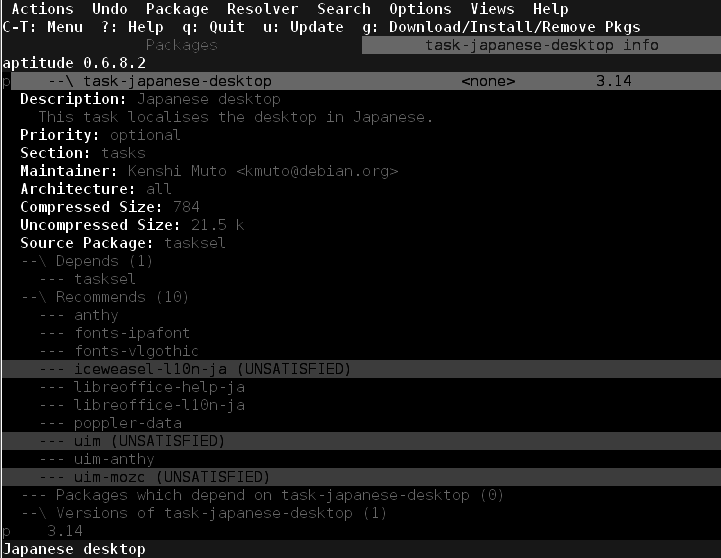
\includegraphics[width=8.5cm]{image201212/im01_mono.png}
  \end{center}
  \caption{Japanese desktop}
  \label{fig:one}
 \end{minipage}
 \begin{minipage}{0.5\hsize}
  \begin{center}
   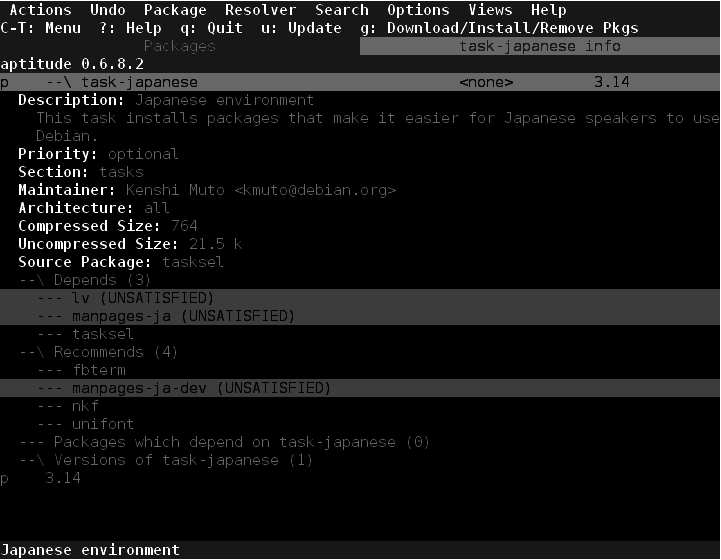
\includegraphics[width=8.5cm]{image201212/im02_mono.png}
  \end{center}
  \caption{Japanese environment}
  \label{fig:two}
 \end{minipage}
\end{figure}

\clearpage
\subsection{日本語入力の選択肢}
DebianのInput method環境(IM環境)とIM Engine(IMエンジン)との組み合わせは下記のように多種あります。
wheezy時点での一般的な日本語入力ユーザへのおすすめは、キーとなるパッケージのibus-anthyやibus-mozcやuim-anthyやuim-mozcといったパッケージから一つを選び、APT系のパッケージ管理プログラム経由で選び導入することです。すると、推薦パッケージも自動的に導入され良好な日本語入力関係が整備されます。
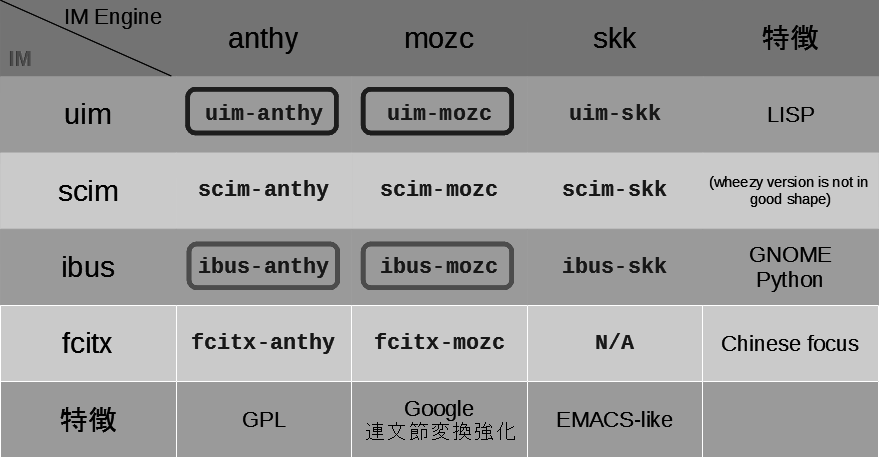
\includegraphics[width=0.7\hsize]{image201212/im03_mono.png}

\subsection{im-configとは}
im-configパッケージはim-switchパッケージの後継のCJKV\footnote{Chinese-Japanese-Korean-Vietnameseの略}入力環境設定支援システムです。
im-configパッケージにより提供されるGUI programのim-configは、複数のIM関連パッケージを導入した際に、システムに導入された数あるIM環境の中の一つを選択し、それらが正しい環境で起動されるように設定します。(IMエンジンの設定は、各IM環境が提供する設定プログラム経由で行います。)
単一IM環境がインストールされる場合には、im-configパッケージによる自動設定で十分です。
im-configパッケージが導入するフックスクリプトは/etc/X11/Xsession.d/70im-config\_launchにあります。
GDMやstartxが /etc/X11/Xsession経由でこのフックスクリプトを呼び、dbusの設定後、下記の様にClient環境変数を設定し、
\begin{commandline}
XMODIFIERS=@im=ibus
GTK_IM_MODULE=ibus
QT4_IM_MODULE=ibus
...等
\end{commandline}
数ある導入されたIM環境の中の一つを選び、それを起動します\footnote{例えば、ibusの場合には「/usr/bin/ibus-daemon --daemonize -xim」が起動されます。}。
\\
実際にIM環境やIMエンジンの設定を有効にするのは、以下のアクションが必要ですので注意して下さい。
\begin{itemize}
\item IM環境設定にはXの再起動が必要です。通常、アカウントからログアウト後の再ログインで実現します。
\item IMエンジン設定にはIM環境の再起動が必要です。通常、トレイ等にあるIMエンジンの設定プログラムアイコンを右クリックして実現します。
\end{itemize}
\clearpage
\subsection{im-configの日本語GUI}
im-configプログラムは日本語化対応されたシェルスクリプトで実装されたメニュープログラムです。通常はGTKのGUIで表示されます。im-configに-cオプションをつけて起動することで、最後のスクリーン例のようにターミナルの下でもメニュー表示ができます。
\begin{figure}[htbp]
 \begin{minipage}{0.5\hsize}
  \begin{center}
   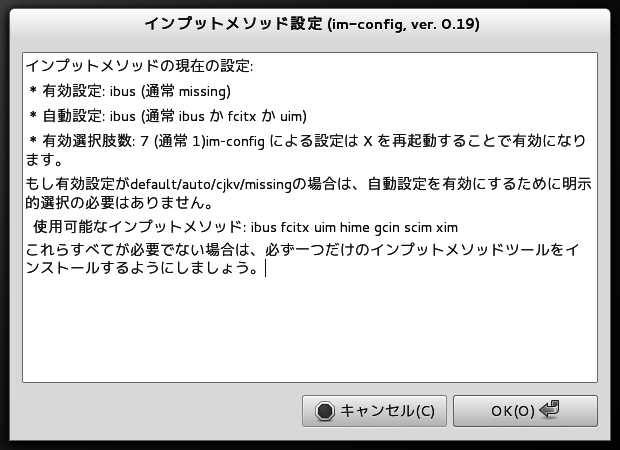
\includegraphics[width=8cm]{image201212/im04_mono.png}
  \end{center}
  \label{fig:one}
 \end{minipage}
 \begin{minipage}{0.5\hsize}
  \begin{center}
   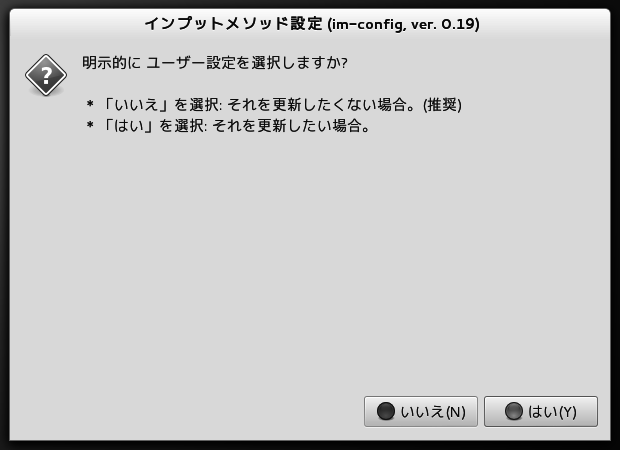
\includegraphics[width=8cm]{image201212/im05_mono.png}
  \end{center}
  \label{fig:two}
 \end{minipage}
\end{figure}

\begin{figure}[htbp]
 \begin{minipage}{0.5\hsize}
  \begin{center}
   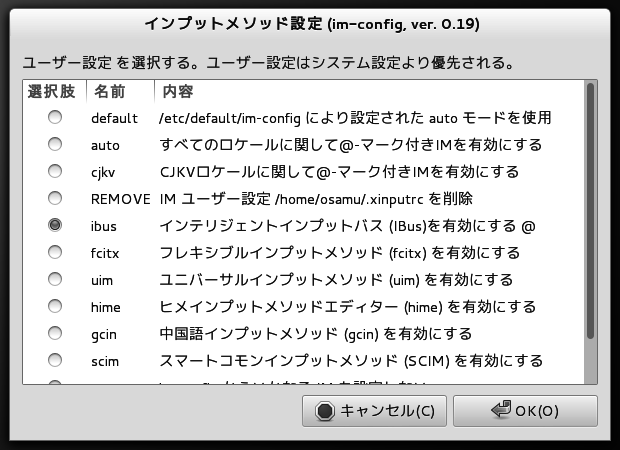
\includegraphics[width=8cm]{image201212/im06_mono.png}
  \end{center}
  \label{fig:one}
 \end{minipage}
 \begin{minipage}{0.5\hsize}
  \begin{center}
   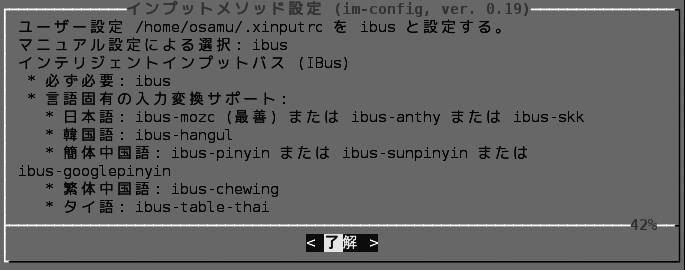
\includegraphics[width=8cm]{image201212/im07_mono.png}
  \end{center}
  \label{fig:two}
 \end{minipage}
\end{figure}

\subsection{/etc/X11/Xsession.d/}
Xの起動時には/etc/X11/Xsession.d/の中にある多くのフックスクリプトが順番に実行されます。この/etc/X11/Xsession.d/の中は大体次のようになっています。
\begin{commandline}
20x11-common_process-args
30x11-common_xresources
35x11-common_xhost-local
40x11-common_xsessionrc
50x11-common_determine-startup
55gnome-session_gnomerc
60xdg-user-dirs-update
70im-config_launch
75dbus_dbus-launch
90apparmor-notify
90consolekit
90gpg-agent
90qt-a11y
90x11-common_ssh-agent
99x11-common_start
\end{commandline}
im-configのフックスクリプトは、これらのフックスクリプトの1つの75dbus\_dbus-launchということは、すぐ分かりますね。
でも、Wheezyのim-configはdbusから起動されるプログラム等にも対応すべく、ちょっと複雑なことをしています。
\\
このフックスクリプト75dbus\_dbus-launchが実行される時(PHASE 1)に、IM関連の環境変数の設定と、\$STARTUPという環境変数の更新設定をしています。
実際この\$STARTUPという環境変数は、他のフックスクリプトででも順次更新設定されます。
\\
そして最後の99x11-common\_startにより、「exec \$STARTUP」が実行される事で\$STARTUPのコマンドが実行されます。
この\$STARTUPが実行される際(PHASE 2)に、/usr/bin/im-launchが呼ばれデーモンのプログラムの起動がされます。

\subsection{im-configのカスタマイズ}
標準設定で動かなければ、X起動時に読み込み実行される~/.xinputrcを使ってカスタマイズしてください。このファイルは、通常im-configをユーザーアカウントから実行することで作成されます。その内容は、基本的にシェルプログラムです。
\\
典型的な~/.xinputrcの例を以下に示します。この内容ですが、im-configパッケージが提供するrun\_imという専用シェル関数によりその引数のibusで指定される/usr/share/im-config/data/ibus.rcを呼びだして、ibusをIM環境として有効とするように設定しています。
\begin{commandline}
# im-config(8) generated on Fri, 14 Dec 2012 00:47:26 +0900
run_im ibus
# im-config signiture: b86f7277b9fc27366da40da0b0553a4a  -
\end{commandline}
この~/.xinputrcの内容を/usr/share/im-config/data/*.rcファイルのコピーで置き換えそれを改変することで、IMに関して更なるカスタマイズができます。(上級者テクニックです。)
その際には以下の2つのルールに注意してシェルプログラムを書いて下さい。
\begin{itemize}
\item "\$IM\_CONFIG\_PHASE" = 1の条件下では、環境変数の設定をします。
\item "\$IM\_CONFIG\_PHASE" = 2の条件下では、デーモンのプログラムの起動をします。
\end{itemize}
もしバグを見つけた際には、バグ報告をreportbugプログラムを使ってim-configパッケージにしてください。

%201304
%-------------------------------------------------------------------------------
\dancersection{debootstrapを有効活用してみよう}{杉本典充}
%-------------------------------------------------------------------------------
\index{debootstrap}

debianのインストール処理に使うdebootstrapコマンドの応用例として開発環境整備、サーバ用途、組み込み用途、異種OS利用とまとめてみました。

\subsection{仮想化技術について}
最近KVMを事例とする「仮想化」という言葉をよく聞くようになりました。仮想化にもいくつかの種類があると思い調べてみたところ、以下の例が見つかりました。今回は、コンテナ型仮想化に着目していきます。

\begin{table}[hb]
  \begin{tabular}{|l|p{10em}|p{20em}|} \hline
    仮想化技術 & 実装例 & 仮想化環境の特徴 \\ \hline
    完全仮想化(エミュレーション型) & QEMU、VirtualBox & 既存のOSを無修正のままゲスト環境として動作させる。ホストOSで動作する仮想化アプリケーションがエミューションする。 \\ \hline
    完全仮想化(ハイパーバイザ型) & KVM & 既存のOSを無修正のままゲスト環境として動作させる。CPU等の仮想化機能を使うことでホスト環境におけるオーバーヘッドを極力減らしている。 \\ \hline
    準仮想化 & Xen & ホスト環境とやりとりするAPIを利用できるように修正が入ったOSをゲストOSとして動作させる方式(=既存のOSそのままでは動かない) \\ \hline
    コンテナ型仮想化 & OpenVZ、LXC、FreeBSD jail & ホスト環境とゲスト環境は同一カーネルで動作しつつ、ホスト環境から分離したゲスト環境を提供する。  \\ \hline
  \end{tabular}
\end{table}

\subsection{debianにおけるコンテナ環境の作り方}

\subsubsection{debootstrap}
debianにおいてコンテナ型仮想化の環境を構築する機能としてdebootstrapがあります。debootstrapを実行すると、debianをインストールしたときのルートディレクトリ構造を任意のパスに作成することができます。

debootstrapのインストールは以下のapt-getコマンドで実行できます。deboostrapにはdebootstrap(shスクリプトで実装)とcdebootstrap(C言語で実装)の2種類のコマンドがあります。

\begin{commandline}
$ sudo apt-get install debootstrap cdebootstrap
$ sudo mkdir -p /srv/chroot
$ cd /srv/chroot
$ sudo debootstrap --arch=amd64 sid ./mysid http://ftp.jp.debian.org/debian
$ ls mysid
bin   dev  home  lib64  mnt  proc  run   selinux  sys  usr
boot  etc  lib   media  opt  root  sbin  srv      tmp  var
\end{commandline}

\subsubsection{chrootコマンド}
\index{chroot}

debootstrapで作成したコンテナ環境でプログラムを実行したいのですが、環境変数とディレクトリの配置が合わないためうまくコマンドを実行することができません。そこでchrootコマンドを使います。\footnote{chrootシステムコールは1982年にビル・ジョイが作成したものが起源とされています。ビル・ジョイはプログラムをクリーンビルドできる環境がほしかったため通常利用の環境と分離する手段として開発したと言われています。} \footnote{クリーンビルド目的でchrootコマンドを使う手法ではdebianパッケージのビルドにも使われています。}

chrootコマンドを実行するとルートディレクトリでない場所をあたかもルートディレクトリであるように見せることができます。これにより普通にdebianをインストールした状態のプログラムの配置とPATH環境変数がうまく合い、コンテナ環境のプログラムを実行できるようになります。

\begin{commandline}
$ sudo chroot /srv/chroot/mysid
# pwd
/
# ls
bin   dev  home  lib64  mnt  proc  run   selinux  sys  usr
boot  etc  lib   media  opt  root  sbin  srv      tmp  var
\end{commandline}

chrootコマンドにも現在ではいくつかの派生版があります。

\begin{itemize}
  \item chroot
  \begin{itemize}
    \item 元祖chroot。実行するにはroot権限が必要。
  \end{itemize}
  \item dchroot
  \begin{itemize}
    \item chrootを一般ユーザで実行できるように改良した版。(とはいえdebootstrapと設定ファイル作成はroot権限が必要)
  \end{itemize}
  \item schroot
  \begin{itemize}
    \item dchrootのセキュリティレベルを向上させた改良版。
  \end{itemize}
\end{itemize}

今度はschrootコマンドでコンテナ環境に入ってみます。
\index{schroot}

\begin{commandline}
$ sudo apt-get install schroot
$ cd /etc/schroot
$ sudo vi schroot.conf

[mysid]
description=my sid for devel
type=directory
directory=/srv/chroot/mysid
users=norimitu
root-groups=root
personality=linux
preserve-environment=true

$ schroot -c mysid
W: Failed to change to directory ‘/etc/schroot’: No such file or directory
I: The directory does not exist inside the chroot.  Use the --directory option to run the command in a different directory.
W: Falling back to directory ‘/home/norimitu
$ ls -la /srv
total 8
drwxr-xr-x  2 root root 4096 Apr 14 02:59 .
drwxr-xr-x 22 root root 4096 Apr 14 03:04 ..

(何もないです。chroot環境に入っています)
$ cd /home/norimitu
$ ls
(chroot元のホスト環境のファイルが出てくる。)
\end{commandline}

直感的にはchrootコマンドの方がわかりやすいです。

schrootコマンドの場合は、schrootした環境内のホームディレクトリはホスト環境のホームディレクトリとbindされます。そのため、ホスト環境にあるファイルをschrootした環境からそのまま読み書きできます。(chrootの場合はそういう仕組みがないため、コピーする必要がある。)

\subsection{debootstrapの使いどころ}

debootstrapを使うと何が便利なのか使いどころの例を上げてみます。

\subsubsection{生活環境と開発(テスト)環境を分離する}

普段使用する環境はstableを利用するが、バージョン等の都合で部分的にsidで提供されているパッケージを利用したい場合があります。その場合、前述した方法でコンテナ環境を作成し、chrootすれば利用できます。

\subsubsection{コンテナ内で異なるCPUアーキテクチャの環境を動かす}

debootstrapしたコンテナ環境は通常ホスト環境で動作するCPUアーキテクチャで構築します。chrootコマンドでコンテナ環境に入っている場合でもカーネルはホストOSと同じため、異なるCPUアーキテクチャのバイナリをネイティブに実行できないためです。

amd64カーネルを実行しているマシンの場合、i386バイナリは実行できますのでi386環境のコンテナ環境を構築すれば実行できます。

私は諸般の都合でamd64環境のVPS上でi386のpostgresql-9.1を動かしてレプリケーションしています。amd64とi386間といったCPUアーキテクチャが異なる場合はレプリケーションができないpostgresqlの仕様になっているため、VPSのホストOSはamd64、コンテナ内でi386環境を動かしてレプリケーションしています。

% personality flags も考えると多分 linux32 コマンド使ったほうが良いと思
% う --dancerj
\begin{commandline}
$ sudo mkdir -p /srv/chroot
$ cd /srv/chroot
$ sudo debootstrap --arch=i386 sid ./mysid-i386 http://ftp.jp.debian.org/debian
$ sudo chroot ./mysid-i386
# uname -a
Linux www6368uj 3.2.0-4-amd64 #1 SMP Debian 3.2.41-2 x86_64 GNU/Linux
# apt-get install file
# file /bin/ls
/bin/ls: ELF 32-bit LSB executable, Intel 80386, version 1 (SYSV),
dynamically linked (uses shared libs), for GNU/Linux 2.6.26,
BuildID[sha1]=0x498625fc854816515ec12819544ebedff51d5c32, stripped
\end{commandline}

また、chrootとQEMUを組み合わせることにより、ホストOSのカーネルでは動作しないCPUアーキテクチャのコンテナ環境をQEMUを使ったエミュレートで動作させることができます。最近流行りの安価なARMボードでdebianを動作させるためのディレクトリツリーを作成するのに便利です。\footnote{実際にARMボード上でdebianを起動させるためにはSDカード等へのファイルシステム作成、カーネルやドライバの作成、ブートローダーの書き込み等、色々やらないと動きません。}

ホスト環境と異なるCPUアーキテクチャのコンテナ環境をchrootする場合、以下の手順で実行する必要があります。

\begin{itemize}
  \item debootstrapは「--foreign」引数を渡して実行すること
  \item コンテナ環境内に「qemu-*-static」ファイルをコピーしておくこと(例:qemu-arm-static)
  \item chrootで入った後でdebootstrapのsecond stageを実行すること
\end{itemize}

\index{arm}
\index{qemu}
\index{qemu-user-static}
\index{qemu-arm-static}
\begin{commandline}
$ sudo apt-get install binfmt-support qemu qemu-user-static debootstrap
$ sudo mkdir -p /srv/chroot
$ cd /srv/chroot
$ sudo debootstrap --foreign --arch=armel wheezy ./armdev1 http://ftp.jp.debian.org/debian
$ sudo chroot ./armdev1
chroot: コマンド `/bin/bash' の実行に失敗しました: No such file or directory

$ sudo cp /usr/bin/qemu-arm-static /srv/chroot/armdev1/usr/bin/
$ sudo chroot armdev1
I have no name!@hostname:/#
Linux hostname 3.2.0-4-amd64 #1 SMP Debian 3.2.41-2 armv7l GNU/Linux

I have no name!@hostname:/# apt-get update
bash: apt-get: command not found
I have no name!@hostname:/# ls /debootstrap
arch  debootstrap      debpaths        functions  suite
base  debootstrap.log  devices.tar.gz  required   suite-script
I have no name!@hostname:/# /debootstrap/debootstrap --second-stage
I: Installing core packages...
I have no name!@hostname:/# apt-get update
Reading package lists...

I have no name!@hostname:/# vi /etc/apt/sources.list

deb http://ftp.jp.debian.org/debian wheezy main
deb-src http://ftp.jp.debian.org/debian wheezy main

deb http://security.debian.org/ wheezy/updates main
deb-src http://security.debian.org/ wheezy/updates main

I have no name!@hostname:/# apt-get update
I have no name!@hostname:/# apt-get install file
I have no name!@hostname:/# file /bin/ls
/bin/ls: ELF 32-bit LSB executable, ARM, version 1 (SYSV),
dynamically linked (uses shared libs), for GNU/Linux 2.6.26,
BuildID[sha1]=0x5bc97dbca9ac168932d898a5e2eaf68e8fde5e16, stripped
\end{commandline}


\subsubsection{サーバでたくさんのコンテナを常駐させて動かしたい}

今までのコンテナ環境は手でコマンドを実行することでコンテナ環境に入っていました。コンテナ環境をサーバのように動かしたいというニーズもあります。今回はDebian GNU/Linux wheezy amd64上でLXC(Linux Containers)を用いてコンテナ環境を常駐させてみます。

まずホスト環境の設定と環境を確認します。

\begin{commandline}
$ sudo apt-get install lxc
$ sudo vi /etc/fstab

(追記します)
cgroup  /sys/fs/cgroup  cgroup  defaults  0   0

$ sudo mount -a
$ lxc-checkconfig
Kernel config /proc/config.gz not found, looking in other places...
Found kernel config file /boot/config-3.2.0-4-amd64
--- Namespaces ---
Namespaces: enabled
Utsname namespace: enabled
Ipc namespace: enabled
Pid namespace: enabled
User namespace: enabled
Network namespace: enabled
Multiple /dev/pts instances: enabled

--- Control groups ---
Cgroup: enabled
Cgroup clone_children flag: enabled
Cgroup device: enabled
Cgroup sched: enabled
Cgroup cpu account: enabled
Cgroup memory controller: enabled
Cgroup cpuset: enabled

--- Misc ---
Veth pair device: enabled
Macvlan: enabled
Vlan: enabled
File capabilities: enabled

Note : Before booting a new kernel, you can check its configuration
usage : CONFIG=/path/to/config /usr/bin/lxc-checkconfig
\end{commandline}

LXCで動作するコンテナ環境のネットワークはホスト環境とブリッジ接続する必
要があります。
\index{lxc}

ここではeth0はそのままでブリッジデバイスを1つ作成し、LXCのコンテナ環境はブリッジデバイスのNAT環境下で動作することとします。\footnote{http://wiki.debian.org/LXC/SimpleBridge}

\begin{commandline}
$ sudo vi /etc/sysctl.conf

(変更)
net.ipv4.ip_forward=1

$ sudo sysctl -p
net.ipv4.ip_forward = 1

$ vi br-lxc.sh
# script to setup a natted network for lxc guests
CMD_BRCTL=/sbin/brctl
CMD_IFCONFIG=/sbin/ifconfig
CMD_IPTABLES=/sbin/iptables
CMD_ROUTE=/sbin/route
NETWORK_BRIDGE_DEVICE_NAT=lxc-bridge-nat
HOST_NETDEVICE=eth0
PRIVATE_GW_NAT=192.168.20.1
PRIVATE_NETMASK=255.255.255.0
PRIVATE_NETWORK=192.168.20.0/24

${CMD_BRCTL} addbr ${NETWORK_BRIDGE_DEVICE_NAT}
${CMD_BRCTL} setfd ${NETWORK_BRIDGE_DEVICE_NAT} 0

${CMD_IFCONFIG} ${NETWORK_BRIDGE_DEVICE_NAT} ${PRIVATE_GW_NAT} netmask ${PRIVATE_NETMASK} promisc up

${CMD_IPTABLES} -t nat -A POSTROUTING -o ${HOST_NETDEVICE}  -j MASQUERADE
${CMD_IPTABLES} -A FORWARD -i ${NETWORK_BRIDGE_DEVICE_NAT} -o ${HOST_NETDEVICE} -s ${PRIVATE_NETWORK} -j ACCEPT

$ sudo ./br-lxc.sh
$ sudo ifconfig lxc-bridge-nat
lxc-bridge-nat Link encap:イーサネット  ハードウェアアドレス fe:24:c3:eb:6d:c3
          inetアドレス:192.168.20.1 ブロードキャスト:192.168.20.255  マスク:255.255.255.0
          inet6アドレス: fe80::409a:3cff:fee6:33b0/64 範囲:リンク
          UP BROADCAST RUNNING PROMISC MULTICAST  MTU:1500  メトリック:1
          RXパケット:6556 エラー:0 損失:0 オーバラン:0 フレーム:0
          TXパケット:1121 エラー:0 損失:0 オーバラン:0 キャリア:0
      衝突(Collisions):0 TXキュー長:0
          RXバイト:543131 (530.4 KiB)  TXバイト:95778 (93.5 KiB)
\end{commandline}

コンテナを作成します。LXCにおけるコンテナは ``\texttt{/var/lib/lxc}''ディレクトリの下にできます。

\begin{commandline}
$ sudo lxc-create -n lxc-deb1 -t debian
 (ダイアログ形式でインストールするバージョンやダウンロード先ミラーのURL、
  rootパスワードが聞かれるので答える) 

$ cd /var/lib/lxc/lxc-deb1
$ ls
config    rootfs
$ sudo vi config

(追記します)
## Network
lxc.utsname = lxc-deb1
lxc.network.type = veth
lxc.network.flags = up

# that's the interface defined above in host's interfaces file
lxc.network.link = lxc-bridge-nat

# name of network device inside the container,
# defaults to eth0, you could choose a name freely
# lxc.network.name = lxcnet0

lxc.network.hwaddr = 00:FF:AA:00:00:01

# the ip may be set to 0.0.0.0/24 or skip this line
# if you like to use a dhcp client inside the container
lxc.network.ipv4 = 192.168.20.101/24
\end{commandline}

LXCコンテナ内でsshdが起動するよう設定しておきます。

\begin{commandline}
$ sudo cp /etc/resolv.conf /var/lib/lxc/lxc-deb1/rootfs/etc/
$ sudo vi /var/lib/lxc/lxc-deb1/rootfs/etc/ssh/sshd_config

(変更前)  #ListenAddress 0.0.0.0
(変更後)  ListenAddress 192.168.20.101 
\end{commandline}

LXCコンテナを起動します。``-d''オプションはバックグラウンドで起動させるオプションです。これでコンテナ環境が常駐して動作するようになります。

\begin{commandline}
$ sudo lxc-start -n lxc-deb1
Using makefile-style concurrent boot in runlevel 2.
Starting OpenBSD Secure Shell server: sshdCould not load host key: /etc/ssh/ssh_host_rsa_key
Could not load host key: /etc/ssh/ssh_host_dsa_key

なぜかssh鍵を作る処理が自動実行されず止まってしまうため、手動で作ってみる。
$ sudo chroot /var/lib/lxc/lxc-deb1/rootfs ssh-keygen -t dsa -f /etc/ssh/ssh_host_dsa_key
$ sudo chroot /var/lib/lxc/lxc-deb1/rootfs ssh-keygen -t rsa -f /etc/ssh/ssh_host_rsa_key

$ sudo lxc-start -n lxc-deb1 -d
$ ssh root@192.168.20.101
root@lxc-deb1:~#

 ログインできました。

$ sudo lxc-stop -n lxc-deb1
\end{commandline}

\subsubsection{異なるOS上でdebianを構築する}

\index{kfreebsd-amd64}
\index{freebsd}
\index{jail}
debootstrapは異なるOS上でdebianを構築することができます。ここでは、FreeBSD-8.3-RELEASE amd64のjail機能を用いてkfreebsd-amd64をprisonerとして動かしてみます。\footnote{http://blog.vx.sk/archives/22-Updated-Tutorial-Debian-GNUkFreeBSD-in-a-FreeBSD-jail.html}

まずはjail環境を作成するためのツールをインストールします。

OSが異なるとdebootstrapコマンドがないため、tarball(中身はshスクリプト版)をダウンロードして実行します。\footnote{portsで/usr/ports/sysutils/debootstrapもありますのでそちらを使ってもいいです}

\begin{commandline}
> cd
> wget http://ftp.jp.debian.org/debian/pool/main/d/debootstrap/debootstrap_1.0.48.tar.gz
> tar xf debootstrap_1.0.48.tar.gz
> cd debootstrap-1.0.48
# su
# setenv DEBOOTSTRAP_DIR `pwd`
# ./debootstrap --arch=kfreebsd-amd64 wheezy /usr/jails/jailkfdeb http://ftp.jp.debian.org/debian
# kldload fdescfs linprocfs linsysfs tmpfs
# umount /usr/jails/jailkfdeb/dev/fd
# umount /usr/jails/jailkfdeb/dev
# mount -t linprocfs linprocfs /usr/jails/jailkfdeb/proc
# mount -t linsysfs linsysfs /usr/jails/jailkfdeb/sys
# mkdir -p /usr/jails/jailkfdeb/lib/init/rw
# mount -t tmpfs tmpfs /usr/jails/jailkfdeb/lib/init/rw
# cp /etc/resolv.conf /usr/jails/jailkfdeb/etc/resolv.conf
\end{commandline}

\begin{commandline}
> sudo portsnap fetch
> sudo portsnap update
> cd /usr/ports/sysutils/ezjail
> sudo make
> sudo make install

> sudo touch /etc/fstab.jailkfdeb
  (このファイルがないとエラーになるためとりあえず作成します)
> vi /etc/rc.conf
(追記します)
ifconfig_em0_alias0="inet 192.168.1.63/32"

> ifconfig em0 192.168.1.63 netmask 255.255.255.255 alias
> vi /usr/local/etc/ezjail/jailkfdeb

# To specify the start up order of your ezjails, use these lines to
# create a Jail dependency tree. See rcorder(8) for more details.
#
# PROVIDE: standard_ezjail
# REQUIRE:
# BEFORE:
#

export jail_jailkfdeb_hostname="jailkfdeb"
export jail_jailkfdeb_ip="192.168.1.63"
export jail_jailkfdeb_rootdir="/usr/jails/jailkfdeb"
export jail_jailkfdeb_exec_start="/etc/init.d/rc 3"
export jail_jailkfdeb_exec_stop=""
export jail_jailkfdeb_flags="-l -u root"
export jail_jailkfdeb_mount_enable="YES"
export jail_jailkfdeb_devfs_enable="YES"
export jail_jailkfdeb_devfs_ruleset="devfsrules_jail"
export jail_jailkfdeb_procfs_enable="YES"
export jail_jailkfdeb_fdescfs_enable="YES"


> sudo /usr/local/etc/rc.d/ezjail start jailkfdeb
Configuring jails:.
Starting jails: jailkfdeb.
> jls
   JID  IP Address      Hostname                      Path
    11  192.168.1.63    jailkfdeb                     /usr/jails/jailkfdeb
> su
# jexec 11 /bin/sh

(ここからコンテナ環境の中です)

# uname -irps
GNU/kFreeBSD 8.3-RELEASE-p6 amd64 Intel(R) Core(TM) i5-2500S CPU @ 2.70GHz
# vi /etc/apt/sources.list

deb http://ftp.jp.debian.org/debian wheezy main contrib non-free
deb-src http://ftp.jp.debian.org/debian wheezy main contrib non-free

# apt-get update
# apt-get install openssh-server
# vi /etc/ssh/sshd_config

修正前)  #ListenAddress 0.0.0.0
修正後)  ListenAddress 192.168.1.63

# /etc/init.d/ssh restart
# passwd
# exit

(コンテナ環境からホスト環境に戻ります)

> ssh root@192.168.1.63 
\end{commandline}

sshでコンテナ環境にログインできました。

\subsection{参考情報}

\begin{itemize}
  \item{Debian Wiki Schroot http://wiki.debian.org/Schroot}
  \item{Debian Wiki LXC http://wiki.debian.org/LXC}
  \item{Debian Wiki EmDebianCrossDebootstrap http://wiki.debian.org/EmDebian/CrossDebootstrap}
  \item{関西エリアDebian勉強会 2009年04月号「Debian を新規に install してから常用環境にするまで」 佐々木洋平}
  \item{Updated Tutorial: Debian GNU/kFreeBSD in a FreeBSD jail  http://blog.vx.sk/archives/22-Updated-Tutorial-Debian-GNUkFreeBSD-in-a-FreeBSD-jail.html}
\end{itemize}

%201301kansai
\dancersection{Using Drupal on Debian − CMSから入った人のDebian体験}{紀野 惠}
\index{drupal}

\subsection{はじめに}

今回はDrupalの紹介と共に、Linux初心者のWeb製作者がどのようにDebianを触ってきたかをお話しするつもりです。

サーバーホスティングがどんどん低価格化し、CMS・WebアプリをVPSや専用サーバー、あるいはAMAZON EC2のようなクラウド環境で動かすことへの敷居も下がってきています。

特にVPSに関して日本は現状世界で一番競争が激しくコストパフォーマンスの高い環境が手に入ります。
これまで共用サーバーでを動かしていたときには手が届かなかったライブラリの導入やパフォーマンス・チューニングが出来るようになり、自由度も性能も一度に手に入れることができるのですが、一方でOSとPHP,MySQLなどのミドルウェアをまるごと自分でメンテナンスしなければならなくなりました。

今後もますます増えていくであろうDrupalやWordpressなどのCMSユーザーにDebianを使ってもらい、コミュニティがさらに活性化する参考にしてもらえばうれしく思います。

\subsubsection{自己紹介}
\begin{itemize}
\item[名前] 紀野 惠(きの さとし)

  Twitter: @qchan\_kino

  Facebook: satoshi.kino

\item[所属] ANNAI LLC \url{http://an-nai.jp}

  ジオどす \url{http://geodosu.com}

  などあれこれ。
\end{itemize}

\url{http://groups.drupal.org/japan/} で活動しています。

OSC京都、KOF実行委員やOSS勉強会運営のお手伝いなども。KOF2012はDrupalで動いてます!

\clearpage

\subsection{Drupalって?}
CMSでもあり、Webアプリケーションフレームワークでもあります。

\subsubsection{要件}
\begin{itemize}
\item License: GPL 2
\item Web Server: Apache, Nginx, or Microsoft IIS
\item PHP: 5.3以上推奨  PDO必須
\item DB: MySQL, PostgreSQL, SQLite
  (MS SQL Server, Oracle はモジュールで対応)

\cite{requirements}
\end{itemize}

開発環境では Sqliteがオススメ(さっと立ち上がってポータビリティに優れています)。

\subsubsection{人気}

\begin{itemize}
\item Open Source Awards 優勝多数でアワード殿堂入り
\item インストールベースのシェア3位(1位はWordpress,2位はJoomla!)
\end{itemize}

\subsubsection{採用実績}
世界中の有名サイトでの採用実績多数
\begin{itemize}
\item Whitehouse
\item Harvard University
\item Econmist
\item 毎日jp
\item Computer World
\item Ubuntu
\item Linux Foundation
\item SONY MUSIC ENTERTAINMENT
\end{itemize}

など多すぎて書ききれません。

ブログ的な情報発信型だけでなく、会員コミュニティサイトのように内部で動きのあるサイトを得意としています。

大学、政府系では海外で非常に強い信頼を得ています。

\subsubsection{特徴}
一企業発のプロダクトではなく、完全にコミュニティーベースのOSS。

\begin{itemize}
\item 拡張性の高いアーキテクチャ
\item 豊富なAPIとHockシステム
\item オーバーライドの仕組み
\item 専門のセキュリティチームがおり、脆弱性が報告されれば迅速に対応
\end{itemize}

今時のCMSはどれもカスタマイズの機構を備えていますが、Drupalはその拡張性が非常に高く、オーバーライドできることを重要視して作られていますので、ダーティーなハックを極力減らせます。

\subsubsection{開発状況}
Webの流れを常にキャッチアップしていこうとしています。次期バージョンDrupal8は真にフレームワーク化しそう。

Restful、Symfony2採用など大きく変わります。

\subsubsection{得意分野}
大規模サイトの構築を得意としています。
\begin{itemize}
\item リバースプロキシ
\item DBレプリケーション標準対応
\item Memcacheや静的ファイルキャッシュも可能
\item Varnish, nginx ,APCなどでのキャッシュ対応が容易
\end{itemize}

\subsubsection{多言語対応・共同翻訳システム}
標準で多言語対応。
また、\url{http://localize.drupal.org} でコア + 全モジュールの共同翻訳システムが稼働。

\subsubsection{マルチドメイン、マルチサイト}
標準で対応しています。

\subsubsection{コミュニティ}
世界中の活発なコミュニティで開発されています。

毎年、春はアメリカ、秋はヨーロッパで大規模なカンファレンスも開催

\begin{itembox}[l]{Drupalcon Munich}
  \begin{itemize}
  \item 日時:2012 年 8 月 20 日 〜 24 日
  \item 参加人数:1800人
  \item 収入 Total Revenue \euro 892,221(約9100万円)/支出 Total Expenses \euro 858,366(約8700万円)
  \end{itemize}
\end{itembox}

\subsubsection{豊富なモジュール}
\begin{itemize}
\item 提供されているモジュールの数は 5,000以上
\item 全モジュールをコミュニティ内でGit管理。
\item drupal.org内にIssueやPatch等、全てが集約されている。
\end{itemize}

たくさんのモジュールがあることで有名なDrupalだが、、、モジュールの組み合わせ、実装方法が何通りも存在します。

柔軟性が高い反面、学習カーブが厳しいと言われることがあります。

そうした声を反映してか、最近はインストールしてそのまま使えるディストリビューションがとても増えてきました。

\subsubsection{ディストリビューション}

\begin{itemize}
\item アメリカ政府のホワイトハウスが配布しているディストリビューション。市民からの請願・情報を集約するサイト。
\item ハーバード大学が開発・配布している教育機関向けディストリビューション
\item Eコマース向けディストリビューション
\item Open Data特化型ディストリビューション
\item CRMのディストリビューション
\item PostGIS、GeoServer、OpenLayersのセットになっているGeoMediaに特化したディストリビューション
\item カンファレンス参加登録、セッション登録、スケジューリング、チケット決済まで可能な大規模なカンファレンス用サイトを作成できるディストリビューション
\end{itemize}

など様々公開されています。
\cite{distributions}


\subsection{LinuxディストリビューションでDebianを選んだ理由}
\begin{itemize}
\item 超安定
\item Drupalを使うための情報が圧倒的に多い。(Ubuntu含む)
\item 検索のために単語登録してます $-$ "で" $=$ (debian $|$ ubuntu) drupal
\item パッケージが多い
\item メジャーバージョンアップが可能
\item 個々のパッケージのバージョン固定ができる
\end{itemize}

\begin{itembox}[l]{一番重要なポイント}
 コミュニティが活発。勉強会で直接話を聞ける。
\end{itembox}


\subsection{DebianでDrupalなどのCMS・Webフレームワークを使うには・・・}
\subsubsection{DebianのPHPバージョンを変えたいときの対処法}
\begin{itemize}
\item 下げるのは以前のバージョンなどから比較的容易に持ってこれるが、上げるのは依存問題を解決できないことが多い
  しかし極力、ソースからのコンパイルは避けたい。
\item Dotdebにお世話になってます。\cite{dotdeb}

  リリースの端境期などDebianパッケージがセキュリテイパッチを当ててくれないときにも便利

  {\bf OSアップグレード時には外す事}
\end{itemize}

\subsubsection{マニュアルインストールの場合}

\begin{enumerate}
\item ソース

PHPのWebアプリはだいたいファイル一括配置。

Drupal、Wordpress、Typo3、OpenPNEなどほとんど同じ。
\begin{enumerate}
\item {\tt /var/www/}以下にtarボール解凍
\item DBを作成
\item ApacheのVhost設定
\item ブラウザからインストーラーにアクセス
\end{enumerate}

\item Drush

Drupalで共用サーバーを卒業したならまず何を置いても使えるようにしたい。
\begin{itemize}
\item Drush - drupal shell\cite{drush}
\item ブラウザからだと煩雑なDrupalの操作をシェルから操作できるようになる。
\item PEARからのインストールがおすすめ。Drushは開発スピードが早いので頻繁なアップデート追従が楽。
\item 事前課題VMはファイル直置きなのでdrushコマンドそのものを使う。

\begin{commandline}
drush dl drush --destination=/usr/local/share/
\end{commandline}

\clearpage

\item Drushに出来る事
  \begin{itemize}
  \item Drupalコア、モジュールのインストール・アンインストール
  \item 簡易WebServer立ちあげ(PHP5.4以降はライブラリ不要)
  \item Drupalデプロイ
  \item Drupalコア、モジュールのアップデート
  \item Drupalのサイトファイルとデータベースのスナップショット作成
  \item スナップショットからのリストア
  \item キャッシュクリア
  \item 複数サイトの一括コマンド操作
  \item DB操作全般
  \item Drupal設定変数操作
  \item Drupal状況の表示
  \item モジュールのPatchをURLから当てる
  \item ユーザー追加
  \item パスワード変更
  \item ロール変更・追加
  \item make fileからのDrupalディストリビューションインストール
  \end{itemize}

  モジュールとの連携でまだまだ出来る事が増え続けている。
\end{itemize}
\end{enumerate}

\subsection{パッケージインストールの場合}

\begin{itemize}
\item {\tt apt-get install drupal7}だけ。

非常に簡単。素晴らしい。
\item ただし、マニュアルインストールとは互換性がないので混ぜないように。\cite{ubuntudoc}
\item ここで問題。どこがどう変化したのかわからない。
\item まず最初にすべきは{\tt /usr/share/doc/\{パッケージ名\}}の中を読むこと。
\item 設定ファイルはどこか?
  \begin{itemize}
  \item {\tt dpkg --status \{パッケージ名\}}
    \begin{itemize}
      {\tt /etc/cron.d/drupal7}

      {\tt /etc/drupal/7/htaccess}

      {\tt /etc/drupal/7/sites/default/settings.php}

      {\tt /etc/drupal/7/apache2.conf}
    \end{itemize}
  \end{itemize}
\item パッケージのインストール後の配置を確認するには。
  \begin{itemize}
  \item Debianパッケージページのlist of files\cite{filelist}
  \item {\tt dpkg -L \{パッケージ名\}}
  \item {\tt apt-file list \{パッケージ名\}}\footnote{インストールされてなくてもOK}
  \item {\tt locate \{パッケージ名\}} \footnote{本来の使い方ではない}

\clearpage

  \item ざっくりファイル配置の変化 (*)はパッケージメンテナが追加したファイル
    \begin{itemize}
    \item {\tt /usr/share/drupal7}

      ほとんどのDrupal関係ファイルはここ。残りはこのディレクトリへのシンボリックリンクとなっている。実質のDrupalルートディレクトリ

    \item {\tt /var/lib/drupal7/files}

      {\tt /var/lib/drupal7/backups} (*)

      アップロードされたファイル・ディレクトリ

    \item {\tt /etc/drupal/7}

      {\tt .htaccess}、 {\tt /sites}以下 {\tt /profile} 以下などユーザーが変更する設定やファイル類を配置

    \item {\tt /var/www}

      Drupalルートディレクトリ({\tt /usr/share/drupal7})へのシンボリックリンク

    \item {\tt /etc/cron.d/drupal7} (*)

      パッケージが用意しているcronファイル

    \item {\tt /etc/drupal7/apache2.conf} (*)

      Apache2の設定ファイル {\tt /etc/apach2/conf.d} へシンボリックリンクを貼って使う

    \item {\tt /var/lib/drupal7/backups} (*)

      パッケージが用意しているバックアップスクリプト用と思われる

    \item {\tt /usr/share/doc/drupal7/scripts/} 以下 (*)

      パッケージが用意しているさまざまなシェルスクリプト群

    \item {\tt /etc/dbconfig-common/drupal7.conf} (*)

      パッケージが生成するコンフィグファイル

    \item {\tt /usr/share/doc/drupal7/dbconfig.template} (*)

      パッケージが用意しているデータベースコンフィグサンプル
    \end{itemize}

  \item 最初、どのような考えでこうなっているのかに戸惑った。
    \begin{itemize}
    \item {\tt FHS(Filesystem Hierarchy Standard)} に従っている。\cite{policyfhs}\cite{wikifhs}
    \item 設定ファイルは {\tt /etc}以下に置かなければならない。\cite{policyfiles}
    \item SELinuxの問題も。
      {\tt /var/lib/drupal7/files}などは、SELinuxの絡みでこうなったらしい。Redhat系も同じ。\cite{bugselinux}
    \end{itemize}

  \item 番外
    \begin{itemize}
    \item Redhat系のdrupalリポジトリも似たようなパッケージファイル配置でした。DBやApacheの設定ファイルを作成するスクリプトなどは独自
    \item Wordpressはどうなってる?
      \begin{itemize}
      \item Wordpressの最新版はunstableにしかないが、パッケージ配置構成は大幅に変わっている。今からならunstableを入れておいたほうが良いだろう。
      \item 独自の設定スクリプトを作って、Webからアクセス。
      \item wp-content以下を {\tt /var/lib} と {\tt /usr/share/wordpress} に分割している。SELinux対策かも。
      \item Flashを使ったツールが同梱されているので、パッケージには含めていないので別途インストールしなさいと書いてある。
      \item {\tt /var/www/}以下にドキュメントルートのシンボリックリンクを置かず、Apache2から{\tt /usr/share/wordpress}に直接振り分けろと書いてある。
      \item 独自のapache.confサンプル
      \item MySQLのセットアップはスクリプトを作ってくれている。
      \item それぞれパッケージメンテナーの考え方が違うのがわかって面白い。
      \end{itemize}
    \end{itemize}
  \end{itemize}
\end{itemize}

\subsection{Drupalに限った場合のDebian package のデメリット}
\begin{itemize}
\item UpstreamのDrupalと何が変わったのかがわかりにくい。
\item バージョンが古い。5000以上もあるモジュールのパッケージ化は難しい。
\item Drushが使えない。
\item ローカルや他のディストリなど別環境へ移行がしにくい。
  \footnote{本来サーバー移行時に必要なファイルは{\tt /sites}以下とDBdumpだけだが、ファイルが分割されてしまうのでDrushでの自動デプロイ、Drupalホスティング管理ツールAegirなどからの操作ができない。\cite{aegir}}


\item Drupalコミュニティで共有されている情報との食い違いが多く戸惑う。初心者ならなおさら難しい。
\end{itemize}


\subsection{Debian 初心者が悩んだポイントと素朴な疑問}
\begin{enumerate}
\item {\tt /usr/share/doc/\{パッケージ名\}} にドキュメントがあると知らず右往左往。

  いつもの解凍したtarボール内にREADME.txtなどが入っている感覚に引っ張られる。

\item confファイルの独特な部分に関して日本語情報がもっと欲しい。日本語情報を探すとどうしてもCentOSが多い。
  \begin{itemize}
  \item Apache2
  \item MySQL
  \item iptables

    など
  \end{itemize}

\item パッケージの構成として、Upstreamのディレクトリ構成をそのまま残して、FHSの要請はシンボリックリンクで済ますことって出来ないのでしょうか。

せっかくのDebianパッケージをできるなら使いたい。

\item Stable, Old Stableの2世代までセキュリティアップデートしてもらえたらいいのにと切に希望。
  \begin{itemize}
  \item サーバーを立てるタイミングによっては1年後にメジャーアップグレードが必須のことも。
  \item Ubuntu LTSを選ぶことになるが、Debianとの微妙な違いにまた戸惑ったり。 dist-upgradeってやっちゃっていいの?とか個々の設定も微妙に違う。
  \item ほんとに実用的かどうかは別にしてRedHatクローンのサポート10年はちょっとうらやましかったりする。
  \end{itemize}

\item 動いているサーバーのメジャーバージョンアップはやっぱりドキドキする。できるならばしたくない。
  \begin{itemize}
  \item 皆さん、どうしてますか?
  \item リリース時にハンズオンを企画して欲しい!
  \item アップグレードをテストする同一環境を作るにはどういう方法がありますか?
  \item アップグレードスクリプトのconfファイルを置き換えますか? にどう対応してよいかわからない。ベストプラクティスってありますか?
  \item Grubで躓いて再起動できなくなった事あり。コンソールがないVPSなどだとジエンド。
  \end{itemize}

\item Stableのローリングリリースってできないもんでしょうか。

\item パッケージ製作時の意図をDebianパッケージのWebページで読めたらいいのに。

なぜ、このような組み換えをしたのかを説明があると理解しやすい。confファイルの位置。ドキュメントの場所など。

\item {\tt /etc/apt/preferences} に書くパッケージのPINナンバーの理解が難しい。ここもハンズオン希望。

\item Drupalも同じですが、初心者にしか意味がなくても導入時に書籍があると安心感ありますね。
\end{enumerate}

\subsection{まとめ}
\begin{itemize}
\item Webサイト立ち上げるならDrupalいいですよ。
\item Debianに限らずOSSの開発者、翻訳者の方には普段から大変お世話になっています。

勉強会・Meetupの定期的な主催がどれほど大変かということも多少ながら理解しているつもりですので、68回開催は心底尊敬に値します。

Debian勉強会とコミュニティの方々にお礼を申し上げると共に、今後も初心者ユーザーを導いていただけるようお願いいたします。
\end{itemize}

\begin{thebibliography}{9}

\bibitem{requirements}
System requirements $|$ drupal, \url{http://drupal.org/requirements}

\bibitem{distributions}
Distributions $|$ drupal.org, \url{http://drupal.org/documentation/build/distributions}

\bibitem{dotdeb}
Dotdeb - The repository for Debian-based LAMP servers, \url{http://www.dotdeb.org/}

\bibitem{drush}
Drush $|$ drupal.org, \url{http://drupal.org/project/drush}

\bibitem{ubuntudoc}
Drupal - Community Ubuntu Documentation, \url{https://help.ubuntu.com/community/Drupal}

\bibitem{filelist}
Debian - Filelist of package drupal7/wheezy/all, \url{http://packages.debian.org/wheezy/all/drupal7/filelist}

\bibitem{policyfhs}
Debian JP Project - Debian ポリシーマニュアル - オペレーティングシステム, \url{http://www.debian.or.jp/community/devel/debian-policy-ja/policy.ja.html/ch-opersys.html\#s9.1}

\bibitem{wikifhs}
Filesystem Hierarchy Standard - Wikipedia, \url{http://ja.wikipedia.org/wiki/Filesystem_Hierarchy_Standard}

\bibitem{policyfiles}
Debian JP Project - Debian ポリシーマニュアル - ファイル, \url{http://www.debian.or.jp/community/devel/debian-policy-ja/policy.ja.html/ch-files.html\#10.7.2}

\bibitem{bugselinux}
Bug 472642 - SELinux denies access to /etc/drupal/default/files/, \url{https://bugzilla.redhat.com/show_bug.cgi?id=472642}

\bibitem{aegir}
Aegir, \url{http://www.aegirproject.org/}

\end{thebibliography}

%201303tokyo
%-------------------------------------------------------------------------------
\dancersection{ldapvi \& python-ldap で stress-free life}{まえだこうへい}
%-------------------------------------------------------------------------------
\subsection{ストレス溜まってませんか?}

今回の記事はOpenLDAPの管理を行っている人がターゲットです。LDAPサーバを管理している人は多くはないと思いますが、この記事がLDAPの運用で苦労している人の一助になれば良いと思います。LDAPなにそれ?な人もLDAPアカウントやアドレス帳などで知らぬ間に恩恵を受けているということは大いにあるので、明日は我が身と思ってお読み下さい。
また、自分で作ったツールのアカウント管理をLDAPで行いたい、という場合にも参考になると思います。

なお、LDAPの基本的なお話や、DebianシステムでのOpenLDAPの入門については、第61回 関西Debian勉強会(2012年7月)に佐々木さんが発表&資料を掲載されているのでそちらを参照下さい。\footnote{あんどきゅめんてっどDebian2012年冬号8.「Debianで作るLDAPサーバ」 \url{http://tokyodebian.alioth.debian.org/pdf/debianmeetingresume2012-fuyu.pdf}}

\index{LDIF(5)}
\index{RFC2849}
\subsection{stress = LDIF}

LDAPの運用で何が面倒かというと、LDIF(LDAP Data Interchange Format)の作成やパースです。LDAPのデータを作成・更新・削除するには通常、LDIFを作成し、ldapadd/ldapmodify/ldapdeleteコマンドで実行します。一つのオブジェクトはdn(distiguised name, 識別名)から始まり、それにattributeが続きます。複数オブジェクトを記述するには空行で分割します。下記は RFC2849 の ``Example 1: An simple LDAP file with two entries'' からの引用です。\footnote{\url{http://www.ietf.org/rfc/rfc2849.txt}}

\begin{commandline}
version: 1
dn: cn=Barbara Jensen, ou=Product Development, dc=airius, dc=com
objectclass: top
objectclass: person
objectclass: organizationalPerson
cn: Barbara Jensen
cn: Barbara J Jensen
cn: Babs Jensen
sn: Jensen
uid: bjensen
telephonenumber: +1 408 555 1212

dn: cn=Bjorn Jensen, ou=Accounting, dc=airius, dc=com
objectclass: top
objectclass: person
objectclass: organizationalPerson
cn: Bjorn Jensen
sn: Jensen
telephonenumber: +1 408 555 1212
\end{commandline}

データフォーマット自体はさほど難しくありませんが、このデータを一から自分でスクラッチで作成するのはとても面倒だと思いませんか?例えば上記のようなユーザアカウントの場合、人間にとってはTSVなどの形式を表計算ソフトで読んだり編集したりすることでしょう。そこからLDIFに変換したり、あるいはその逆はどうしますか?簡単に思いつくのは次の二つでしょう。

\begin{enumerate}
  \item 手でちまちま変換する
  \item なんらかのプログラムで一括変換する
\end{enumerate}

前者は転記ミスなどの可能性から論外ですが、管理対象のアカウントが少数ならいっそ割り切ってLDIFを手で作成するのもありでしょう。
しかしユーザ数が大量になるとプログラムで変換しないと時間の無駄です。

\index{slapd-config(5)}
\index{OpenLDAP}
\subsubsection{そして slapd-config}
OpenLDAP 2.3からは動的に設定を変更できるslapd-config(5)が採用されました。これ自体もLDAPデータベースとなっています。current releaseの2.4系では 一部の場合のぞき、従来のslapd.conf(5)は推奨されていません。将来のリリースではslapd.conf(5)は取り除かれることになっています。\footnote{\url{http://www.openldap.org/doc/admin24/slapdconf2.html}}。廃止されるものを使いつづけても仕方ありませんね。しかし、ユーザデータの管理ですらLDIFで悩んでいるのに、さらにslapd自体の設定までもLDIFを作らないといけないと思うと、もう気が狂いそうです。

\index{ldapvi(1)}
\subsection{ldapvi で LDIF 地獄からの脱却}
そこで、ldapviです\footnote{\url{http://www.lichteblau.com/ldapvi/}}。このツールは、vipw(8)コマンドや、visudo(8)と同じように、viのインタフェースでLDAPのデータを変更できます。これで少数のデータを管理するときはもちろん、slapd-configの設定管理の悩みも解決します。

使うには、ldapviパッケージをインストールします。

\begin{commandline}
$ sudo apt-get install ldapvi
\end{commandline}

使い方は、ldap-utilsパッケージのコマンドのオプションとほぼ同じです。slapd-configでの操作は下記のコマンドを実行します。

\begin{commandline}
$ sudo ldapvi -Y EXTERNAL -h ldapi:/// -b cn=config
\end{commandline}

これでslapd-config管理下のすべてのオブジェクトツリーがldapviのフォーマットとして表示されます。ldapviのフォーマットはほぼLDIFに似ています。

\begin{commandline}
(snip)

0 cn=config
objectClass: olcGlobal
cn: config
olcArgsFile: /var/run/slapd/slapd.args
olcLogLevel: 512
olcPidFile: /var/run/slapd/slapd.pid
olcToolThreads: 1

1 cn=module{0},cn=config
objectClass: olcModuleList
cn: module{0}
olcModulePath: /usr/lib/ldap
olcModuleLoad: {0}back_hdb

2 cn=schema,cn=config
objectClass: olcSchemaConfig
cn: schema
(snip)
\end{commandline}

LDIFとの違いは、"dn: cn=config"となっている部分が"0 cn=config"と表示されていることです。この数字は表示されているオブジェクトを0を基数とする序数となっています。例えば、新しいオブジェクトを追加する場合は、数字の代わりに"add"を使います。auditlog, ppolicyモジュールを新しくロードする場合は下記のように挿入します。

\begin{commandline}
(snip)

1 cn=module{0},cn=config
objectClass: olcModuleList
cn: module{0}
olcModulePath: /usr/lib/ldap
olcModuleLoad: {0}back_hdb

add cn=modile,cn=config
objectClass: olcModuleList
cn: module
olcModulePath: /usr/lib/ldap
olcModuleLoad: auditlog.la

add cn=modile,cn=config
objectClass: olcModuleList
cn: module
olcModulePath: /usr/lib/ldap
olcModuleLoad: ppollicy.la

2 cn=schema,cn=config
objectClass: olcSchemaConfig
cn: schema
(snip)
\end{commandline}

追記したら、viと同様に保存&終了してみます(:wq コマンドを実行)。すると次のメッセージが出力されます。

\begin{commandline}
SASL/EXTERNAL authentication started
SASL username: gidNumber=0+uidNumber=0,cn=peercred,cn=external,cn=auth
SASL SSF: 0
     12 entries read                                                              
add: 2, rename: 0, modify: 0, delete: 0
Action? [yYqQvVebB*rsf+?] 
\end{commandline}

ここで、"y"を入力すると、実際にslapd-configに反映されます。前述の通り、slapd.confとは違い、slapdの再起動は不要です。"q"を入力するとキャンセルして終了します。

上記での挿入時に、 cn=module{0}の"{0}"を残したまま保存してみてください。

\begin{commandline}
add cn=modile{0},cn=config
objectClass: olcModuleList
cn: module{0}
olcModulePath: /usr/lib/ldap
olcModuleLoad: ppollicy.la
\end{commandline}

すると次のようにエラーに修正を要求されます。
\begin{commandline}
ldap_add: Naming violation (64)
add: 1, rename: 0, modify: 0, delete: 0
Action? [yYqQvVebB*rsf+?] 
\end{commandline}

これはすでに"cn=module{0}, cn=config"が存在するためです。新規追加時にdnでは親や先祖のノードに序数が指定されていれば必要ですが、自身のノードには自動的に付与されるので指定してはいけません。今回は"e"を押し編集モードに戻り、dn および attribute の cn の序数を取り除きましょう。

編集が終わったら、"y"を押して保存する前に、"v"を押します。すると、LDIF形式で表示されます。これは後々役立ちます。

\begin{commandline}
version: 1

dn: cn=module,cn=config
changetype: add
objectClass: olcModuleList
cn: module
olcModulePath: /usr/lib/ldap
olcModuleLoad: auditlog.la

dn: cn=module,cn=config
changetype: add
objectClass: olcModuleList
cn: module
olcModulePath: /usr/lib/ldap
olcModuleLoad: ppolicy.la
\end{commandline}

既にあるオブジェクトのattributeを変更する場合は、値を変更するだけです。オブジェクトを削除する場合は、対象のオブジェクトのすべての行を、特定のattributeだけを削除する場合はその行を削除するだけです。自分でLDIFを作るのと違い、非常に簡単であることがわかるでしょう。
フォーマットが間違っている場合は前述のようにエラーになる上、変更時にslapdの再起動が不要なので、実はslapd.confでの管理よりもとても便利です。

ユーザデータを変更する場合も基本的に同じです。 ldapvi コマンドで指定するオプションが異なるだけです。

\begin{commandline}
$ ldapvi -h ldap://localhost -D cn=admin,dc=example,dc=org -b dc=example,dc=org
\end{commandline}

ldapviの詳細は、ユーザマニュアルが充実しているのでそちらを参照ください。\footnote{ldapvi User Manual \url{http://www.lichteblau.com/ldapvi/manual/}}

\index{debconf}
\index{slapd-config}
\subsection{debconf-utils と slapd-config で導入の自動化を進める}

OpenLDAPを使う場合、slapdパッケージをインストールしますが、debconfによる対話形式の設定が必要になります。はじめてインストールする場合などには便利なのですが、ある程度なれてきて、slapd の設定自体もあらかじめ決めてあると、これはかえって面倒なものになります。予め設定するパラメータは決めてあるのですから自動化したいですよね。そういう場合debconf-utilsパッケージと、 そしてslapd-configを上手に使うことで自動化できるます。

\subsubsection{事前準備}

まず、テスト環境などを用意します。このテスト環境の目的は次の二つです。
\begin{enumerate}
  \item debconfの設定を抽出する
  \item slapd-config用のLDIFを用意する
\end{enumerate}

前者はslapdパッケージをインストールの際に今後設定したいパラメータを入力しておく必要があります。設定された状態でdebconf-utilsパッケージのdebconf-get-selectionsコマンドでslapdに関するdebconfのパラメータを抽出するためです。後者はslapdパッケージをインストールした直後の状態にしておき、この状態でldapviで予め設定したいattributeの値を変更し、前述のLDIF形式の出力します。

\subsubsection{debconf-get-selectionsでパラメータを抽出する}

slapdをインストール状態で次のコマンドを実行します。

\begin{commandline}
$ LANG=C sudo debconf-get-selections | grep slapd
slapd   slapd/password2 password
slapd   slapd/internal/generated_adminpw        password
slapd   slapd/internal/adminpw  password
slapd   slapd/password1 password
slapd   slapd/password_mismatch note
slapd   slapd/invalid_config    boolean true
slapd   shared/organization     string  example.org
slapd   slapd/upgrade_slapcat_failure   error
slapd   slapd/backend   select  HDB
slapd   slapd/dump_database     select  when needed
slapd   slapd/allow_ldap_v2     boolean false
slapd   slapd/no_configuration  boolean false
slapd   slapd/move_old_database boolean true
slapd   slapd/dump_database_destdir     string  /var/backups/slapd-VERSION
# Do you want the database to be removed when slapd is purged?
slapd   slapd/purge_database    boolean false
slapd   slapd/domain    string  example.org
\end{commandline}

このうち、"\texttt{slapd/upgrade\_slapcat\_failure}"と"\texttt{\#}"から始まるコメント行は不要です。削除してslapd-debconf.txtなどの任意のファイル名で保存します。
これをslapdパッケージのインストール時に反映させるには、パッケージインストール前にdebconf-set-selectionsコマンドを使います。

\begin{commandline}
$ sudo debconf-set-selections slapd-debconf.txt
$ sudo DEBCONF_FRONTEND=noninteractive apt-get -y --force-yes install slapd
\end{commandline}

slapdの設定用LDIFは、前述のテスト環境でldapviを使って生成します。次の3つの設定を行います。
\begin{itemize}
\item rootDNのパスワード
\item loglevel
  \begin{itemize}
    \item 128
  \end{itemize}
\item access control
  \begin{itemize}
    \item パスワード以外のデータの参照はanonymousで可能
    \item データの更新はrootDNのみ行える
    \item パスワードのみ自身で変更可能
  \end{itemize}
\end{itemize}

\index{slappasswd}
まず、 ハッシュ化されたrootDNのパスワードをslappasswdで生成します。
\begin{commandline}
$ sudo slappasswd 
New password: 
Re-enter new password: 
{SSHA}MEj4D59lrtA+6+0J4vIz2RTByA7KT6Zq
\end{commandline}

次に、ldapviで上記の設定を行います。

\begin{commandline}
$ sudo ldapvi -h ldapi:/// -Y EXTERNAL -b cn=config
\end{commandline}

変更箇所は下記の "<- (*)" の部分です。

\begin{commandline}
0 cn=config
(snip)
olcLogLevel: 128 <- (*)
(snip)

10 olcDatabase={1}hdb,cn=config
(snip)
olcAccess: {0}to attrs=userPassword,shadowLastChange by self write by anonymous auth
 by dn="cn=admin,dc=example,dc=org" write by * none <- (*)
olcAccess: {1}to dn.base="" by * read <- (*)
olcAccess: {2}to * by dn="cn=admin,dc=example,dc=org" write by * read <- (*)
olcAccess: {3}to dn.subtree="dc=example,dc=org" by self read by * read <- (*)
olcAccess: {4}to * by * none <- (*)
(snip)
olcRootPW: {SSHA}MEj4D59lrtA+6+0J4vIz2RTByA7KT6Zq <- (*)
(snip)
\end{commandline}

変更後、LDIFを生成すると下記のように表示されます。

\begin{commandline}
version: 1

dn: cn=config
changetype: modify
replace: olcLogLevel
olcLogLevel: 128
-

dn: olcDatabase={1}hdb,cn=config
changetype: modify
replace: olcAccess
olcAccess: {0}to attrs=userPassword,shadowLastChange by self write by anonymous auth
 by dn="cn=admin,dc=example,dc=org" write by * none
olcAccess: {1}to dn.base="" by * read
olcAccess: {2}to attrs=sshPublicKey by self write
olcAccess: {3}to * by dn="cn=admin,dc=example,dc=org" write by * read
olcAccess: {4}to dn.subtree="dc=example,dc=org" by self read by * read
olcAccess: {5}to * by * none
-
replace: olcRootPW
olcRootPW: {SSHA}MEj4D59lrtA+6+0J4vIz2RTByA7KT6Zq
\end{commandline}

残念ながらldapviにはこれを任意のファイルとして保存する機能ありません。コンソールをコピーして、適当なファイル名で保存します(今回はsetup.ldif)。保存したLDIFを用い、ldapmodifyコマンドを使えばslapdサーバに反映させることができます。

\begin{commandline}
$ sudo ldapmodify -Y EXTERNAL -H ldapi:/// -f setup.ldif
\end{commandline}

パッケージのインストールから設定まで自動化するなら次のコマンドで行えます。

\begin{commandline}
sudo apt-get install debconf ldap-utils
sudo debconf-set-selections slapd-debconf.txt
sudo DEBCONF_FRONTEND=noninteractive apt-get -y --force-yes install slapd
ldapmodify -Y EXTERNAL -H ldapi:// -f setup.ldif
\end{commandline}

例えば、LDAP関連のツールのテストを、クリーン環境にCIなどを使って行う場合は上記のコマンドで、リポジトリにpushする度にテスト用のslapdを自動インストールしてテストを実行させることもできます。

\index{python-ldap}
\subsection{python-ldapでstress-freeに}

さらにプログラムでLDAPを扱いましょう。今回はpythonのLDAP bindingである、Python-LDAPというモジュールを使います\footnote{\url{http://www.python-ldap.org/}}。Debianではpython-ldapパッケージです。

\begin{commandline}
$ sudo apt-get install python-ldap
\end{commandline}

python-ldapで扱う基本的なデータ構造は下記のように、LDAPオブジェクトがリストになっており、
LDAPオブジェクト自体はタプルになっています。タプルの第一要素がentryDNで、第二要素が辞書になっているLDAPオブジェクトのattributesです。各attributeの値もリストになっているので、例えばobjectClassのように複数の値を持つ場合にも対応できます。そしてentryDNとattributesの各値はすべて文字列です。

\begin{commandline}
[
    ('DN', {'attribute': ['value'], 'attribute': ['value', 'value', ...], ...}),
    ('DN', {'attribute': ['value'], 'attribute': ['value', 'value', ...], ...}),
    ...
]
\end{commandline}

\subsubsection{検索(ログイン)の例}
検索の場合、指定したusernameがuidとして存在するか、存在するならsimple bindで認証できるかの処理を行っています。
\begin{commandline}
import ldap

UID = 'user0'
PASSWORD = 'passWord'

# LDAP サーバに接続
conn = ldap.initialize('ldap://localhost')
# anonymous で uid が "username" のユーザを検索
res = conn.search_s('ou=People,dc=example,dc=org', ldap.SCOPE_SUBTREE,
                    '(uid=%s)' % UID, ['uid'])
if res:
    # "username" が見つかった場合
    dn, attr_d = res[0]
    # simple bind で認証
    try:
        conn.simple_bind_s(dn, PASSWORD)
        login_result = True
    except ldap.INVALID_CREDENTIALS:
        # 認証失敗
        login_result = False
else:
    # "username" が存在しない
    login_result = False
\end{commandline}

\subsubsection{データ追加}

データの追加や更新の場合、ldap.modlistモジュールを使う必要があります。追加の場合には、ldap.modlist.addModList()を使いますが、前述の辞書型のattributesを引数にすると、下記のフォーマットのリストに変換されます。
\begin{commandline}
[('attribute', ['value']),
 ('attribute', ['value', 'value', ...]), ...]
\end{commandline}

これを\texttt{ldap.add\_s(dn, attrs\_l)}の引数とすれば新規オブジェクトの追加ができます。サンプルは次の通りです。

\begin{commandline}
import ldap.modlist

rootdn = 'cn=admin,dc=example,dc=org'
rootpw = 'password'

dn = 'uid=mkouhei,ou=People,dc=example,dc=org'
attrs_d = {'objectClass': ['inetOrgPerson', 'posixAccount', 'shadowAccount'],
           'uidNumber': ['1000'],
           'gidNumber': ['1000'],
           'homeDirectory': ['/home/mkouhei'],
           'loginShell': ['/bin/bash'],
           'uid': ['mkouhei'],
           'cn': ['Kouhei'],
           'sn': ['Maeda']}

# attributes を辞書からリストに変換
attrs_l = ldap.modlist.addModlist(attrs_d)
# rootdn で bind
conn.simple_bind_s(rootdn, rootpw)
# dn を指定して新規オブジェクトを追加
conn.add_s(dn, attrs_l)
\end{commandline}

\subsubsection{データの削除}

データを削除する場合は、dn を指定するだけです。

\begin{commandline}
conn.delete_s(dn)
\end{commandline}

\subsubsection{python-ldap の筆者の使用例}
サーバ/ネットワークまわりの自動化ツールや、ユーザ向けのWebベースのツールの開発をpythonで行っています。認証にはLDAPを使うことが多いため、これらのツール用にpython-ldapを使ったモジュールを作っています。
また、複数の異なるLDAPアカウントのツリーをマージするのにも使っています。ユーザアカウントのデータを変換してマージする必要があるため、LDIFを自分でパースして変換するのではなく、pythonのリストや辞書で処理できるのはとても楽です。変換元のLDAPサーバには標準スキーマではなく独自拡張のスキーマを使っているものあり、名前すら違うattributeもあるのでpythonで処理できるのが大変便利です。

\subsection{まとめ}
ldapvi、python-ldapを使うとLDIFを自分で作成したり、パースする必要がなくなることを説明しました。 また、slapd-config であってもldapviを使えば、slapd.confでの場合と同様に簡単に管理できることも説明しました。注意点としては、slapd.conf での設定パラメータの名前がslapd-configでは多少異なることですが、cn=configのツリーのrootを指定すると、 ロードされているスキーマも見ることができるのでそこから検索、類推することができます。ストレスフルな LDAP の管理を少しでも stress-free にできるようになると良いですね。

\begin{thebibliography}{0}
  \bibitem{rfc2849} RFC2849 "Example 1: An simple LDAP file with two entries" \url{http://www.ietf.org/rfc/rfc2849.txt}
  \bibitem{openldap} OpenLDAP Software 2.4 Administrator's Guide \url{http://www.openldap.org/doc/admin24/index.html}
  \bibitem{ldapvi} ldapvi User Manual, \url{http://www.lichteblau.com/ldapvi/manual/}
  \bibitem{python-ldap} python-ldap Documentation, \url{http://www.python-ldap.org/doc/html/index.html}
\end{thebibliography}

%201304
\dancersection{Samba で Linux の認証を Windows に統合してみたり}{たかはしもとのぶ}
\index{samba}

\subsection{無慈悲な一言、言われませんかw}
Windowsの大群の中でLinuxサーバを運用しているとよく言われるのが、「その(Linux)サーバの認証、Active Directoryでできないの?」という大変無慈悲な(笑)一言ではないでしょうか。ということで、今回はSambaを使ってLinuxサーバの認証をWindowsに統合する方法について、いろいろご紹介していきたいと思います。
\index{active directory}

\subsection{Sambaって$\cdots \cdots$}
一応説明しておきますと、Debianを含むUNIX系 OS 上でファイル共有をはじめとするWindowsサーバの各種機能を実現するオープンソースのソフトウェアです。元々はファイル共有、プリンタ共有の機能から出発していますが、最近ではWindowsの中核機能であるActive Directoryのドメインコントローラ機能や、Windowsドメインのクライアント機能など、多くの機能を実装しています。

ただ、そのあたりの機能の紹介をしていると、SambaというよりWindowsの機能の紹介になってしまうので、今回はLinuxメインな方でも需要がありそうな機能ということで、認証統合を取り上げてみました。
\index{にんしょうとうごう@認証統合}

\subsection{Samba でファイルサーバを構築してみる}

まずは、Sambaの機能紹介も兼ねてSambaでファイルサーバを構築してみましょう。これはパッケージを適切にインストールすれば簡単です。

\begin{commandline}
# apt-get install samba
\end{commandline}

インストールの途中で聞かれる質問は、OKを押して進めておきましょう (後で修正します)。

インストールが終わったら、{\tt{/etc/samba/smb.conf}}を編集します。デフォルトでは各ユーザのホームディレクトリを読み取り専用で共有する設定になっていますので、ここでは読み書き可能にしてみます。

\begin{commandline}
[homes]
   comment = Home Directories
   browseable = no

# By default, the home directories are exported read-only. Change the
# next parameter to 'no' if you want to be able to write to them.
   read only = no ← yesから変更
\end{commandline}

もう一つ、Sambaでファイル共有を行う例として{\tt{/tmp}}を読み書き可能で共有してみましょう。次のような記述を{\tt{smb.conf}}の末尾に追加します。

\begin{commandline}
[tmp-share]
  path = /tmp
  read only = no
\end{commandline}

1行目が共有名の指定で、ここでは{\tt{tmp-share}}という名前を指定しています。2行目は共有するパスの指定で、ここでは{\tt{/tmp}}を指定しました。3行目は読み書き可能とする設定です。デフォルトでは読み取り専用で共有されます。

次に、このサーバへのアクセスを行うユーザを作成します。{\tt{/etc/passwd}}のユーザに加えて、SambaではWindows独自の形式でハッシュ化された認証情報を扱う必要があるため、{\tt{smbpasswd}}コマンドなどを用い、 Sambaユーザという独自のユーザを作成してパスワードを設定する必要があります。

\begin{commandline}
# useradd -m local1
# smbpasswd -a local1
New SMB password:
Retype new SMB password:
Added user local1.
\end{commandline}

ここで次のようにして Sambaサーバを再起動して{\tt{smb.conf}}の設定変更を反映させます。

\begin{commandline}
# /etc/init.d/samba restart
Stopping Samba daemons: nmbd smbd.
Starting Samba daemons: nmbd smbd.
\end{commandline}

再起動後、{\yen}{\yen}{\sf{Samba}}{\gt{サーバの}}{\sf{IP}}{\gt{アドレス}} として Windowsからアクセスしてみましょう。ファイアウォールなどの設定を行っていなければ、図\ref{fig:monyo-samba03.png}のようにユーザ名とパスワードを聞かれるダイアログが表示されます。

% --- samba03.png ---%
\begin{figure}[h]
\begin{center}
 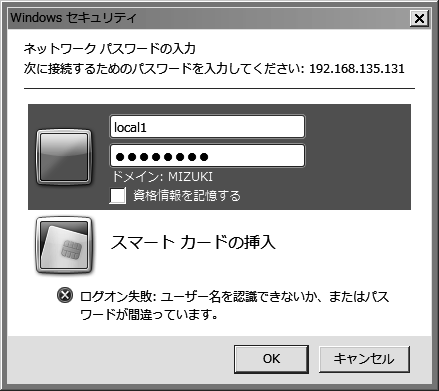
\includegraphics[width=.5\hsize]{image201304/samba/monyo-samba03_mono.png}
 \caption{ユーザー名とパスワードの入力ダイアログ}
 \label{fig:monyo-samba03.png}
\end{center}
\end{figure}

先ほど設定したuser1というユーザ名とパスワードを入力すれば、user1というホームディレクトリの共有と{\tt{tmp-share}}という先ほど作成した共有が見えているはずです(図\ref{fig:monyo-samba04.png})。

% --- samba04.png ---%
\begin{figure}[h]
\begin{center}
 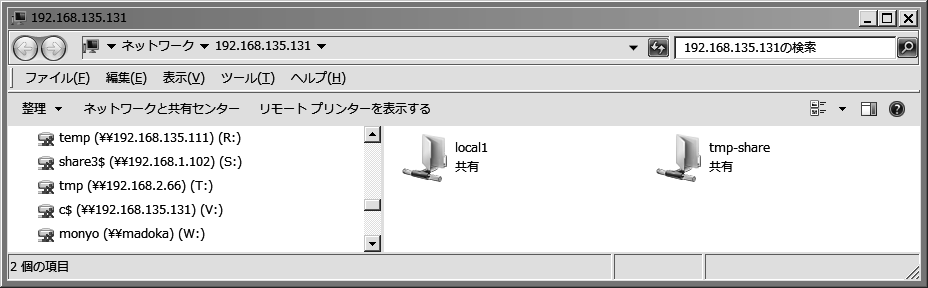
\includegraphics[width=0.8\hsize]{image201304/samba/monyo-samba04_mono.png}
 \caption{エクスプローラーからSambaサーバの共有を参照}
 \label{fig:monyo-samba04.png}
\end{center}
\end{figure}

\subsection{SambaをActive Directory(Windowsドメイン)に参加させてみる}

次に、SambaをActive Directoryに参加させて、先ほど構築したファイルサーバへのアクセスの際の認証をWindowsドメインに統合してみましょう。これもパッケージを適切にインストールしていれば簡単です。

まず次のようにして{\tt{/etc/resolv.conf}}を編集して、DNSドメイン、DNSサーバとしてActive DirectoryのDNS サーバを指定します(まだ指定していない場合) 。ここではW2K8R2AD3.LOCALというドメイン名でDNSサーバのIPアドレスが192.168.135.100である場合の例を示します(DHCPからIPアドレスを取得する設定の場合、このファイルは上書きされてしまうので、固定IPの設定にしておく必要があります):

\begin{commandline}
domain w2k8r2ad3.local ← Active Directory のドメイン名を指定
search w2k8r2ad3.local
nameserver 192.168.1.100 ← Active Directory の DNS サーバ (通常はドメインコントローラ) の IP アドレスを指定
\end{commandline}

ついで、{\tt{smb.conf}}ファイルを修正します。ここではW2K8R2AD3.LOCALというActive Directoryドメインに参加させる場合を例に取って説明します。

\begin{commandline}
[global]
  ...

  workgroup = W2K8R2AD3

  ...

  security = ads
  realm = W2K8R2AD3.LOCAL
\end{commandline}

最後に、{\tt{net ads join}}コマンドを使ってSambaをドメインに参加させます

\begin{commandline}
# net ads join -U administrator
Enter administrator's password:
Using short domain name -- W2K8R2AD3
Joined 'SQUEEZE32-5' to realm 'W2K8R2AD3.local'
No DNS domain configured for squeeze32-5. Unable to perform DNS Update.
DNS update failed!
\end{commandline}

{\tt{-U}}オプションに続き、ドメイン参加に使用するユーザを指定します。これは必ずしもAdministratorである必要はありませんが、Active Directory側の設定に依存しますので、事前に確認していてください。参加の際、DNS update failed! というエラーが出ますが、これは無視して構いません。

次に、このサーバへのアクセスを行うユーザを作成します。認証はActive Directoryで行うので、Sambaユーザは不要です。{\tt{/etc/passwd}}にユーザを追加します。このユーザのユーザ名はActive Directory側と合わせる必要があります。ここでは Active Directory 側にaduser01というユーザが既に作成済である前提で、aduser01を追加して見ます:

\begin{commandline}
# useradd -m aduser01
\end{commandline}

ここで次のようにしてSambaサーバを再起動して{\tt{smb.conf}}の設定変更を反映させます。

\begin{commandline}
# /etc/init.d/samba restart
Stopping Samba daemons: nmbd smbd.
Starting Samba daemons: nmbd smbd.
\end{commandline}

再起動後、Windows側にaduser01としてログオンの上、{\yen}{\yen}{\sf{Samba}}{\gt{サーバの}}{\sf{IP}}{\gt{アドレス}}としてWindowsからアクセスしてみましょう。認証を聞かれることなく、Sambaサーバにアクセスできるはずです。何かファイルを作成の上Debian上で確認すると、次のようにファイルの所有者がaduser01になっていることが確認できると思います。

\begin{commandline}
# ls -l
total 4
drwx------ 2 root     root     4096 Apr 14 11:24 ssh-XHMOEq1038
-rwxr--r-- 1 aduser01 aduser01    0 Apr 14 11:22 test01.txt
\end{commandline}

Active Directory 参加前との簡単な比較を図\ref{fig:monyo-winbind0.eps}に示します:

\begin{figure}[h]
\begin{center}
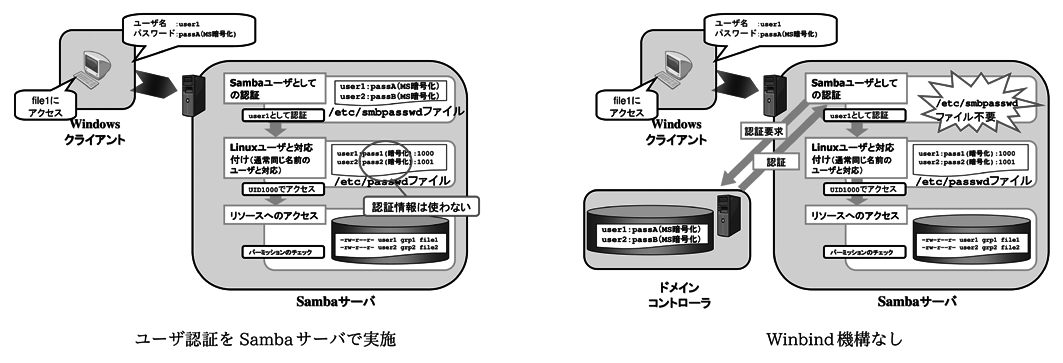
\includegraphics[width=1\hsize]{image201304/samba/monyo-winbind0_mono.png}
\end{center}
\caption{Active Directory参加前後の認証フローの比較}
\label{fig:monyo-winbind0.eps}
\end{figure}

\subsection{ユーザの作成を自動化する}

ここまでの設定で、認証の統合には成功しました。しかしこの状態だと認証を行いたいユーザ毎にDebian上の{\tt{/etc/passwd}}にユーザを作成する必要があります。多数のユーザがアクセスする必要がある環境では、ユーザのメンテナンスがかなりの負荷になってしまうと思います。

Sambaでは{\bf{Winbind}}という機能を使うことで、ユーザの自動生成が可能になります。パッケージを使っていれば、この設定も簡単に行えます。

まず、次のようにしてwinbindパッケージをインストールします:

\begin{commandline}
# apt-get install winbind
\end{commandline}

{\tt{wbinfo -t}}コマンドを用いて、次のようにRPCが成功することを確認しておきましょう:

\begin{commandline}
# wbinfo -t
checking the trust secret for domain W2K8R2AD1 via RPC calls succeeded
\end{commandline}

引き続き、{\tt{/etc/nsswitch.conf}}の{\tt{passwd:}}および{\tt{group:}}行に、次のように{\tt{winbind}}というキーワードを追加します:

\begin{commandline}
passwd:         compat winbind
group:          compat winbind
\end{commandline}

最後に、{\tt{smb.conf}}内の次の行のコメントを外し、設定を追加して、winbindを再起動します:

\begin{commandline}
# Some defaults for winbind (make sure you're not using the ranges
# for something else.)
   idmap uid = 10000-20000
   idmap gid = 10000-20000
   template shell = /bin/bash
   template homedir = /home/%U
\end{commandline}

ここでActive Directoryに例えばaduser02というユーザを追加して、その情報を取得すると$\cdots \cdots$

Sambaサーバの{\tt{/etc/passwd}}では特にユーザの追加を行っていないにも関わらず、次のようにWinbind機構によって自動生成されたユーザ情報が返却されるはずです:

\begin{commandline}
$ id 'W2K8R2AD3\aduser02'
uid=10001(W2K8R2AD3\aduser02) gid=10000(W2K8R2AD3\domain users) groups=10000(W2K8R2AD3\domain users)
$ getent passwd  'W2K8R2AD3\aduser02'
W2K8R2AD3\aduser02:*:10001:10000:aduser 02:/home/aduser02:/bin/bash
\end{commandline}

WindowsにユーザでログオンしてSambaサーバの共有に何かファイルを作成すると、次のように、ユーザ名、グループ名に自動生成されたものが表示されていることが確認できます:

\begin{commandline}
$ ls -l /tmp
total 4
drwx------ 2 root               root                   4096 Apr 14 12:40 ssh-wQPxWv1345
-rwxr--r-- 1               1001 aduser01                  0 Apr 14 11:22 test01.txt
-rwxr--r-- 1 W2K8R2AD3\aduser02 W2K8R2AD3\domain users    0 Apr 14 12:39 test02 - コピー.txt
\end{commandline}

Winbind機構のない状態とWinbind機構を有効にした状態での比較を次の図\ref{fig:monyo-winbind1.eps}に示します:

\begin{figure}[h]
\begin{center}
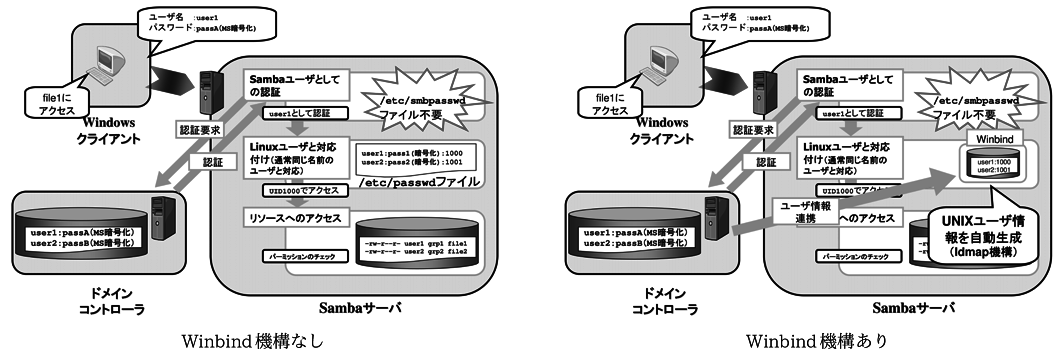
\includegraphics[width=1\hsize]{image201304/samba/monyo-winbind1_mono.png}
\caption{Winbind機構有無による認証フローの比較}
\label{fig:monyo-winbind1.eps}
\end{center}
\end{figure}

ここで自動生成されるユーザ、グループのUID,GIDやシェルなどの情報は、さまざまな設定でカスタマイズすることが可能です。今回は時間がないので省略しますが、1点だけ、生成されるユーザ名、グループ名に付加されるドメイン名部分が煩雑だと感じる場合は、{\tt{smb.conf}}に次のパラメータを設定してください。

\begin{commandline}
  winbind use default domain = yes
\end{commandline}

次のようにドメイン名がない単純な名前で表示されるようになります:

\begin{commandline}
$ id aduser02
uid=10001(aduser02) gid=10000(domain users) groups=10000(domain users)
\end{commandline}

ただし、当然ですがSambaが所属するドメインが他のドメインと信頼関係を結んでいるような複数ドメイン環境では名前が重複することがあります。

\subsection{sshの認証をWindowsに統合してみる}

ここまでの設定で、Sambaを用いる際のユーザ認証と、ユーザの自動作成について説明しました。最後にSamba以外のプロダクトからこのユーザ認証を活用する方法について説明します。ここではsshを例に取って説明しますが、PAMで認証を行うプロダクトであれば、同様の適用が可能です。

実は、ここまでの設定を行っていれば、Active Directoryのユーザを用いてLinuxにログインすることが(他の方法でログインを抑止していない限り)可能です。次に例を示します:

\begin{commandline}
$ ssh 192.168.135.35 -l W2K8R2AD3\\aduser02
W2K8R2AD3\aduser02@192.168.135.35's password:
Linux squeeze32-5 2.6.32-5-686 #1 SMP Mon Jan 16 16:04:25 UTC 2012 i686

The programs included with the Debian GNU/Linux system are free software;
the exact distribution terms for each program are described in the
individual files in /usr/share/doc/*/copyright.

Debian GNU/Linux comes with ABSOLUTELY NO WARRANTY, to the extent
permitted by applicable law.
Could not chdir to home directory /home/aduser02: No such file or directory
W2K8R2AD1\aduser02@squeeze32-5:/$
\end{commandline}

ホームディレクトリを作成していないため、エラーが発生していますが、ログイン自体は無事に成功していることが分かります。もちろんこのaduser02というユーザはWinbind機構によって自動作成されたものですので、{\tt{/etc/passwd}}上には存在していません。

ホームディレクトリがないと何かと不便ですが、手作業で作成するのもゲイがないので、最後にホームディレクトリを自動で作成する方法を紹介します。まず次のようにして{\tt{libpam-modules}}をインストールしてください:

\begin{commandline}
# apt-get install libpam-modules
\end{commandline}

その後、{\tt{/etc/pam.d/common-session}}ファイルに次のように 1 行追加します:

\begin{commandline}
session optional                        pam_winbind.so
# end of pam-auth-update config
session    required    pam_mkhomedir.so skel=/etc/skel/ umask=0022 ←この行を追加
\end{commandline}

オプションの詳細は{\tt{pam\_mkhomedir(8)}}を参照してください。

Debianでは{\tt{pam-auth-update}}というコマンドで自動的にPAMの設定を行う方法もありますが、残念ながら上記の設定はサポートしていないため、手作業でファイルを修正する必要があります。

設定後、先ほどと同様に別のマシンからaduser02でログインすると、次のようにCreating directory $\ldots$ というメッセージが表示されて、ホームディレクトリが自動作成されていることが確認できます:

\begin{commandline}
$ ssh 192.168.135.35 -l W2K8R2AD3\\aduser02
W2K8R2AD3\aduser02@192.168.135.35's password:
Creating directory '/var/home/aduser02'.
Linux squeeze32-5 2.6.32-5-686 #1 SMP Mon Jan 16 16:04:25 UTC 2012 i686

The programs included with the Debian GNU/Linux system are free software;
the exact distribution terms for each program are described in the
individual files in /usr/share/doc/*/copyright.

Debian GNU/Linux comes with ABSOLUTELY NO WARRANTY, to the extent
permitted by applicable law.
Last login: Sun Apr 14 11:40:23 2013 from 192.168.135.16
W2K8R2AD3\aduser02@squeeze32-5:~$
\end{commandline}

\dancersection{Ruby In Wheezy}{佐々木洋平}

\vspace{1em}

次期安定版 Debian 7.0 (Wheezy) における Ruby 環境について、%
特に複数の Ruby 実装の共存と Gem とのお付き合いの仕方について、
簡単にお話しします。
\index{ruby}

\subsection{``Ruby'' in Wheezy}

Ruby には複数の実装が存在しています。
Debian Wheezy では以下の Ruby インタープリタが使用できます:
\begin{table}[h!]
  \centering
  \begin{tabular}{lll}
    インタープリタ & パッケージ名       & 注意書き \\
    MRI 1.8.7      & \texttt{ruby1.8}   &          \\
    MRI 1.9.3      & \texttt{ruby1.9.3} & \texttt{ruby1.9.1} パッケージの実態は \texttt{ruby1.9.3} だったりします。 \\
    JRuby          & \texttt{jruby}     & パッケージは Debian Java Maintainers によって管理されています \\
    Rubinius       & \texttt{rubinius}  & 現在作業中です. ITP\#591817 \\
    mruby          & \texttt{mruby}     & 現在作業中です. ITP\#697835 \\
  \end{tabular}
\end{table}
%
\newline
「\texttt{ruby1.9.1} パッケージの実態は \texttt{ruby1.9.3} だったりします。」について、
Ruby の soname が変わっていないので \texttt{libruby1.9.1} 等のパッケージが残っており、
\texttt{ruby1.9.3} パッケージは \texttt{/usr/bin/ruby1.9.1} への
symbolic link を提供するだけだったりします。
\begin{commandline}
% dpkg -S ruby1.9.3
ruby1.9.3: /usr/bin/ruby1.9.3
ruby1.9.3: /usr/share/man/man1/ruby1.9.3.1.gz
ruby1.9.3: /usr/share/doc/ruby1.9.3
ruby1.9.3: /usr/share/doc/ruby1.9.3/NEWS.Debian.gz
ruby1.9.3: /usr/share/doc/ruby1.9.3/NEWS.gz
ruby1.9.3: /usr/share/doc/ruby1.9.3/changelog.Debian.gz
ruby1.9.3: /usr/share/doc/ruby1.9.3/changelog.gz
ruby1.9.3: /usr/share/doc/ruby1.9.3/copyright
ruby1.9.3: /usr/share/doc/ruby1.9.3/README.gz
% ls -la /usr/bin/ruby1.9.3
lrwxrwxrwx 1 root root 9 Feb 23 23:44 /usr/bin/ruby1.9.3 -> ruby1.9.1*
\end{commandline}
他にも、\texttt{Topaz} や \texttt{HPC Ruby Compiler} など、(個人的に)気になる実装がありますが、まだ Debian でどうこうというお話にはなっていません。

\subsection{複数の Ruby 実装の切り替え}

さて、これだけ複数の Ruby 実装があると、それを切り替えて使いたくなるのが人情だと思います。
Debian には、同じ機能を提供するソフトウェアをきりかえる \texttt{update-alternatives} という仕組みが既にあります。
ですが、\texttt{/usr/bin/ruby} を切り替えたら \texttt{gem} や \texttt{irb} なんかも切り替えたくなるでしょう。
そのため、これらを一度に変換するためのコマンドが提供されています。

\subsubsection{システム全体でデフォルトの Ruby を切り替えるには?: \texttt{ruby-switch}}

システム全体でデフォルトの Ruby インタープリタを選択するために、ruby-switch パッケージが使用可能です。 これは root として(もしくは sudo を使って)実行する必要があります。
\begin{commandline}
# ruby -v
ruby 1.8.7 (2011-06-30 patchlevel 352) [x86_64-linux]
# ruby-switch --list
ruby1.8
ruby1.9.1
# ruby-switch --set ruby1.9.1
update-alternatives: using /usr/bin/gem1.9.1 to provide /usr/bin/gem (gem) in manual mode.
update-alternatives: using /usr/bin/ruby1.9.1 to provide /usr/bin/ruby (ruby) in manual mode.
# ruby -v
ruby 1.9.3p0 (2011-10-30 revision 33570) [x86_64-linux]
# ruby-switch --auto
update-alternatives: using /usr/bin/ruby1.8 to provide /usr/bin/ruby (ruby) in auto mode.
update-alternatives: using /usr/bin/gem1.8 to provide /usr/bin/gem (gem) in auto mode.
# ruby -v
ruby 1.8.7 (2011-06-30 patchlevel 352) [x86_64-linux]
\end{commandline}

\subsubsection{ユーザ毎にデフォルトの Ruby インタープリタを選択するには: \texttt{rbenv}}

ユーザアカウント毎にデフォルトの Ruby インタープリタを切り替えるには、rbenv パッケージを使うのが良いでしょう。
\begin{commandline}
% ruby -v
ruby 1.8.7 (2011-06-30 patchlevel 352) [x86_64-linux]
% rbenv init
# Load rbenv automatically by adding
# the following to ~/.bash_profile:

eval ``$(rbenv init -)"
% echo 'eval ``$(rbenv init -)"' >> ~/.bash_profile # or ~/.bashrc, depends on your setup
% rbenv versions
% rbenv alternatives
% rbenv versions
  1.8.7-debian
  1.9.3-debian
% rbenv global 1.9.3-debian
% ruby -v
ruby 1.8.7 (2011-06-30 patchlevel 352) [x86_64-linux]
\end{commandline}
%%$
一見ちゃんと動作していないように見えますが、これは現在実行中のシェルが "ruby" の位置として /usr/bin/ruby をキャッシュしているからです。新しいシェルを開始した後には、デフォルトの Ruby を行ったり来たり切り替えることができます。
\begin{commandline}
% ruby -v
ruby 1.8.7 (2011-06-30 patchlevel 352) [x86_64-linux]
% rbenv global 1.9.3-debian
% ruby -v
ruby 1.9.3p0 (2011-10-30 revision 33570) [x86_64-linux]
% rbenv global 1.8.7-debian
% ruby -v
ruby 1.8.7 (2011-06-30 patchlevel 352) [x86_64-linux]
\end{commandline}

\subsubsection{Debian パッケージになっていない Ruby をインストールするには: \texttt{ruby-build}}

\texttt{ruby-build} を使用することで、Debian でまだ使用可能になっていない Ruby インタープリタをインストールすることができます。
しかしながら、このパッケージの README.Debian ファイルに書かれている内容に注意して下さい:
\begin{commandline}
  While ruby-build is a great tool to build Ruby versions that are not
  available via APT, you should still use the Debian-packaged versions
  of Ruby whenever possible since they are tested and supported by the
  Debian community.

  Please do not report bugs you encounter while using your homebuilt
  Rubies to the Debian team; Rubies built by yourself are not supported.
\end{commandline}
% とはいえ \texttt{ruby2.0} がそろそろ出ますし、\texttt{ruby-build} を使う人も多いと思います.
% \footnote{個人的には \texttt{backports} する予定ですが.}.
というわけで、詳細は \texttt{man ruby-build} ということで。

\subsection{Debian における Ruby パッケージング}

Debian では Ruby 本体のパッケージングは \texttt{pkg-ruby} チーム、
Gem 等で配布されている(拡張)ライブラリやアプリケーションは
\texttt{pkg-ruby-extras} チームによってメンテされています。
次の話題は
\texttt{pkg-ruby-extras} チームが良くやっていること、
すなわち Gem で配布されている Ruby (拡張)ライブラリの Debian パッケージ化について、です。

\subsection{Gem パッケージを Debian パッケージに: \texttt{gem2deb}}

Gem で配布されている Ruby (拡張)ライブラリは
\texttt{gem2deb} を用いることで Debian パッケージに変換可能です。\textbf{たいていの場合は}。
\texttt{gem2deb} によるお手軽パッケージングの成功率は perl の\texttt{dh\_make\_perl}
\footnote{%
  CPAN にある perl ライブラリ/モジュールを Debian パッケージにするコマンド
}
ぐらい、だと思って下さい(もっと低いかも)。

たとえば \texttt{hogehoge} という gem を Debian パッケージにしたい場合には
\begin{commandline}
% sudo apt-get install gem2deb
...
% gem fetch hogehoge
...
% gem2deb hogehoge[version].gem
...
% sudo dpkg -i ruby-hogehoge_[version].deb
\end{commandline}
で良い筈です。
ちなみにこれらは MRI 1.8.7, MRI 1.9.3 向けのパッケージとなります。

%\subsection{まとめ...?}
%
%当日の demo をふまえて、後日加筆修正する予定です。

%201303tokyo
%-------------------------------------------------------------------------------
\dancersection{gdb python拡張その1}{野島 貴英}
%-------------------------------------------------------------------------------
%$

\index{gdb-pythonかくちょう@gdb-python拡張}
\subsection{はじめに}

 Debianパッケージのバイナリのバグ潰しを行う時、gdbなどのデバッガを使ってデバッグを
する事も多いかと思います。しかしながら、プログラムの構造が大規模/複雑になってくると、
デバッグ作業も大変になっていきます。また、プログラムについても、
抽象化が激しく行われていると、デバッガ無しには解析が非常に困難かと思います。

\index{gdb}
 gdbはv7.0からpython拡張が搭載されており
\footnote{\url{http://ftp.gnu.org/gnu/gdb/}調べ}、gdbをpythonスクリプトで操る
事ができます。こちらを利用する事により、人手では、工数かかりすぎでなかなか
進まなかったデバッグも可能になっていくと思います。

 今回は、gdbのpython拡張の一部を説明し、最後はC言語で作られた
プログラムの実行トレースを実際にpython拡張機能を用いて、取得してみる
ところまでやってみます。

\subsection{Debian sidのgdb python拡張の基本情報}

 debian sidに含まれているgdbは最初からpython拡張が有効にしてあるようです。
表\ref{tab:gdb-python-basic-info}に基本情報を載せます。

\begin{table}[ht]
\begin{center}
\small
\begin{tabular}{|l|l|l|}
\hline
項番 & 項目 & 値 \\
\hline
1 & gdbバージョン & 7.4.1 \\
2 & pythonバージョン & 2.7.3 \\
3 & pythonサーチパス & /usr/share/gdb/python,/usr/lib/python2.7以下 \\
\hline
\end{tabular}
\caption{Debian sid環境に含まれるgdbとpythonの基本情報}
\label{tab:gdb-python-basic-info}
\end{center}
\end{table}

 今回はdebian sid amd64環境でテストした結果を元に説明を行います。

\subsection{python拡張を簡易的に動かしてみる}

 gdbよりpython言語を簡易的に呼び出す場合、gdbのコマンドラインから接頭辞として
pythonをつけて起動します。また、gdbコマンドラインから
pythonのみを指定すると、Ctrl+dを押下するまで、複数のpython構文を
指定できます。(なお、Ctrl+dを押下すると、gdbのコマンドラインに復帰する
と同時に入力した複数のpython構文が一度に評価されます)

 なお、pythonで一度定義した変数などはgdbを終了するまで何度でも
参照できます。

\begin{commandline}
$ gdb 
GNU gdb (GDB) 7.4.1-debian
Copyright (C) 2012 Free Software Foundation, Inc.
...中略...
For bug reporting instructions, please see:
<http://www.gnu.org/software/gdb/bugs/>.
(gdb) python print "hello world"
hello world
(gdb) python a=[1,2,3,4]
(gdb) python print a
[1, 2, 3, 4]
(gdb) python a.append(5)
(gdb) python print a
[1, 2, 3, 4, 5]
(gdb) python
>import sys
>print sys.path
>print sys.version_info
>ここでCtrl+d
['/usr/share/gdb/python', '/usr/lib/python2.7',
  '/usr/lib/python2.7/plat-linux2', '/usr/lib/python2.7/lib-tk',
  '/usr/lib/python2.7/lib-old', '/usr/lib/python2.7/lib-dynload',
  '/usr/local/lib/python2.7/dist-packages',
  '/usr/lib/python2.7/dist-packages',
  '/usr/lib/python2.7/dist-packages/PIL',
  '/usr/lib/python2.7/dist-packages/gst-0.10',
  '/usr/lib/python2.7/dist-packages/gtk-2.0',
  '/usr/lib/pymodules/python2.7']
sys.version_info(major=2, minor=7, micro=3, releaselevel='final', serial=0)
\end{commandline}
% $ 
\subsection{gdbのpython拡張の構造}

 gdbのpython拡張は図\ref{fig:python-internal-schema}のような構造となっています。

\begin{figure}[h]
\begin{center}
 \includegraphics[width=0.8\hsize]{image201301/gdb-python/gdb-python-internal-schema.eps}
 \caption{gdbとpython拡張の構造}
 \label{fig:python-internal-schema}
\end{center}
\end{figure}

\subsection{module gdbのマニュアル}

 gdb本体にmodule gdbが実装されているため、module gdbの
pythonドキュメントについては、gdb上でpythonからhelp(gdb)を呼び出す必要
があります。

 以下に読み方を示します。なお、以降、(gdb)はgdbのプロンプトを示します。

\begin{commandline}
(gdb) python help(gdb)
Help on package gdb:

NAME
    gdb

FILE
    (built-in)

PACKAGE CONTENTS
    command (package)
    printing
    prompt
    types

...中略...
\end{commandline}

 また、gdbのpython拡張についてのさらに詳しい説明は、info gdbにて
Extending GDB→pythonの項目から参照できます。

\subsection{module gdbに定義されているオブジェクト群}

 図\ref{fig:python-class-schema-1}〜図\ref{fig:python-class-schema-2}に、
module gdbに定義されているオブジェクト群のclass図を載せます。

 gdb拡張用のpythonスクリプトを記載する場合、これらオブジェクトを併用して
gdbとのデータのやりとり、あるいは、操作を行います。

\begin{figure}[h]
\begin{center}
 \includegraphics[width=0.8\hsize]{image201301/gdb-python/gdb-python-class-schema-1.eps}
 \caption{module gdbのclass図(その1)}
 \label{fig:python-class-schema-1}
\end{center}
\end{figure}

\begin{figure}[h]
\begin{center}
 \includegraphics[width=0.8\hsize]{image201301/gdb-python/gdb-python-class-schema-2.eps}
 \caption{module gdbのclass図(その2)}
 \label{fig:python-class-schema-2}
\end{center}
\end{figure}

\newpage

\subsection{gdbのコマンドを増やしてみる}

 gdbのpython拡張は柔軟な機能を持つため、いろいろな使い方ができます。
ここでは、試しにgdbのコマンドを増やしてみます。

 gdbのコマンドをpythonから増やすには、gdb.commandクラスを継承したクラスを
用意し、gdb.command.\_\_init\_\_()にてコマンド名と共に登録する事により行います。

 info gdbのExtending GDB→Python→Python API→Commands In Pythonに
記載されている方法を試して、hello-worldコマンドを登録してみます。

\begin{commandline}
-----hello.pyの中身ここから-----
# -*- coding: utf-8 -*-
# coding:utf-8
import gdb
class HelloWorld (gdb.Command):
  """ Greet the whole world """
  def __init__ (self):
     super(HelloWorld, self).__init__ ("hello-world",gdb.COMMAND_OBSCURE)

  def invoke (self,arg, from_tty):
     print "Hello, World! arg=["+str(arg)+"]"

HelloWorld()
-----hello.pyの中身ここまで-----
\end{commandline}

 追加したコマンドについていろいろ実行してみます。

\begin{commandline}
(gdb) source hello.py
(gdb) hello-[ここでTABを押すと補完される]
(gdb) hello-world foo,bar,com
Hello, World! arg=[foo,bar,com]
(gdb) help obscure
Obscure features.

List of commands:

...中略...
hello-world --  Greet the whole world 
...中略...
\end{commandline}

 コマンド hello-worldが追加されています。また、引数はinvoke()のargに文字列として
まとめて入ります。また、コマンドカテゴリのOBSCUREに登録されている事がhelp obscure
にて判ります。

\subsection{作ったpythonスクリプトを自動で読み込ませるには}

 ところで、gdbのpython拡張を理解するにつれ、高度なデバッグ用スクリプトを用意するように
なってくると思います。すると、作ったpythonスクリプトをいつもgdbに自動で読み込ませ
ておきたくなるかと思います。方法としては、以下の3つの方法があります。

\subsubsection{\$\{HOME\}/.gdbinitを使う方法}

 以下のようなファイルを\verb!${HOME}/.gdbinit!に記載しておきます。

\begin{commandline}
----${HOME}/.gdbinitここから-----
source /home/foo/bar/my-gdb-func.py
----${HOME}/.gdbinitここまで-----
\end{commandline}

こうすると、\verb!${HOME}!にホームディレクトリがあるようなユーザがgdbを起動した時に、
自動的に/home/foo/bar/my-gdb-func.pyがロードされて評価されるようになります。

\subsubsection{セクション名:.debug\_gdb\_scriptsを使う方法}

 バイナリ形式によりますが、任意のセクション名を持つ事が可能なバイナリ形式
(例:ELF,DWARF)にて、.gdb\_gdb\_scriptsセクションを作成し、ここにスクリプト名
を打ち込んでおく事ができる場合があります。この場合、カレントディレクトリにある、
同名のスクリプトをgdbが自動的にロードしてくれます。
なお、本機能は、gdb変数のauto-load-scriptがonの時に有効です(デフォルトはon。)

 以下に例を示します。ここでは先ほどのhello.pyを自動でロードするように
asm\{\}命令で.debug\_gdb\_scriptsセクションを直接指定しています。

\begin{commandline}
------hello.cの中身ここから------
#include <stdio.h>

asm(
".pushsection \".debug_gdb_scripts\",\"MS\",@progbits,1\n"
".byte 1\n"
".asciz \"hello.py\"\n"
".popsection \n"
);

int main(int argc,char **argv)
{
        printf("hi there!");
        return 0;
}
------hello.cの中身ここまで------

実行結果:
$ gcc -o hello hello.c
$ ls 
hello hello.py hello.c
$ gdb hello
GNU gdb (GDB) 7.4.1-debian
Copyright (C) 2012 Free Software Foundation, Inc.
...中略...
<http://www.gnu.org/software/gdb/bugs/>...
Reading symbols from /home/xxxx/hello...done.
(gdb) info auto-load-scripts
Loaded  Script                                                                 
Yes     hello.py                                                         
	full name: /home/xxxx/hello.py
(gdb) hello-world 
Hello, World! arg=[]
\end{commandline}
%$

\subsubsection{``バイナリ名''-gdb.pyをスクリプト名に使う方法}

 ファイル名として、``バイナリ名''-gdb.pyをファイル名に持つpythonスクリプトを
カレントディレクトリに置いておくと、gdbがバイナリ名のファイルをロードした時、
自動でロードしてくれます。なお、本機能は、gdb変数のauto-load-scriptがonの時に
有効です(デフォルトはon)

 以下の例では、gdb helloとすると、無事先ほどのhello.pyが読み込まれ、
hello-worldコマンドが登録されている事がわかります。

\begin{commandline}
------hello.cの中身ここから------
#include <stdio.h>

int main(int argc,char **argv)
{
        printf("hi there!");
        return 0;
}
------hello.cの中身ここまで------

コンパイル:
$ gcc -o hello hello.c
$ mv hello.py hello-gdb.py (←先ほどのhello.pyの名前を"バイナリ名"-gdb.pyへ変更)
$ ls 
hello hello-gdb.py hello.c
$ gdb hello
GNU gdb (GDB) 7.4.1-debian
Copyright (C) 2012 Free Software Foundation, Inc.
...中略...
<http://www.gnu.org/software/gdb/bugs/>...
Reading symbols from /home/xxxx/hello...done.
(gdb) info auto-load-scripts
Loaded  Script                                                                 
Yes     /home/xxxx/hello-gdb.py
(gdb) hello-world 
Hello, World! arg=[]
\end{commandline}
%$

\subsection{break/finishと応用例について}

 デバッガの基本機能にbreakpointがあります。こちらの機能を
pythonから利用するには gdb.Breakpoint class及び、
gdb.FinishBreakpoint classを継承する事により行います。
これらclassを用いれば、gdbのbreak/watch/finishコマンドを独自拡張できます。

 ここでは、応用としてバイナリ内部の関数呼び出しの記録を取るようなpythonスクリプト
を書いてみます。

\begin{commandline}
-------calltracer.pyここから---------
# -*- coding: utf-8 -*-
# coding:utf-8
import gdb
class _CallTracerFinishBreakpoint(gdb.FinishBreakpoint):
	def __init__(self, name, stack):
		super(_CallTracerFinishBreakpoint, self).__init__(internal=True)
		self._stack_ptr=stack
		self._name=name
		self.silent=True
	def stop(self):
		print (" " * (len(self._stack_ptr)))+"<="+self._name
		self._stack_ptr.pop()
		return False
	def out_of_scope(self):
		print "Abnormal jump out frame"
		print (" " * (len(self._stack_ptr)))+"<="+self._name
		self._stack_ptr.pop()
		return False

class _CallTracerBreakpoint(gdb.Breakpoint):
	def __init__(self, spec, name, stack):
		super(_CallTracerBreakpoint, self).__init__(spec, 
							    gdb.BP_BREAKPOINT,
							    internal = False)
		self._stack_ptr=stack
		self._name=name
		self.silent=True
	def stop(self):
		self._stack_ptr.append(self._name)
		print (" " * (len(self._stack_ptr)))+"=>"+self._name
		try:
			_CallTracerFinishBreakpoint(self._name, self._stack_ptr)
		except:
			print "uh? cant put finish break on "+self._name
		return False

class _ReAnalyzeCallTracer(gdb.Command):
	""" reanalyze symbol for calltracer """
	def __init__(self):
		super(_ReAnalyzeCallTracer, self).__init__('reanalyzecalltracer',
							gdb.COMMAND_OBSCURE)
		self._stack=[]
	def _retrive_ptrs(self):
		info=gdb.execute("info break",False, True)
		info_lines=info.splitlines()
		ptrs={}
		for idx in range(0,len(info_lines[1:])):
			tokens=info_lines[idx+1].split()
			if len(tokens) > 5:
				if ptrs.has_key(tokens[4]) == False:
					ptrs[tokens[4]]=" ".join(tokens[5:])
		return ptrs
	def invoke(self, arg, from_tty):
		break_info=self._retrive_ptrs()
		gdb.execute("delete",False, True)
		gdb.execute("set pagination off")
		for addr,name in break_info.iteritems():
			_CallTracerBreakpoint(r'*'+addr,
					      name,self._stack)
_ReAnalyzeCallTracer()

class _PrepareCallTracer(gdb.Command):
	""" prepare call tracer for c """
	def __init__(self):
		super(_PrepareCallTracer, self).__init__('prepcalltracer',
							 gdb.COMMAND_OBSCURE)
	def invoke(self, arg, from_tty):
		gdb.execute("rbreak",False, True)
		gdb.execute("reanalyzecalltracer",False, True)
		print "prepare done!"

_PrepareCallTracer()
-------calltracer.pyここまで---------
-------デバッグ対象:chkfunc.c ここから-------
#include<stdio.h>

void foo_a(const char *str)
{
	printf("%s\n",str);

}
void caller_bar(void)
{
	foo_a("caller is bar!");
}
int main(int argc,char **argv)
{
	foo_a("caller is main!");
	caller_bar();
	return(0);
}
-------デバッグ対象:chkfunc.c ここまで-------
\end{commandline}
\begin{commandline}
実行結果:
$ gcc -O0 -g -o chkfunc chkfunc
$ ls
chkfunc.c chfunc calltracer.py
$ gdb ./chkfunc
GNU gdb (GDB) 7.4.1-debian
Copyright (C) 2012 Free Software Foundation, Inc.
...中略...
Reading symbols from /home/foo/bar/chkfunc...done.
(gdb) source calltracer.py
(gdb) prepcalltracer 
prepare done!
(gdb) run
Starting program: /home/foo/bar/chkfunc 
 =><_start>
uh? cant put finish break on <_start>
  =><__libc_start_main@plt>
   =><__libc_csu_init>
    =><_init>
     =><call_gmon_start>
     <=<call_gmon_start>
    <=<_init>
    =><frame_dummy>
     =><register_tm_clones>
     <=<frame_dummy>
    <=<register_tm_clones>
   <=<__libc_csu_init>
   =>in main at chkfunc.c:21
uh? cant put finish break on in main at chkfunc.c:21
    =>in foo_a at chkfunc.c:12
     =><puts@plt>
caller is main!
     <=<puts@plt>
    <=in foo_a at chkfunc.c:12
    =>in caller_bar at chkfunc.c:17
     =>in foo_a at chkfunc.c:12
      =><puts@plt>
caller is bar!
      <=<puts@plt>
     <=in foo_a at chkfunc.c:12
    <=in caller_bar at chkfunc.c:17
    =><__do_global_dtors_aux>
     =><deregister_tm_clones>
     <=<deregister_tm_clones>
    <=<__do_global_dtors_aux>
    =><_fini>
    <=<_fini>
[Inferior 1 (process 6413) exited normally]
Abnormal jump out frame
   <=<__libc_start_main@plt>
warning: Error removing breakpoint -5
(gdb)
\end{commandline}
%$

無事、バイナリ内部の関数呼び出しの記録が取れているかと思います。

\subsection{終わりに}

 今回gdbのpython拡張のいくつかを紹介してみました。pythonを
用いる事で、いろいろなデバッグ手法が取れるかと思います。

 次回は、Frame class/Value class等の応用について紹介したいと思います。

\begin{thebibliography}{98}
\bibitem{infogdb} Free Software Foundation, ``info gdb''
\bibitem{gdbpytutor} ``PythonGdbTutorial'',\url{http://sourceware.org/gdb/wiki/PythonGdbTutorial}
\bibitem{gdbpytest} Free Software Foundation, \verb!$(GDBSRC)/gdb/testsuite/gdb.python!以下のテスト用ファイル群
\end{thebibliography}

%201212tokyo
%-------------------------------------------------------------------------------
\dancersection{日本におけるDFSGの求める自由と2012年改正著作権法}{上川 純一}
%-------------------------------------------------------------------------------
\index{dfsg}
\index{ちょさくけんほう@著作権法}

\subsection{はじめに}

Debian の基本的な思想ともいえる Social Contract、およびその中に含まれる
DFSG は自由にソフトウェアの開発ができる環境を理想と考えるものです。ユーザ
を尊重するよりまえに100%フリーソフトウェアであることをうたっている点
などもあり、ソフトウェアの複製や改変をする自由を尊ぶユーザがDebianを選択
しています。

しかし自由なソフトウェアの開発は自明に支持されるものではありません。
自由なライセンスのソフトウェアを確保することは難しく、改変不自由な秘密のソフトウェアを買ってくるのは簡単です。
各国においての法律、企業による技術的設計・制約などに影響されます。

ソフトウェアを自由に勉強して改変して開発できる環境がないとソフトウェア利
用の幅が失われるだけでなく、
ソフトウェア開発できる人の層が薄くなり、結果として日本国におけるソフトウェ
ア開発能力の低下に至るでしょう。

自分で書いたソフトウェアを動かせないハードウェアしか市場にでまわってない
のであれば、ソフトウェアを作成するという経験を享受する機会が極端に減ります。

一年の棚卸の意味も兼ねて、最近の日本の事情を調べてみました。

\subsection{著作権法改正}

最近大きな法律の変化としては、2012年の改正著作権法があります。
議論の経緯や結果どういうことになったのか、などいろいろな情報が提供されているようなので
我々のソフトウェア開発にどういう影響がありそうか眺めてみました。

リッピングソフトやマジコンが規制対象になったと報道されていますが、具体的
にはどう変わったのでしょうか。
文化庁のウェブサイトにある解説\cite{bunka-chosaku2012}によると「(4)著
作権等の技術的保護手段に係る規定の整備」にあたるようです。
暗号の解読をともなう複製行為は民事上違法になり、
暗号の解読をできる装置やプログラムの譲渡などを行ったものに刑事罰(非親告
罪)が規定されました。

アメリカで成立して一時期大騒ぎになったDMCA 法というのがありました。 DMCA
でソフトウェア開発に影響の有りそうな部分も順次日本の著作権法に取り入れら
れているようです。 今回の著作権法改正では DRM を実装している暗号の解読す
るためのソフトウェアの作成が問題となっているようです。フリーソフトウェア
では DVD の再生に必要な鍵のライセンスが手に入らないため暗号を解読してしま
う(DeCSS)を利用するなどの回避策がとられてきました。海賊行為に流用できる
ということで業界には睨まれていたのですが、DRMを回避し複製できるソフトウェ
アの配布について刑事罰が設定されたようです。
\index{dmca}
\index{decss}

具体的には私的使用の複製に「知って DRM 回避して複製した場合」 を例外第30条
の2の例外事項に追加したようです。

著作権法の特色として、民事だけでなく親告罪でありながら刑事罰が規定されている点です。
親告罪とは、被害者が告訴しないと公訴を提起できないもので、親告罪でなけれ
ば警察が適当に被疑者を捕まえることができるようです。

アメリカではDMCA法の影響でDeCSSが配布できないとなった時にはUsenet上で
DeCSSのソースコードがSPAMで投稿されたり、DeCSSのソースコードが印刷された
Tシャツを着ることが流行したりしました。日本も同様の祭りは起きるんでしょ
うか。

libdvdreadパッケージは\cite{libdvdread-css}libdvdcssを利用してCSSの復号化
とDVDビデオの再生ができるのですが知ってDRMの回避をしていることになると思
われます。ただ、複製するために利用できますが、私的に再生するだけであれば
私的使用の「複製」をしているわけではないので著作権法の範囲ではありません。
オープンソースソフトウェアだけでDVDの再生をするためにはハードウェアがDVD
復号化を行うか、ソフトウェアがDeCSSをする仕組みが必要になります。オープン
ソースソフトウェアがDVDの複製に利用できるかもしれないということで配布した
ものに刑事責任が発生するかもしれない、そういう国になったみたいですね。
\index{libdvdread}

テレビのデジタル放送をオープンソースソフトウェアだけで視聴しようとすると
friio などのハードウェア機器を活用することになると思いますが、それもまた
検討が必要なのかもしれません。

\subsection{ハードウェア・ソフトウェアの傾向}

別に日本に限った話ではないのですが最近の気になる傾向なのでついでにまとめ
ておきました。

\subsubsection{セキュアブート}

最近は公開暗号方式で保護されているプラットフォームが増えてきました。
昔はゲームハードウェア、Nintendo DSなどが鍵を解読しないとソフトウェアを
動かせないというので有名でしたが、最近はAndroid携帯が署名されたファーム
ウェアしか起動しない、「セキュアブートに」対応しているOSがEFI経由適切に
署名されたOSしか起動しないという状況になっています。

iPhone などでは Jail break という方法が編み出され、セキュリティーホール
をついて自由にソフトウェアを改変して利用しているようです。いつまでも簡単
にセキュリティーホールが見つかるという保証はないので、難しい問題です。

\subsubsection{デバイスドライバとバイナリブロブ}

ハードウェアは一般にはオープンソースソフトウェア専用として開発しているも
のではなく、また激しい競争のある業界ではお互いにできるだけ多くの部分を秘
密にしておきたい。オープンソースのOSでもデバイスドライバのパラメータやロ
ジックなどはできるだけファームウェアとして秘密にしておきたい。下手に改変
されて法令準拠できない危険な改変ができないようにしたい\footnote{例えば無
線通信関連}。そういう要求を満たすためにデバイスドライバの多くの部分をユー
ザ(競合他社)の理解・改変できないバイナリ形式で提供するという慣習があり
ます。

デバイスドライバの秘密の部分をbinary blobと呼びDebianでは長年問題を検討し
てきました。KernelからBinary Blobを分離し、問題を露見し、かつ non-free で
Binary Blob を配布することでユーザに直接の不利益にならないようにしていま
す。

個人的にはリバースエンジニアリングについて論じてた委員会の論点がおもしろ
いと思いました。\cite{bunka-reverse-eng2008}相互運用のためのリバースエン
ジニアリングは著作権法の文面では著作権の範囲で保護されていないので、リバー
スエンジニアリングを利用者規定で禁止しているものが多いと思います。

\subsubsection{マーケット}

セキュアブートとの兼ね合いで重要になってくると思われる傾向ですが、Debian
Project自身もデフォルトではDebian Archive Keyで署名されたパッケージしか
インストールできないように設定されています。これはDebian Projectとして出
自がわかっている安全だと思われるファイルのみがインストールできるようにす
ることで誰でも間に介在できるインターネット経由でダウンロードしているとい
う環境で安全を担保する仕組みになっています。

現在最大規模だと思われる Apple Inc のアプリケーションマーケットではアッ
プルが規約に合致しているか審査してから配布許可を出すというシステムになっ
ています。iOS のハードウェアでは基本的にはAppleの許可したソフトウェアで
ないとインストールできなくなっています。規約でプログラム可能なソフトウェ
アというのを禁止しているので、iOSのハードウェアではプログラミングに親し
むことが難しくなっています。

\subsection{おわりに}

自由に技術研究できる文化と環境というのは既得権益を保護したい業界、もしくは激
しい競争の行われている業界で競合他社から秘密を守りたい業界の求める
変化の方向とは一致しません。
安全・安心・信頼できるなソフトウェアが欲しいという方向とも必ずしも一致しません。

一方に極端に有利な変更というのはそのまま通らないでしょうが、
一Debian ユーザーとして、自由なソフトウェア開発を支持する層として、今後
も状況を注視していきたいと思います。


\begin{thebibliography}{99}
 \bibitem{bunka-chosaku2012}
	 文化庁 「平成24年通常国会 著作権法改正について」
	 \url{http://www.bunka.go.jp/chosakuken/24_houkaisei.html}
 \bibitem{bunka-reverse-eng2008} 
	 文化審議会著作権分科会法制問題小委員会(第7回)議事録
	 「リバース・エンジニアリングに係る法的課題についての論点」
 \url{http://www.bunka.go.jp/chosakuken/singikai/housei/h20_07/shiryo_1.html}

 \bibitem{libdvdread-css}
	 libdvdread Debian package documentation
	 ``Content Scramble System (CSS)''
	 \url{/usr/share/doc/libdvdread4/README.css}

\end{thebibliography}

%201212kansai
\dancersection{月刊 Debian Policy「パッケージ管理スクリプトとインストールの手順」}{かわだ てつたろう}
\index{debian policy}

月刊 Debian Policy、今回読むのは第 6 章の「パッケージ管理スクリプトとインストールの手順」です。
この章ではパッケージをインストール、アップグレード、削除する際にパッケージ管理システムが走らせるスクリプトとその手順について説明されています。

さて、事前課題で内容は読んで理解していただいていると思いますのでざっと内容をみていきましょう。

\subsection{パッケージ管理スクリプト}
パッケージ管理スクリプトは次の 4 つの制御情報ファイルで、パッケージの一部として供給されます。

\begin{itemize}
\item preinst
\item postinst
\item prerm
\item postrm
\end{itemize}



\subsubsection{ファイル構成}
パッケージ管理スクリプトは実行可能ファイルでなければならず、ファイルのパーミッションは、誰でも読むことと実行可能でなければならないが誰でも書き込み可能ではいけない、{\tt 755} でなければいけません。
また、スクリプトであることが推奨されており、その場合は {\tt \#!} (shebang) で始まってなければなりません。

\subsubsection{終了ステータス}
パッケージ管理システムは終了ステータスコードを参照するので正しく終了ステータスコードを返すことが重要です。
処理が成功すれば 0 を、失敗すれば 0 以外を返さなければなりません。0 以外のステータスコードが返された場合、パッケージ管理システムはエラーと判断し以降の処理を停止します。

パッケージ管理スクリプトがシェルスクリプトなら常に {\it set -e} を使用する必要があります。

\subsubsection{PATH 環境変数}
{\tt PATH} 環境変数内から見つかることが期待できるプログラムは絶対パスで呼びだすべきではありません。
また、{\tt PATH} 環境変数はリセットすべきではありませんが、前後に付け加えることはかまいません。

\subsubsection{再入結果の同一性}
パッケージ管理スクリプトは、一度成功した処理を何度呼び出しても無害でなければならず、
失敗や中断した処理を再度呼び出しても前回の残された状態から実行しなければなりません。
いずれにせよ全ての処理が成功した場合にはパッケージ管理スクリプトは成功ステータスで終了しなければなりません。

これは、ひどく壊れたパッケージが残らないようにするためにとても重要です。

\subsubsection{パッケージ管理スクリプトからのターミナルの制御}
パッケージ管理スクリプトは、制御端末がある状態での実行が保証されていません。
ユーザとの対話ができない場合がありますので、非対話型で処理できるようにしなければなりません。

どうしても対話が必要な場合(優先順位が高く、妥当な標準回答がないなど)に制御端末が無ければパッケージ管理スクリプトは異常終了してもかまいません。
ただ、できるだけこのような状況は避けるべきです。たいていの場合、パッケージのバグと判断されます。

{\tt debconf} を用いる場合の詳細は「3.9.1 メンテナスクリプト中のプロンプト使用について」を参照してください。


\subsection{パッケージ管理スクリプトの呼ばれ方のまとめ}
パッケージ管理スクリプトがそれぞれ呼ばれるタイミングをおおまかにいうと次のようになります。

\begin{itemize}
\item preinst  … パッケージ展開前
\item postinst … パッケージ展開後
\item prerm    … パッケージ削除前
\item postrm   … パッケージ削除後
\end{itemize}

ここからは、パッケージ管理スクリプトのすべての呼ばれ方と、呼ばれる際に依存して良い機能についてのまとめです。
{\it new-} はインストール/更新/ダウングレード対象の新バージョンのパッケージから呼ばれるもの、
{\it old-} は更新/ダウングレードされる対象の旧バージョンのパッケージから呼ばれるものです。


\subsubsection{preinst}

\begin{itemize}
\item {\it new-preinst} install
\item {\it new-preinst} install {\it old-version}
\item {\it new-preinst} upgrade {\it old-version}
  \begin{itemize}
  \item パッケージは展開前
  \item essential パッケージと Pre-Depends パッケージのファイルのみがある
  \item Pre-Depends パッケージは展開された直後か Half-Configured の可能性がある
  \end{itemize}
\end{itemize}

\begin{itemize}
\item {\it old-preinst} abort-upgrade {\it new-version}
  \begin{itemize}
  \item アップグレードに失敗した場合に呼ばれる
  \item 展開されたファイルに依存してはいけない
  \item パッケージの依存関係は満たされていないかもしれない
  \item Pre-Depends は上記と同様
  \end{itemize}
\end{itemize}


\clearpage

\subsubsection{postinst}

\begin{itemize}
\item {\it postinst} configuire {\it most-recently-configured-version}
  \begin{itemize}
  \item パッケージと依存パッケージのファイルは展開されている
  \item 巡回依存関係になければ依存パッケージは設定されている
  \end{itemize}
\end{itemize}

\begin{itemize}
\item {\it old-postinst} abort-upgrade {\it new-version}
\item {\it conflictor's-postinst} abort-remove in-favour {\it package} {\it new-version}
\item {\it postinst} abort-remove
\item {\it deconfigured's-postinst} abort-deconfigure in-favour {\it failed-install-package} {\it version} [removing {\it conflicting-package} {\it version}]
  \begin{itemize}
  \item パッケージのファイルは展開されている
  \item 依存する全てのパッケージは少くとも Half-Installed 状態、完全に展開されていないこともある
  \item 依存関係が必要となる処理は実行するべきである、依存関係が満たされていないたいていの場合 {\tt postinst} を異常終了させるのがエラー処理を考慮すると適切な処理である
  \end{itemize}
\end{itemize}


\subsubsection{prerm}

\begin{itemize}
\item {\it prerm} remove
\item {\it old-prerm} upgrade {\it new-version}
\item {\it conflictor's-prerm} remove in-favour {\it package} {\it new-version}
\item {\it deconfigured's-prerm} deconfigure in-favour {\it package-being-installed} {\it version} [removing {\it conflicting-package} {\it version}]
  \begin{itemize}
  \item パッケージは Half-Installed 状態
  \item 依存する全てのパッケージは少くとも Half-Installed 状態、完全に展開されていないエラー状態なこともある
  \end{itemize}
\end{itemize}

\begin{itemize}
\item {\it new-prerm} failed-upgrade {\it old-version}
  \begin{itemize}
  \item {\it prerm} upgrade が失敗した際に呼び出される
  \item 新しいパッケージは展開されておらず {\it preinst} upgrade と同じ制約下にある
  \end{itemize}
\end{itemize}


\subsubsection{postrm}

\begin{itemize}
\item {\it postrm} remove
\item {\it postrm} purge
\item {\it old-postrm} upgrade {\it new-version}
\item {\it disappearer's-postrm} disappear {\it overwriter} {\it overwriter-version}
  \begin{itemize}
  \item パッケージのファイルが削除、置き換えられた後に呼び出される
  \item 依存関係は考慮されていない状態
  \item essential パッケージのみに依存した処理とすること
  \item 依存関係が必要な処理で依存関係が満たされていない場合はすべて丁寧に処理を飛ばすようにしなければいけない
  \end{itemize}
\end{itemize}


\begin{itemize}
\item {\it new-postrm} failed-upgrade {\it old-version}
  \begin{itemize}
  \item 古いパッケージの {\it postrm} upgrade が失敗した場合に呼ばれる
  \item 新しいパッケージのファイルは展開されているが、essential パッケージと Pre-Depends パッケージのみへ依存できる
  \end{itemize}
\end{itemize}

\begin{itemize}
\item {\it new-postrm} abort-install
\item {\it new-postrm} abort-install {\it old-version}
\item {\it new-postrm} abort-upgrade {\it old-version}
  \begin{itemize}
  \item preinst が失敗したエラー処理の一環で新しいパッケージを展開する前に呼ばれる
  \item preinst と同じ制約下
  \end{itemize}
\end{itemize}



\subsection{各段階の詳細}
ここでは流れを掴みやすくするためエラー処理を省いたパッケージのインストール、設定、削除の詳細をみていきます。
エラー処理について元のポリシーに記述されていますので参照してください。


\subsubsection{インストール時とアップグレート時のパッケージの展開段階の詳細}
\begin{enumerate}

\item インストールされたパッケージがある場合
  \begin{itemize}
  \item {\it old-prerm} upgrade {\it new-version}
  \end{itemize}

\item 衝突するパッケージが削除されようとしているか、壊れたパッケージ(Breaks のため)の場合
  \begin{enumerate}
  \item --auto-deconfigure が指定されていた場合
    \begin{enumerate}
    \item Breaks で設定破棄されるパッケージに対して
      \begin{itemize}
      \item {\it deconfigured's-prerm} deconfigure in-favour {\it package-being-installed} {\it version}
      \end{itemize}
    \item 削除されようとしている衝突するパッケージが依存するパッケージに対して
      \begin{itemize}
      \item {\it deconfigured's-prerm} deconfigure in-favour {\it package-being-installed} {\it version} removing {\it conflicting-package} {\it version}
      \end{itemize}
    \end{enumerate}
  \item 衝突して削除されるパッケージに対して
    \begin{itemize}
    \item {\it conflictor's-prerm} remove in-favour {\it package} {\it new-version}
    \end{itemize}
  \end{enumerate}

\item
  \begin{enumerate}
  \item アップグレードの場合
    \begin{itemize}
    \item {\it new-preinst} upgrade {\it old-version}
    \end{itemize}
  \item 設定ファイルが残っていた場合
    \begin{itemize}
    \item {\it new-preinst} install {\it old-version}
    \end{itemize}
  \item それ以外(purge された状態)の場合
    \begin{itemize}
    \item {\it new-preinst} install
    \end{itemize}
  \end{enumerate}

\item 新しいパッケージのファイルを展開し上書き(古いファイルはバックアップされる)
  \begin{itemize}
  \item Replace 指定なしに既にシステムにある他のパッケージのファイルを含んでいるとエラー
  \item 同じく Replace 指定なしに他のパッケージのディレクトリと同名のファイルやディレクトリ以外のものを含んでいるとエラー
    \begin{itemize}
    \item --force-overwrite-dir でエラーを無効にできるが、勧められない
    \item ディレクトリがシンボリックリンクで置き換えられることはないし、逆もまたない
    \end{itemize}
  \end{itemize}

\item アップグレードされた場合
  \begin{itemize}
  \item {\it old-postrm} upgrade {\it new-version}
  \end{itemize}

{\underline {\Large ここが戻れなくなるポイント}}


\item 新しいパッケージで使われなくなった古いパッケージのファイルを削除

\item 新しいファイルリストに更新

\item 新しいパッケージ管理スクリプトに更新

\item 全てのファイルが上書きされ、要求も依存もされなくなったパッケージがあった場合(削除されたとみなされ次の処理が行われる)
  \begin{enumerate}
  \item {\it disappearer's-postrm} disappear {\it overwriter} {\it overwriter-version}
  \item パッケージ管理スクリプトの削除
  \item パッケージがインストールされていない状態となる。(conffile は無視され、prerm も呼び出されない)
  \end{enumerate}

\item 新しいパッケージのファイルが他のパッケージのファイルリストに記されていれば、それらをリストから削除

\item バックアップファイルを削除

\item 新しいパッケージを unpacked 状態にする\\
{\underline {\Large もう一つの戻れなくなるポイント}}

\item 衝突するパッケージがあればそれらの削除処理へ

\end{enumerate}

\subsubsection{設定の詳細}
\begin{enumerate}
\item conffile を更新して
  \begin{itemize}
  \item {\it postinst} configure {\it most-recently-configured-version}
  \end{itemize}
  エラーが起こっても回復処理は行なわれず Failed Config 状態になる
\end{enumerate}


\subsubsection{削除と設定の完全削除の詳細}
\begin{enumerate}
\item {\it prerm} remove

\item パッケージのファイルを削除(conffile を除く)

\item {\it postrm} remove

\item postrm を除く全パッケージ管理スクリプトの削除\\
  purge でなければここで終了。purge でなくても postrm と conffile がなければ purge と同じ状態になる。

\item conffile とバックアップファイルを削除

\item {\it postrm} purge

\item パッケージのファイルリストを削除(postrm もここで削除)

\end{enumerate}

\dancersection{月刊 Debian Policy 「オペレーティングシステム」その1}{担当:のがた}
\index{debian policy}

月刊Debian Policyの出番がとうとうやってきてしまった。ということで第9章
「オペレーティングシステム」についての解説をします。第9章は最新版
(3.9.4.0)と日本語訳版(3.9.1.0)の間で大きな改変がないので、変更された点
を中心に解説します。

\subsection{第9章の内容について}

第9章では、Debianのオペレーティングシステムとしての構成についてのポリシー
が述べられています。

解説されている範囲は以下のように、幅広い範囲になります。

\begin{itemize}
\item
  ファイルシステムの階層構造
\item
  ユーザーとグループ
\item
  システムランレベルとinit.dスクリプト
\item
  init.dスクリプトからのコンソールメッセージ
\item
  Cronジョブ
\item
  メニュー
\item
  マルチメディアハンドラ
\item
  キーボードの設定
\item
  環境変数
\item
  doc-baseを用いた文書の登録
\item
  代替initシステム
\end{itemize}


\subsection{最新の原文(3.9.4.0)と日本語訳版(3.9.1.0)との違い}

大きな変更点は2つです。

一つは新設された/runディレクトリの扱いについて(9.1.1「ファイルシステム
構造」の例外7と9.1.4「/runと/run/lock」)。もう一つは、SysVInitの代替
Initシステム(upstart)の扱いについて(9.11「代替initシステム」)この2つの
記述が追加されました。

細かな変更では、GNU Hurdのディレクトリ配置についての例外(9.1.1「ファイ
ルシステム構造」の例外9)と、Cronジョブのファイル名について(9.5.1「Cron
ジョブのファイル名」)が追加されました。

その他には細かな修正が入っていますが、これらの追加修正以外は日本語訳版
とほぼ変わりはないので、9章を読む場合は日本語訳を参考にしつつ原文をあた
ると読みやすいと思います。(筆者もDiffを参考にしつつ読みました。)

\subsection{9.1 ファイルシステムの階層構造}

ファイルシステムの階層構造の解説です。ここでは、インストールされるファ
イルやディレクトリについての扱いについて解説しています。

\subsubsection{9.1.1 ファイルシステム構造}

Debianのファイル \footnote{日本語訳版では、すべてのインストールされたファ
イル(all installed files)となっていますが、最新版では、すべてのファイル
(all files)に改められてます。}やディレクトリ配置は、9章以外で決められてい
るポリシーと、この節で述べられる例外を除き、Filesystem Hierarchy
Standard(FHS)バージョン 2.3に従います。

\begin{enumerate}
\item 「ユーザー固有のアプリケーション設定ファイルをユーザーディレクトリ
      に置く」というオプショナルルールは緩和されました。設定ファイル名は
      「.」(ドット)から始めることを推奨(ドットファイル)し、複数の設定ファ
      イルを作成する場合は、一つの「.」(ドット)から始まる名前のディレクト
      リを作成しその下に設定ファイルを作成します。この場合の設定ファイル
      は「.」から始めないことを推奨します。
\item 「amd64の64ビットバイナリは/lib64を使わなければいけない」という制限
      は廃止されました。

\item 「オブジェクトファイル、内部バイナリ、ライブラリ(libc.so.*を含む)は、
      /lib\{,32\}または/usr/lib\{,32\}以下に置く」という制限は改正され、
      /lib/tripletや/usr/lib/tripletに置くことも許可されました。tripletは、
      インストールするパッケージのアーキテクチャでdpkg-architecture
      -qDEB\_HOST\_MULTIARCH \footnote{日本語訳版では「dpkg-architecture
      -qDEB\_HOST\_GNU\_TYPE」でしたが変更されています。}が返す値です。パッ
      ケージは、パッケージアーキテクチャに適合しないtripletパスにファイル
      をインストールできません。例えばArchitecture: amd64パッケージに32ビッ
      トx86ライブラリが含まれている場合、それらのライブラリを
      /usr/lib/i386-linux-gnu \footnote{日本語訳版では
      「/usr/lib/i486-linux-gnu」でしたが変更されています。} にインストー
      ルできません。アプリケーションは/usr/lib/triplet以下に一つサブディ
      レクトリを作成して使えます。実行時、リンカ/ローダー,ld*は、引き続き
      /libまたは/lib64以下の既存の場所に置き、利用できることが必須になっ
      ています。これはELF ABIの一部であるためです。

\item /usr/local/share/manと/usr/local/manを同じとみなす」という制限は推
      奨に緩和されました。
\item「ウィンドウマネージャはsystem.*wmrcという一つの設定ファイルを持つこ
      と」「ウィンドウマネージャのサブディレクトリ名はウィンドウマネージャ
      と同じにしなければいけない」という制限は撤廃されました。
\item 「ブートマネージャの設定は/etcに置く、もしくはシムリンクを張る」と
      いう制限は推奨に緩和されました。
\item (追加) ルートファイルシステムに/runディレクトリの追加が許可されまし
      た。/var/runが/runに、/var/lockは/run/lockに置き換えられ、後方互換
      のため/var以下のディレクトリはシムリンクに置き換えられました。/run
      と/run/lockは、FHSの/var/run、/var/lockの必要な要件のほかに、ファイ
      ル命名規則、ファイル形式の要件、ブート時にファイルが消去されるといっ
      た要件、全てに従わなければいけません。/runにあるファイルおよびディ
      レクトリは、テンポラリファイルシステムに保存されなければいけません。
\item ルートファイルシステムに/sysと/selinuxディレクトリを置くことが許可されました。
\item (追加) GNU Hurdシステムにおいて、ルートファイルシステムに/hurdと
      /serversディレクトリを追加することが許可されました。
\end{enumerate}

FHSはdebian-policyパッケージに同梱されているほか、FHSのWebサイト
\footnote{http://www.pathname.com/fhs/} で確認できます。

\subsubsection{9.1.2 サイトごとのプログラム}

通常、パッケージはFHSに従うため/usr/localにファイルを置いてはいけません。
しかし、システム管理者にサイト固有のファイルを置く場所を示すため空ディ
レクトリを作成することだけは許可されています。

作成場所は/usr/local直下ではなく一段下(/usr/local/*/dir)に作成すること。
/usr/local直下に作成するディレクトリは、FHSセクション4.5 \footnote{FHSセ
クション4.5を調べるとなかったのだけど、FHSの章立てが狂ってるような気がす
る。
\url{http://www.debian.org/doc/packaging-manuals/fhs/fhs-2.3.html\#USRLOCALLOCALHIERARCHY}}
に書かれたもの以外作成しないこと、また、FHSセクション4.5で列挙されている
ディレクトリは削除してはいけません。パッケージを削除する際は、空であれば
作成したディレクトリは削除すること。

例ではemacsen-commonパッケージが/usr/local/share/emacsディレクトリを利
用している例が挙げられています。

\subsubsection{9.1.3 システムの使うメールディレクトリ}

システムが使うメールディレクトリは/var/mailです。特定のメールエージェン
トだけが使ってはいけませんし、以前使われていた/var/spool/mailは、物理的
にあっても使用するべきではありません。

\subsubsection{9.1.4 /runと/run/lock}

(追加)/runディレクトリは、通常テンポラリファイルシステムにマウントされ、起動
時には消去されます。

Packages therefore must not assume that any files or directories under
/run other than /run/lock exist unless the package has arranged to
create those files or directories since the last reboot.
Normally, this is done by the package via an init script.
See Writing the scripts, Section 9.3.2 for more information.

(すみません。/run、/run/lockはinitスクリプトがテンポラリ上に作成するので、
パッケージはその下にファイルが存在すると仮定してはいけないという意味だと
思うのですが、うまく訳せませんでした…。)

パッケージには、/runまたは/var/run、/var/lockのパスにあるファイルやディ
レクトリを含めることはできません。/var/run、/var/lockのパスは通常シムリ
ンクか、/runの後方互換性のためリダイレクトされます。

\subsection{9.2 ユーザーとグループ}

\subsubsection{9.2.1 はじめに}

Debianでは平文パスワードもしくはシャドウパスワードの設定ができます。

一部のユーザーID(UID)とグループID(GID)は、特定のパッケージのためグロー
バルに予約されています。いくつかのパッケージでは、ユーザーやグループ所
有のファイルを含めたり、バイナリコンパイル時に使う必要があるので、
Debianシステムではこれらの目的のための使用をします。これは重大な制限で
ローカルの管理ポリシーとぶつからないようにしてください。多くのサイトで
はローカルのユーザー・グループを割り当てている事が多いので注意してくだ
さい。

これとは別に動的に割り当てられるIDがあります。デフォルトでは適切な順序
で割り当てられますが、設定で変更できます。

base-passwd以外のパッケージは/etc/passwd, /etc/shadow, /etc/group,
/etc/gshadowを変更してはいけません。

\subsubsection{9.2.2 UIDとGIDの割り当て}

UIDとGIDの割り当てです。

\begin{description}
\item[0-99]
Debianプロジェクトが使いDebianシステム共通に割り当てられます。
\item[100-999]
システム用に動的に割り当てられます。
\item[1000-59999]
ユーザーアカウントが動的に割り当てられます。
\item[60000-64999]
Debianプロジェクトが共通に割り当てますが、必要に応じて作成されます。
\item[65000-65533]
予約済み
\item[65534]
nobodyユーザー。対応するgidとしてnogroupグループを割り当てます。
\item[65535]
(uid\_t)(-1) ==
(gid\_t)(-1)は利用しないでください。エラーの戻り値として利用します。
\end{description}

%\subsection{続きは\ldots{}}
%
%init.dスクリプトなどに続きますが、続きはまた来月!お楽しみに!

%201303tokyo
\dancersection{月刊Debhelper dh\_auto\_install dh\_install}{吉田 俊輔}
\index{dh\_auto\_install}
\index{dh\_install}
\index{debhelper}

\subsection{今月のコマンド}
{\Large
\begin{itemize}
\item dh\_auto\_install
\item dh\_install
\end{itemize}
}


\subsection{debian パッケージ構築、全体の流れ}
2011年10月勉強会資料より
\begin{enumerate}
\item パッケージビルド環境を構築する
\item 不要なファイルを削除する
\item バイナリパッケージに格納するファイルをビルドする
\item ビルドしたファイルをバイナリパッケージにまとめる
\item .changesファイルを作成する
\item パッケージに署名する
\end{enumerate}

dh\_auto\_install,dh\_installは[4. ビルドしたファイルをバイナリパッケージにまとめる]の中で実行されます。
\\
この部分では以下の順でdebhelper コマンドが実行されます。
\begin{commandline}
dh_testdir -> dh_auto_configure -> dh_auto_build -> dh_auto_test
-> dh_testroot -> dh_prep -> dh_installdirs -> dh_auto_install
-> dh_install -> dh_installdocs -> dh_installchangelogs
-> dh_installexamples -> dh_installman -> dh_installcatalogs
-> dh_installcron -> dh_installdebconf -> dh_installemacsen
-> dh_installifupdown -> dh_installinfo -> dh_pysupport
-> dh_installinit -> dh_installmenu -> dh_installmime
-> dh_installmodules -> dh_installlogcheck -> dh_installlogrotate
-> dh_installpam -> dh_installppp -> dh_installudev -> dh_installwm
-> dh_installxfonts -> dh_installgsettings -> dh_bugfiles -> dh_ucf
-> dh_lintian -> dh_gconf -> dh_icons -> dh_perl -> dh_usrlocal
-> dh_link -> dh_compress -> dh_fixperms -> dh_strip -> dh_makeshlibs
-> dh_shlibdeps -> dh_installdeb -> dh_gencontrol -> dh_md5sums
-> dh_builddeb
\end{commandline}

\subsection{dh\_auto\_install動作解説}

dh\_auto\_installはdebhelperのプログラムです。
自動的にファイルをパッケージ作成用のディレクトリにインストールします。
dh\_auto\_installはupstearm等のMakefileのinstallターゲット,setup.py,
Build.PLを使用します。
インストール先はシングルバイナリ(only one binary package)であれば、
debian/package/以下です。
multiple binary packageの場合はdebian/tmp/以下になり、
その後dh\_installで適切なディレクトリに移動されます。
\includegraphics[height=3cm]{image201303/dh_auto_install1.eps}

\begin{itemize}
\item 条件1:Makefile(またはsetup.pyやBuild.PL)が GNU の慣例に準拠し、\$(DESTDIR) 変数をサポートしていること。
\end{itemize}
\url{http://www.gnu.org/prep/standards/html\_node/DESTDIR.html\#DESTDIR}
\\
Makefile ファイルを変更する必要があるなら、これら \$(DESTDIR) 変数をサポートするように注意しましょう。
\begin{itemize}
\item 条件2:インストール先の指定内容が Filesystem Hierarchy Standard (FHS) に準拠していること。
\end{itemize}
\url{http://www.debian.or.jp/community/devel/debian-policy-ja/policy.ja.html/ch-opersys.html}

通常プログラムのビルドに使われているmake等を使って実際のインストール先のかわりに、一時ディレクトリーの下に作成されたファイルツリーのイメージへプログラムをインストール(コピー)する。
 普通のプログラムインストールとDebian パッケージ作成というこれら二つの違いには、debhelper パッケージの dh\_auto\_configure と dh\_auto\_install のコマンドを使うことで(前述の条件を守っていれば、特に意識をせずに)対応できるはずです。
GNU autoconf を使っているプログラムは、自動的に GNU 規約に準拠するので、そのパッケージ作成は簡単にできる(はず)。
\url{http://www.debian.org/doc/manuals/maint-guide/modify.ja.html}


\subsection[containsverbatim]{override例}
マルチパッケージで、DESTDIRを使っていないのでoverrideで対応する例(wide-dhcpv6)
\begin{commandline}
override_dh_auto_install:
        $(MAKE) prefix=$(CURDIR)/debian/tmp/usr install
\end{commandline}
この後、dh\_installで各パッケージに振り分け(後述)


\subsection{dh\_install動作概要}

dh\_installはパッケージ構造ディレクトリーへインストールするファイルを扱うdebhelperプログラムです。
これ以外に多くのdh\_install*コマンドが存在します。説明書(documentation),サンプル(examples),マニュアルページ(man pages)のような特定のタイプのファイルのインストールにはするにはそれら専用のプログラムの方が向いています。
\\
dh\_installには二つの使用方法があります。
\begin{itemize}
\item upstearmのMakefileがインストールを行ってくれないとき、適所へそれらをコピーさせるために使用する。
\item 複数のバイナリパッケージを構築するラージ・パッケージを構築するとき
\end{itemize}

%\newpage

\subsection{dh\_install*コマンド(debhelper内)}
{\small
\begin{table}[htb]
\scalebox{1}[1]{
\begin{tabular}{|l|r|} \hline
コマンド & 行数 \\ \hline
dh\_installcatalogs - install and register SGML Catalogs & 126 \\ \hline
dh\_installchangelogs - install changelogs into package build directories & 181 \\ \hline
dh\_installcron - install cron scripts into etc/cron.* & 87 \\ \hline
dh\_installdeb - install files into the DEBIAN directory & 118 \\ \hline
dh\_installdebconf - install files used by debconf in package build directories & 136 \\ \hline
dh\_installdirs - create subdirectories in package build directories & 96 \\ \hline
dh\_installdocs - install documentation into package build directories & 311 \\ \hline
dh\_installemacsen - register an Emacs add on package & 134 \\ \hline
dh\_installexamples - install example files into package build directories & 116 \\ \hline
dh\_installifupdown - install if-up and if-down hooks & 79 \\ \hline
dh\_installinfo - install info files & 87 \\ \hline
dh\_installinit - install init scripts and/or upstart jobs into package build directories & 287 \\ \hline
dh\_installlogcheck - install logcheck rulefiles into etc/logcheck/ & 76 \\ \hline
dh\_installlogrotate - install logrotate config files & 60 \\ \hline
dh\_installman - install man pages into package build directories & 268 \\ \hline
dh\_installmanpages - old-style man page installer (deprecated) & 207 \\ \hline
dh\_installmenu - install Debian menu files into package build directories & 99 \\ \hline
dh\_installmime - install mime files into package build directories & 105 \\ \hline
dh\_installmodules - register modules with modutils & 134 \\ \hline
dh\_installpam - install pam support files & 69 \\ \hline
dh\_installppp - install ppp ip-up and ip-down files & 75 \\ \hline
dh\_installtex - register Type 1 fonts, hyphenation patterns, or formats with TeX & 664 \\ \hline
dh\_installudev - install udev rules files & 125 \\ \hline
dh\_installwm - register a window manager & 118 \\ \hline
dh\_installxfonts - register X fonts & 97 \\ \hline
\end{tabular}
}
\end{table}
}
\subsection{ラージ・パッケージの構築}
(dh\_auto\_installまたはoverride\_dh\_auto\_install等を使用して)debian/tmpへすべてインストール。
そこから適切なパッケージディレクトリーを構築するためにディレクトリーやファイルをdh\_installを使用してコピーすることができます。
\\
debhelper互換性レベル7から、カレント・ディレクトリ(あるいは--sourcedirオプションで指定したディレクトリ)に対象が無ければ、dh\_installはdebian/tmpをコピー元に使用します。
debian/package.installに
各パッケージへインストールするべきファイル、およびそれらがインストールされるべきディレクトリーを記載します。
フォーマットは、行単位でインストールするべきファイル(複数可)をリストし、行の末尾にそれがインストールされるべきディレクトリーを記載します。\\
要するにcpコマンドの引数です。
\\
実際にdh\_install内部ではcpコマンドが使用されています。


\subsection[containsverbatim]{debian/package.installの例}

\begin{commandline}
$ cat wide-dhcpv6-client.install
usr/sbin/dhcp6c
usr/sbin/dhcp6ctl
debian/dhcp6c.conf etc/wide-dhcpv6
debian/scripts/dhcp6c-script etc/wide-dhcpv6
debian/scripts/dhcp6c-ifupdown etc/wide-dhcpv6
\end{commandline}

明示的なコピー先なしで、一行に1つのファイル名あるいはワイルドカード・パターンを単独で記載すると、dh\_installが自動的に使用する目的地を推測します。
これは--autodestオプションの動作と同様。


\subsection[containsverbatim]{--autodest オプション}
コピー先ディレクトリを推測する。
これを指定する場合、debian/package.installファイルのコピー先ディレクトリは指定しないこと。
debian/tmpのディレクトリ配下にあるファイルをdebian/tmpを除いて
指定ディレクトリの下に対応するようにコピーする。
\\
例 
\begin{commandline}
$ cat debian/package.install
debian/tmp/usr/bin
debian/tmp/etc/passwd
\end{commandline}
\begin{itemize}
\item debian/tmp/usr/binをdebian/package/usr/へコピー
\item debian/tmp/etc/passwdをdebian/package/etc/へコピー
\end{itemize}

\subsection{--list-misqqsing オプション}
ファイル(およびシンボリックリンク)がどのディレクトリにもコピーされなかったときに標準エラー出力に警告を表示する。
\\
ラージ・パッケージに、新しく追加されたファイルを見逃さないためなどに使える。


\subsection{-Xitem, --exclude=item オプション}
指定したファイル名を含むファイルをコピー対象外とする。

\subsection[containsverbatim]{DEBHELPERのプログラム共通のオプション}
アーキティクチャ独立
\begin{table}[htb]
\scalebox{1}[1]{
\begin{tabular}{|l|p{30em}|} \hline
-i, --indep & Act on all architecture independent packages. \\ \hline
\end{tabular}
}
\end{table}

例
\begin{commandline}
$ dh_make -m --rulesformat old
\end{commandline}
\begin{commandline}
install-indep:
	(中略)
        dh_prep -i 
        dh_installdirs -i
	(中略)
        dh_install -i
	(後略)
\end{commandline}

アーキティクチャ依存
\begin{table}[htb]
\scalebox{1}[1]{
\begin{tabular}{|l|p{30em}|} \hline
-s, --same-arch & This used to be a smarter version of the -a flag, but the -a flag is now equally smart. \\ \hline
-a, --arch & Act on architecture dependent packages that should be built for the build architecture. \\ \hline
\end{tabular}
}
\end{table}
\\
\clearpage
例(同上)
\begin{commandline}
install-arch:
	(中略)
        dh_prep -s 
        dh_installdirs -s

        # Add here commands to install the arch part 
        # of the package into debian/tmp.
        $(MAKE) DESTDIR=$(CURDIR)/debian/hello install

        dh_install -s
	(後略)
\end{commandline}

%\subsection{DEBHELPERのプログラム共有のオプションその他}
DEBHELPERのプログラム共有のオプションその他
{\small
\begin{table}[htb]
\scalebox{1}[1]{
\begin{tabular}{|l|p{30em}|} \hline
オプション & 動作 \\ \hline
-v, --verbose & 詳しく動作を表示(Verbose mode: show all commands that modify the package build directory.) \\ \hline
--no-act & 実際の動作をしない(Do not really do anything. If used with -v, the result is that the command will output what it would have done.) \\ \hline
-ppackage, --package=package & Act on the package named package. This option may be specified multiple times to make debhelper operate on a given set of packages. \\ \hline
-Npackage, --no-package=package & Do not act on the specified package even if an -a, -i, or -p option lists the package as one that should be acted on.  \\ \hline
--remaining-packages & Do not act on the packages which have already been acted on by this debhelper command earlier (i.e. if the command is present in the package debhelper log).  For
           example, if you need to call the command with special options only for a couple of binary packages, pass this option to the last call of the command to process
           the rest of packages with default settings. \\ \hline
--ignore=file & Ignore the specified file. This can be used if debian/ contains a debhelper config file that a debhelper command should not act on. Note that debian/compat,
           debian/control, and debian/changelog can't be ignored, but then, there should never be a reason to ignore those files.
           For example, if upstream ships a debian/init that you don't want dh\_installinit to install, use --ignore=debian/init  \\ \hline
-Ptmpdir, --tmpdir=tmpdir & Use tmpdir for package build directory. The default is debian/package \\ \hline
--mainpackage=package & This little-used option changes the package which debhelper considers the "main package", that is, the first one listed in debian/control, and the one for which
           debian/foo files can be used instead of the usual debian/package.foo files. \\ \hline
-O=option|bundle & This is used by dh(1) when passing user-specified options to all the commands it runs. If the command supports the specified option or option bundle, it will
           take effect. If the command does not support the option (or any part of an option bundle), it will be ignored.\\ \hline
\end{tabular}
}
\end{table}
}
%201301tokyo
%-------------------------------------------------------------------------------
\dancersection{月刊Debhelper dh\_gencontrol dh\_listpackages}{野島 貴英}
%-------------------------------------------------------------------------------

\index{debhelper}
\index{dh\_gencontrol}
\index{dh\_listpackages}

\subsection{今回のコマンド}

 以下のコマンドを今回は取り上げます。

\begin{itemize}
\item dh\_gencontrol
\item dh\_listpackages
\end{itemize}

\subsection{dh\_gencontrol}

 dh\_gencontrolコマンドは、dhコマンドなどから提供される情報を引き継ぎ、
dpkg-gencontrolコマンドを呼び出して、DEBIAN/controlファイルと、
debian/filesファイルを生成します\footnote{本質的な動作ではないので、本
文中には記載しませんが、dhコマンドが処理を再開できるように
debian/パッケージ名.debhelper.logに完了記録も残します}。

 次に、dh\_gencontrolコマンドが取り扱うファイルの説明を記載します。

\subsubsection{controlファイル}

 controlファイルは、debianパッケージシステムでは極めて重要な役割を持ちます。

 controlファイルは2つの用途があり、1つはソースパッケージ用のdebian/control
ファイルと、もう1つは、バイナリパッケージ用のDEBIAN/controlファイルとが
あります。このどちらのファイルについても、Debian Policy Manual\cite{debpolicy}や、
man deb-controlに詳しい説明があります。
 
 ちなみに、ソースパッケージ用のdebian/controlファイルは、バイナリパッケージを構築
するときにどんなバイナリパッケージが必要か、あるいは、どんな名前の
バイナリパッケージを生成するかが記載されています。

 さらに、ソースパッケージから生成されたバイナリパッケージには、
DEBIAN/controlファイルが含まれています。このファイルは、該当のパッケージの
動作にあたって必要な他のバイナリパッケージがバージョン情報と共に列挙されています。
また、インストールしようとすると、他のバイナリパッケージの内容物に影響をあたえ
てしまう場合にも、こちらを防ぐための情報などが記載されています。

 実際のソースパッケージ用のdebian/controlファイルは、
''apt-get source パッケージ名''で取得したソースパッケージの
展開された構築用ディレクトリ以下で見る事ができます。

\begin{commandline}
$ apt-get source xgalaga
パッケージリストを読み込んでいます... 完了
(...中略...)
dpkg-source: info: applying 0003-obsolete-xf86dga.patch
$ lv xgalaga-2.1.1.0/debian/control
Source: xgalaga
Section: games
Priority: optional
Build-Depends: autotools-dev,
               debhelper (>= 5),
               dpkg-dev (>= 1.9.0),
...debian/controlの各行が続く...
\end{commandline}

 一方バイナリパッケージ用のDEBIAN/controlファイルは、
バイナリパッケージを入手し、''dpkg-deb -e バイナリパッケージファイル''とすることで
カレントディレクトリ以下に取り出すことが出来ます。

\begin{commandline}
$ apt-get download xgalaga
取得:1 xgalaga 2.1.1.0-4 をダウンロードしています [285 kB]   
285 kB を 3秒 で取得しました (84.9 kB/s)    
$ dpkg-deb -e ./xgalaga_2.1.1.0-4_amd64.deb
$ lv DEBIAN/control
Package: xgalaga
Version: 2.1.1.0-4
Architecture: amd64
Maintainer: Debian Games Team <pkg-games-devel@lists.alioth.debian.org>
Installed-Size: 690
Depends: libc6 (>= 2.7), libx11-6, libxext6, libxmu6, libxpm4, libxt6, libxxf86vm1
Section: games
...DEBIAN/controlの各行が続く...
\end{commandline}
%$

 また、Debianシステムへバイナリパッケージをインストールすると、DEBIAN/control
ファイルの中身は/var/lib/dpkg/以下のstatusファイルなどに追記されていきます。
こちらはapt-get/aptitude/dpkg等のパッケージ管理コマンドにとって、
導入済みパッケージに関するデータベース等として後々利用されていきます。

\subsubsection{debian/files}

  debian/filesファイルは、ソースパッケージから生成したバイナリパッケージ
 の名前、セクション名、重要度が記録されているファイルとなります。

  このファイルは後に、バイナリパッケージのアップロードのための情報であ
 る.changesファイルを生成する際に利用されるファイルとなります。

 Debian Policy Manual\cite{debpolicy}に詳しい説明があります。

\subsubsection{debian/substvars}

 debian/substvarsファイルは、debian/controlファイルのバイナリパッケージ用定義
に含まれる\verb!${shlibs:Depends}!マクロ、\verb!${misc:Depends}!マクロ
等を、実際の内容に置換するための情報が格納されているファイルとなります。

 こちらのファイルは、バイナリパッケージ構築中にて、
他のdebhelperコマンド(例:dh\_shlibdepsコマンド等)により、
順次debian/substvarsファイルへ置換すべき情報が追記されていきます。

 詳しい内容については、Debian Policy Manual\cite{debpolicy}や、
man deb-substvarsに説明があります。

\begin{commandline}
debian/substvarsの中身の例:
shlibs:Depends=libc6-amd64 (>= 2.3.2)
misc:Depends=
\end{commandline}

\subsubsection{debian/changelog}

 debian/changelogファイルは、Debianパッケージのバージョンに対する変更点の
説明、変更に伴いcloseしたバグの番号の情報、変更者の名前とメールアドレス、日時
が記録されたファイルとなります。

 詳しい説明については、Debian Policy Manual\cite{debpolicy}にあります。

\subsubsection{dh\_gencontrolの動作詳細}

 以下にdh\_gencontrolが呼び出すdpkg-gencontrolも含んだ動作詳細を記載します。

\begin{description}
\item [Step 1.] dhコマンドから引き継がれた情報(環境変数等)を元に、パッケージの構築用ディレクトリ名、debian/substvarsの正確なファイル名、debian/changelogの正確なファイル名を得ます。
\item [Step 2.] debian/changelogから、ソースパッケージ及びバイナリパッケージの、バージョン情報を得ます。
\item [Step 3.] debian/substvarsから置換する予定の値(主に他パッケージに対する依存情報)を取り出します。
\item [Step 4.] debian/controlから構築予定のバイナリパッケージに関する情報を集めます。
\item [Step 5.] debian/substvarsから得た他パッケージに関する依存情報をまとめ、
  \begin{itemize}
    \item 依存情報が完全に重複しているもの、
    \item 同じ名前のパッケージに依存しているのに、バージョン違いで複数指定されているようなもの
  \end{itemize}
  を適宜まとめて、必要最小限の依存情報に修正します。
\item [Step 6.] バイナリパッケージ構築ディレクトリから、インストールするデータの総容量を計測します。
\item [Step 7.] debian/filesを作成します。
\item [Step 8.] DEBIAN/controlをStep.2〜Step.6で得た情報を用いて生成します。
\end{description} 

\subsection{dh\_listpackages}

 dh\_listpackagesコマンドは、debian/controlファイルを参照して、構築予定となる
バイナリパッケージの名前の一覧を得ます。

 以下に実際に実行してみた結果を載せます。

\begin{commandline}
$ apt-get source dpkg
$ cd dpkg-1.16.9
$ dh_listpackages
libdpkg-dev
dpkg
dpkg-dev
libdpkg-perl
dselect
$
\end{commandline}

参考までに、上の例について、debian/controlファイル中で
''Package: ``というフィールドを行頭に持つような行をすべて検索してみます。

\begin{commandline}
$ egrep '^Package' debian/control
Package: libdpkg-dev
Package: dpkg
Package: dpkg-dev
Package: libdpkg-perl
Package: dselect
$ 
\end{commandline}

となり、先の結果と一致します。

 なお、dh\_listpackagesは、dhコマンドから呼び出された場合には、
dhコマンドから引きついた情報を元に、構築予定のバイナリパッケージ
の一覧を得る事ができます。つまり、dhコマンドから呼び出される
他のdebhelperコマンドが、どんなパッケージに対して作用する予定
かを、dh\_listpackagesを使って知ることができます。

\subsection{おわりに}

 今回はcontrolファイルに関わるdebhelperコマンドについて説明をしてみました。

\begin{thebibliography}{99}
\bibitem{debpolicy} The Debian Policy Mailing List,``Debian Policy Manual'',version 3.9.4.0, 2012-09-19
\end{thebibliography}

%201212tokyo
%-------------------------------------------------------------------------------
\dancersection{東京エリア Debian 勉強会資料の準備の方法}{上川 純一}
%-------------------------------------------------------------------------------
\label{sec:debmtg2012howtoprepare}
\index{Debian JP}
\index{とうきょうえりあ@東京エリアDebian勉強会}

\subsection{文章ルール}

文章は敬体に統一しましょう。

固有名詞は基本としては敬称略、フルネーム、で記述しましょう。日本名称の場
合、苗字と名前の間には半角の空白を一文字入れます。

\subsection{レポジトリの取得}

まず最初にgitのレポジトリを取得します\footnote{git の使いかた詳細につい
ては、2007年4月の勉強会資料を参照してください。 apt-get install git-core
でインストールできます。} 。読み込み専用であれば、
git プロトコル、もしくは、http プロトコルでよいでしょう。書き込み権限を
持っているのであれば、ssh プロトコルを利用すれば直接 git push でアクセス
することができます。

\begin{commandline}
 git clone git://anonscm.debian.org/tokyodebian/monthly-report.git
 git clone ssh://git.debian.org/git/tokyodebian/monthly-report.git
\end{commandline}

この結果、カレントディレクトリに monthly-report というディレクトリができ
ます。
monthly-report/.git 以下がレポジトリです。

\begin{commandline}
$ ls -la monthly-report/ |head
total 179440
drwxr-xr-x 123 dancer dancer   159744 11月 29 17:09 .
drwxr-xr-x   6 dancer dancer     4096 12月 14  2009 ..
drwxr-xr-x   8 dancer dancer     4096 11月 29 17:09 .git
-rw-r--r--   1 dancer dancer      273  6月 11 07:18 .gitignore
-rw-r--r--   1 dancer dancer      109  7月 21  2007 .whizzytexrc
-rw-r--r--   1 dancer dancer      302  1月 14  2012 .yatexrc
-rw-r--r--   1 dancer dancer    17989  7月  6  2007 COPYING
-rw-r--r--   1 dancer dancer    25168  7月  6  2007 ChangeLog
-rw-r--r--   1 dancer dancer   101740 11月 27  2008 EUC-UCS2
\end{commandline}
%$

\subsection{コミットの方法}

まず、PDFファイルが生成できることを確認します。Makefile があるので、make 
コマンドを入力するとビルドしてくれるはずです。
文字コードが正しいか、正常にビルドできるか、などのチェックが組み込まれて
いるので、チェックに活用しましょう。

\begin{commandline}
 make
\end{commandline}

その後、git diffでコミットされる内容を確認します。意図している内容が表示
され、問題ないようであれば、git commit コマンドでコミットします。手元のレ
ポジトリに反映されます。

\begin{commandline}
 git diff
 git commit -a -m 'revised XXX'
\end{commandline}

問題がないようであれば、git pull / git push でマージします。git-pull し
た後にコンフリクトが発生したら、修正し、git commit でコミットしてから
git push します。

\begin{commandline}
 git pull 
 git push 
\end{commandline}

新規のファイルを追加する場合、ファイルを削除する場合には、 git add /
git rm コマンドを利用します。

\subsection{ファイルの編集}

\index{latex@\LaTeX}
ドキュメントは p\LaTeX{}で作成しています。ファイル名として下記になってい
ます。(YYYY)(MM)は、年と月で、例えば2012年12月であれば 201212 です。

\begin{description}
 \item[debianmeetingresume(YYYY)(MM).tex]
	    事前配布資料
 \item[debianmeetingresume(YYYY)(MM)-presentation.tex]
	    プレゼンテーション用 (prosperを利用)
 \item[image(YYYY)(MM)/]
	    画像ファイルなどの置き場
\end{description}

作業する前にビルドに必要なパッケージをインストールします。

% TODO(uekawa): check packages for wheezy
\begin{commandline}
# tex から PDF の生成関連
apt-get install texlive-lang-cjk dvipdfmx latex-beamer \
 ghostscript xpdf texlive-latex-extra 
\end{commandline}
\footnote{wheezyだとptex-binは存在しない}

編集に便利なツールもついでにインストールしてみてもよいでしょう。

\begin{commandline}
# apt-get install whizzytex advi emacs21 yatex gs-cjk-resource gv \
  evince poppler-data fonts-japanese-mincho fonts-japanese-gothic
\end{commandline}

tex4ht を利用して HTML 出力をさせる場合は下記もインストールしたらよいで
しょう。ただし、2007年8月現在、dvi2ps-fontdata-a2n の影響で dvi 出力ができなくな
る副作用があります。
% TODO(uekawa): jtex がなくなってこれがまだ使えるのか確認?
\begin{commandline}
# tex4ht での HTML 生成関連
apt-get install dvi2ps-fontdata-a2n dvi2dvi dvipng tex4ht
\end{commandline}

文字コードは iso-2022-jp で統一しています\footnote{Windows 版と Linux 版
の ptex で共通して扱える文字コードにしたという経緯があります。ただし現状
Windows で全部できる状況ではありません。}。たとえば、emacs + yatex を使用
している場合で iso-2022-jp をデフォルトにするには、下記のような設定を
\texttt{.emacs} にかけばよいでしょう。

\begin{commandline}
(add-hook 'yatex-mode-hook
	  '(lambda () 
	     (progn 
	       (if (string-match "^/home/user/tokyodebian/" default-directory)
		   (progn (set-buffer-file-coding-system 'iso-2022-jp)
			  (set-buffer-modified-p nil))))))
\end{commandline}


emacs での編集で、outline-mode を利用すると、アウトラインをベースに編集す
ることができ、便利です。tex ファイルの最後に以下のようなエントリーを追加
しています。
\texttt{M-x outline-minor-mode} で有効にできます。

\begin{commandline}
;;; Local Variables: ***
;;; outline-regexp: "\\([ <タブ記号>]*\\\\\\(documentstyle\\|documentclass\\|<改行しない>
dancersection\\)\\*?[ <タブ記号>]*[[{]\\|[%<^L>]+\\)" ***
;;; End: ***
\end{commandline}

\begin{itemize}
 \item 
 \verb!<タブ記号>!: タブを入力、
 \item  \verb!<^L>!: ctrl-L を入力、
 \item  \verb!<改行しない>!: ここの改行はみやすいように改行をいれているだけで、実際には改行は入力しない。
\end{itemize}

また、自動で適切な設定で outline-minor-mode に入るように .emacs に設定してもよいでしょう。

\begin{commandline}
(add-hook 
 'yatex-mode-hook
 '(lambda ()
    (make-variable-buffer-local 'outline-regexp)
    (setq outline-regexp 
	  "\\([ \t]*\\\\\\(documentstyle\\|documentclass\\|chapter\\|dancersection\\|
section\\|subsection\\|subsubsection\\|paragraph\\)\\*?[ \t]*[[{]\\|[%\f]+\\)")
    (setq 
     outline-level 
     (function
      (lambda ()
	(save-excursion
		   (looking-at outline-regexp)
		   (cond 
		    ((equal (char-after (match-beginning 0)) 37) (- (match-end 0) (match-beginning 0)))
		    (t (let ((bs (buffer-substring (match-beginning 2) (match-end 2))))
			 (cond ((equal (substring bs 0 2) "do") 15)
			       ((equal (substring bs 0 1) "c") 0)
			       ((equal (substring bs 0 1) "p") 4)
			       ((equal (substring bs 0 2) "da") 1) ; dancersection
			       ((equal (substring bs 0 2) "se") 1) ;section
			       ((equal (substring bs 0 5) "subse") 2) ;subsection
			       ((equal (substring bs 0 8) "subsubse") 3) ;subsubsection
			       (t (length bs))))))))))
    (outline-minor-mode t)))
\end{commandline}

\subsubsection{ドキュメントのスタイル}

スタイルファイルは monthlyreport.sty パッケージを利用します。過去の資料を参考にしてください。

\begin{commandline}
\usepackage{monthlyreport} 
\end{commandline}

各担当部分は section として扱います。特別なコマンド dancersection で指定
します。形式は \texttt{dancersecion\{タイトル\}\{作者名\}}です。
その中で subsection や subsubsection を利用して文書を構成してくださ
い。

\begin{commandline}
 \dancersection{Debian 勉強会資料の準備の方法}{上川 純一}
 \label{sec:debmtg2007howtoprepare}
\end{commandline}

\subsubsection{目次の処理}

目次のエントリは下記の形式で作成します。
\begin{commandline}
index { alphabet もしくは、 ひらがなの読み @ 項目名称 } 
\end{commandline}

\subsubsection{画像ファイルの処理}

画面写真の画像を追加するときは、できるだけサイズの小さい png などを利用
してください。グラフなどの線画であれば、epsでかまいません。png であれば、 
ebb コマンドを利用してbounding box を作成してください。

\begin{commandline}
$ ebb XXX.png
\end{commandline}
%$

ps であれば、 eps2epsでバウンディングボックスを追加してあげるとうまくい
きます。inkscape の出力する ps を eps2epsで処理すれば inkscape で画像を
作成することができます。

\subsection{pLaTeX+latex-beamerで文書作成}

latex-beamer で生成したファイルは現状 whizzytex+advi でプリビューできませ
んが、gv, もしくは xpdf を利用してプリビューすることは可能です。gv を利用
する場合は最初の行に ps モードを指定してください。advi のように自動で編集
しているページにとんでくれはしませんが、自動リビルド、および自動更新はか
かります。

\begin{commandline}
 %; whizzy document -ps gv
\end{commandline}

xpdf を利用する場合は下記のように設定します。

\begin{commandline}
 %; whizzy section -pdf xpdf -latex ./whizzypdfptex.sh
\end{commandline}

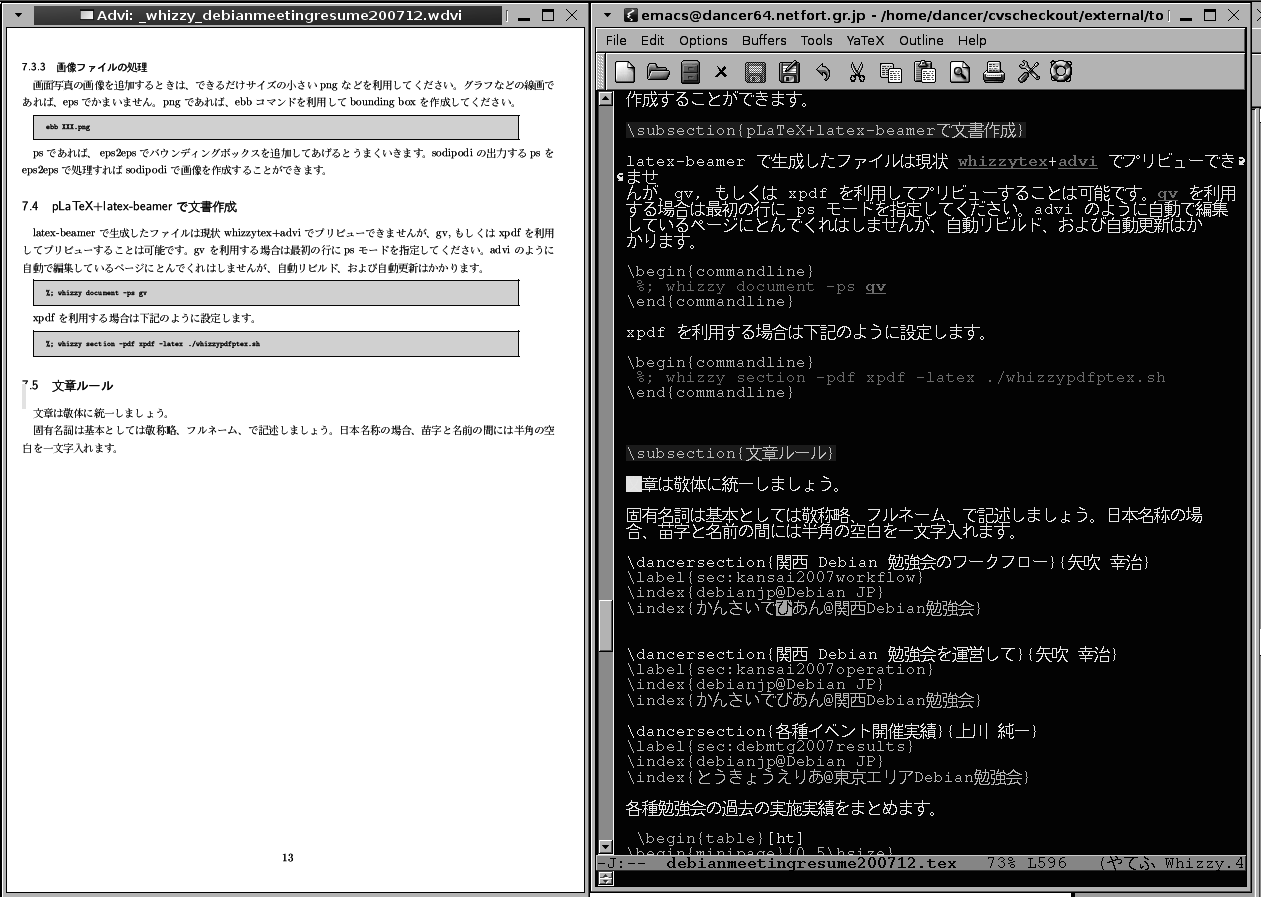
\includegraphics[width=1\hsize]{image200712/whizzytex_mono.png}

%201304
%-------------------------------------------------------------------------------
\dancersection{Debian勉強会予約システム変更履歴}{上川純一}
%-------------------------------------------------------------------------------
\index{Debianべんきょうかいよやくしすてむ@Debian勉強会予約システム}

Debian勉強会の予約システムの機能をいくつか変更したので報告します。

\subsection{アンケートのリマインダ}

\begin{wrapfigure}{r}{30zw}
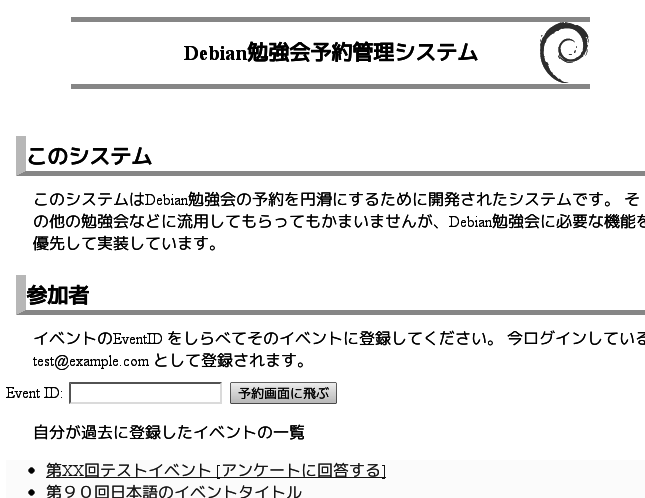
\includegraphics[width=1\hsize]{image201304/enquetereminder_mono.png}
\end{wrapfigure}

アンケートを送付していますが、現状メールで通知しているのみで、メールから
しかアンケート回答できません。
勉強会に登録している場合にアンケートを依頼してもメールがとどいていないと
かメールに気づいていないというフィードバックをもらいました。

しかしながらメール通知以外で勉強会のあとにウェブページに来てもらうという
のは難しいと思うのですが、ものは試しという事でトップページにリンクを表示
するようにして見ました。参加しているイベントでアンケートの質問が作成され
ていてアンケートの回答がまだなされていない場合にアンケートのリンクを表示
します。


\subsection{勉強会に登録した時刻}

SVGでなにができるのか試してみる勉強のついでに勉強会幹事用のページにグラ
フを出すようにして見ました。時刻を10に分割してそれぞれの時刻においての
登録の頻度の推移をみれるようにしています。このグラフを見ることでどのイベ
ントでいつごろ何人登録したのかがわかります。
試しに最近の二回を見てみたのですがけっこう違いますね。

HTML5 においてSVGの画像をうめこむのは結構簡単で、そのままSVGタグを埋め込め
ばいいだけです。inkscapeの吐くSVGをみて手書きは無理かなと思っていたので
すが基本的な記法だけであれば手書きするのも悪くはないと思える書式でした。
\index{svg}

\begin{commandline}
 <svg width="800" height="120">
	  <text x="0" y="120">2012-11-03</text>
	  <text x="400" y="120">2012-11-17</text>
	  <text x="0" y="100">0</text>
	  <text x="0" y="16">6</text>
	  <polyline points="
 0,83.3333333333
 50,66.6666666667
 100,83.3333333333
 150,100.0
 200,100.0 
 250,100.0 
 300,100.0 
 350,100.0 
 400,0.0 
 450,33.3333333333 " 
          fill="none" stroke="#333">
	  </polyline>
    </svg>
\end{commandline}

\begin{figure}[ht]
\begin{minipage}{0.5\hsize}
 \begin{center}
  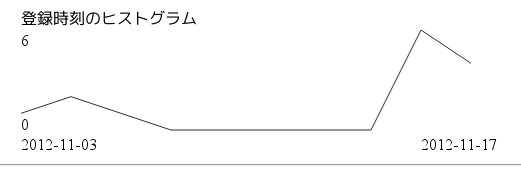
\includegraphics[width=1\hsize]{image201304/attendgraph1.png}
 \end{center} 
 \caption{2012年11月の勉強会の登録時刻}
\end{minipage}
\begin{minipage}{0.5\hsize}
\begin{center}
  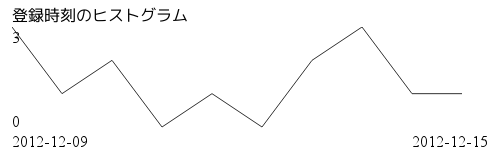
\includegraphics[width=1\hsize]{image201304/attendgraph2.png}
\end{center} 
\caption{2012年12月の勉強会の登録時刻}
\end{minipage}
\end{figure}

\subsection{コミット数}

\begin{figure}[ht]
\begin{minipage}{0.5\hsize}
気になったのでコミット数のグラフを作成してみました。四半期ごとにプロット
しています。年末に集中してコミットしているのが見て取れます。しばらくいじっ
てない気がしていましたが年に一回くらいは頑張っていじってる時期があるみた
いですね。一年を振り返るついでにいろいろ弄りたくなるのかもしれません。
\end{minipage}
\begin{minipage}{0.5\hsize}
\begin{center}
\includegraphics[width=1\hsize]{image201304/util-gae-commits.eps}
\end{center} 
\caption{各四半期毎におけるutil/gaeディレクトリのgitコミット数}
\end{minipage}
\end{figure}

%201301tokyo
\dancersection{Debian勉強会予約システムアンケート集計}{上川 純一}
%-------------------------------------------------------------------------------
\index{Debianべんきょうかいよやくしすてむ@Debian勉強会予約システム}
\index{あんけーと@アンケート}
\index{R}

\subsection{アンケート集計結果の処理}

東京エリアDebian勉強会ではアンケートをとっています。集計結果を眺めてみま
しょう。データはDebian勉強会予約システムのアンケート出力インタフェース
\url{http://debianmeeting.appspot.com/enquete/showallresults}から取得し
ます\footnote{取得したファイルを \url{image201301/enquete.csv} において
おきます。}
出力形式は各行がDebian勉強会予約システムに登録している個人で、各列がそれ
ぞれのセッションです。各コラム名は一意なキーとして扱えるようにするためイベン
ト名とセッション名を足してかつイベントのハッシュ値の一部を追加したものを
採用しています。

R で処理するためにデータを読み込み前処理を行うのには便利なスクリプトを用
意しているのでそれを利用します。

\begin{commandline}
> source('getenquete.R')
\end{commandline}

まず全体的なスコアのつき方から紹介しましょう。
\fgref{fig:enquete-score-distribution}にすべてのお題のスコアの分布を並べ
ています。時系列にならんではいますがそれぞれのテーマごとに並んでいるので
時系列とは限りません。

\fgref{fig:all-enquete-score-distribution}に平均点がどういう分布をしてい
るのかを図示しています。八割くらいは4点になり、一割づつ5点と3点があるよう
なスコア分布であることが見て取れます。特にひどいときには平均点が2点になっ
てるような気もします。ここから読み取れる全体的な傾向としては、ほとんどの場合は平均点で、特によいときに
は良い点数、特に悪い時には悪い点数をつけている人が多いということでしょう
か。

\begin{figure}[ht]
\begin{minipage}{0.5\hsize}
 \begin{center}
  \includegraphics[width=0.8\hsize,angle=270]{image201301/enquete_boxplot.eps}
 \end{center} 
 \caption{毎回のスコアの分布}\label{fig:enquete-score-distribution}
\end{minipage}
\begin{minipage}{0.5\hsize}
\begin{center}
  \includegraphics[width=0.8\hsize,angle=270]{image201301/raw_average_score_density.eps}
\end{center} 
 \caption{すべての回を通しての平均点の分布}
 \label{fig:all-enquete-score-distribution}
\end{minipage}
\end{figure}

データの癖を確認するために代表的なユーザの例を見てみます。
\fgref{fig:example-user-score-1}\fgref{fig:example-user-score-2}にどのス
コアを何度つけたのかをグラフにしています。ほとんどの場合は4をつけて、一
部に5、3をつけ、2と1はほとんどつけてないという結果になっています。こ
れに数回しか評価に参加していないユーザが4をつけるなどのバイアスが加わっ
て全体としては4がさらに強調されているような気もします。

\begin{figure}[ht]
\begin{minipage}{0.5\hsize}
 \begin{center}
  \includegraphics[width=0.8\hsize,angle=270]{image201301/score_hist_8.eps}
 \end{center} 
 \caption{あるユーザのつけたスコア分布}
 \label{fig:example-user-score-1}
\end{minipage}
\begin{minipage}{0.5\hsize}
\begin{center}
 \includegraphics[width=0.8\hsize,angle=270]{image201301/score_hist_9.eps}
\end{center} 
 \caption{また別のユーザのつけたスコア分布}
 \label{fig:example-user-score-2}
\end{minipage}
\end{figure}

気になるのでセッションの具体例をみてみましょう。2010年12月の勉強会のDebian Miniconf企画
会議はぐだぐだだったので仕方がないでしょう。一方、
2012年1月の事前課題紹介に辛口の評価が多かったのが気になります。n=4 なのでそん
なに少数派でもないようです。今から振り返ってもいまいちぱっとしない内容な
のですが運営がまずかったのでしょうか。

\begin{commandline}
> raw_average_score[!is.na(raw_average_score) & raw_average_score < 3]
                第71回東京エリアDebian勉強会.2010年12月勉強会.Debian.Miniconf.企画.2eca 
                                                                               2.333333 
              第84回東京エリアDebian勉強会.2012年1月勉強会.事前課題紹介.2012年企画.f447 
                                                                               2.500000 
第84回東京エリアDebian勉強会.2012年1月勉強会.第3回月刊Debhelper.dh_auto_..dh_build.f447 
                                                                               2.500000 
> enquete_response[!is.na(raw_average_score) & raw_average_score < 3]
                第71回東京エリアDebian勉強会.2010年12月勉強会.Debian.Miniconf.企画.2eca 
                                                                                      6 
              第84回東京エリアDebian勉強会.2012年1月勉強会.事前課題紹介.2012年企画.f447 
                                                                                      4 
第84回東京エリアDebian勉強会.2012年1月勉強会.第3回月刊Debhelper.dh_auto_..dh_build.f447 

> scaled_average_score['第84回東京エリアDebian勉強会.2012年1月勉強会.事前課題紹介.2012年企画.f447']
第84回東京エリアDebian勉強会.2012年1月勉強会.事前課題紹介.2012年企画.f447 
                                                                -1.289405 
                                                                                      4 
\end{commandline}

一方でハイスコア側を眺めてみましょう。最高のスコアは「第79回東京エリア
Debian勉強会.2011年8月勉強会.Debianパッケージのビルド方法」と「第91回東京
エリアDebian勉強会.2012年8月勉強会.月刊.Debhelper.共有ライブラリ編」です。
それぞれn=2とn=3で全員最高点を指定した結果です。アンケートに回答してくれ
た人数が少ないのが気になりますが、力作で聞いてておもしろいものでした。
「第72回東京エリアDebian勉強会.2011年1月勉強会.Kinect」$ 4.875 (sd=0.35,
n=8)$ と「第95回東京エリアDebian勉強会.2012年12月勉強会.著作権法改正」
$4.75 (sd=0.5, n=4)$ が比較的投票数も高くてスコアの高いものです。Kinectは
デモ満載でやっていることもぶっ飛んでました。著作権法改正については問題意
識を刺激する内容だったのではないでしょうか。

\begin{commandline}

>  raw_average_score[!is.na(raw_average_score) & raw_average_score > 4.5]
      第71回東京エリアDebian勉強会.2010年12月勉強会.CACertの準備に何が必要か.2eca 
                                                                         4.600000 
       第71回東京エリアDebian勉強会.2010年12月勉強会.俺のlibsaneが火をふくぜ.2eca 
                                                                         4.666667 
                         第72回東京エリアDebian勉強会.2011年1月勉強会.Kinect.f456 
                                                                         4.875000 
   第79回東京エリアDebian勉強会.2011年8月勉強会.Debianパッケージのビルド方法.5dff 
                                                                         5.000000 
            第91回東京エリアDebian勉強会.2012年8月勉強会.DebianでC..11を使う.9796 
                                                                         4.666667 
第91回東京エリアDebian勉強会.2012年8月勉強会.月刊.Debhelper.共有ライブラリ編.9796 
                                                                         5.000000 
                  第95回東京エリアDebian勉強会.2012年12月勉強会.著作権法改正.3f15 
                                                                         4.750000 
> enquete_response[!is.na(raw_average_score) & raw_average_score > 4.5]
      第71回東京エリアDebian勉強会.2010年12月勉強会.CACertの準備に何が必要か.2eca 
                                                                                5 
       第71回東京エリアDebian勉強会.2010年12月勉強会.俺のlibsaneが火をふくぜ.2eca 
                                                                                3 
                         第72回東京エリアDebian勉強会.2011年1月勉強会.Kinect.f456 
                                                                                8 
   第79回東京エリアDebian勉強会.2011年8月勉強会.Debianパッケージのビルド方法.5dff 
                                                                                2 
            第91回東京エリアDebian勉強会.2012年8月勉強会.DebianでC..11を使う.9796 
                                                                                3 
第91回東京エリアDebian勉強会.2012年8月勉強会.月刊.Debhelper.共有ライブラリ編.9796 
                                                                                3 
                  第95回東京エリアDebian勉強会.2012年12月勉強会.著作権法改正.3f15 
                                                                                4 
 
\end{commandline}


\subsection{アンケートの設計について}

今回みられた現象としては、5段階評価の4に評価が集まってしまいました。素
朴にとらえると「よい」といってもらえていることになります。しかしこれだと
分解能が低いと捉えることもできます。

これは「中心化傾向」もしくは
「寛大化傾向」とよばれる現象にあてはまると思います。

アンケート設計の世界ではそれなりにいろいろな対策方法が存在しているようで
すがまだ僕がよく理解できてません。

\clearpage % flush images.

%201212kansai
\dancersection{2012年の振り返りと2013年の企画}{佐々木洋平/Debian JP Project}

今月が 2012 年最後の関西 Debian 勉強会になります。
初回が 2007 年 3 月ということで、今年で 6 年目になりますね。
今年は定例となっている OpenSource 関連のイベントへの参加だけではなく
「大統一Debian勉強会」を開催することができたのが大きな収穫だと思っています。

\subsection{勉強会全体について}

\subsubsection{月刊Debian Policy}
今年は「月刊物をなんかやってみないか?」ということで「月刊 Debian Policy」を始めてみました。
Debian Policy Manual, version 3.9.1 の日本語訳は Debian JP Project によって公開されています
\footnote{
  \texttt{http://www.debian.or.jp/community/devel/debian-policy-ja/policy.ja.html/}
}。「月刊 Debian Policy」では、
最新の Debian Policy Manual
\footnote{
  \texttt{http://www.debian.org/doc/debian-policy/}\newline
  現時点での最新版は 3.9.4.0, 2012-09-19
} を読み進めて勉強しながら、
現在公開されている日本語訳と突き合わせつつ、
(あわよくば)これを更新したいと考えています。
「Debian Policy Manual を勉強する」という目的は毎回の勉強会で非常に上手く進んでいると思います。
今後も進めて行きたいと思いますが、如何でしょうか。

\subsubsection{翻訳ネタ}

今年後半の関西Debian勉強会では「翻訳」に関する発表が幾つか行なわれました。
「翻訳」されて母国語で文書が読めることは、
ソフトウェアの普及やコミュニティの参加への敷居を下げるという点で、非常に重要です。
Debian JP では(不幸な事に)、作業プロセスが不透明であったり、
幾つかの(非常に重要な)翻訳作業が属人化している、という問題もあります。
今年の勉強会でせっかく盛り上がりつつある「翻訳熱」を冷ますことなく、
今後はなんらかの改善が行なわれると良いかな、と思っています。

\subsubsection{その他, 定例ネタ}

毎回のセッションについてですが、
今年は「パッケージ作成」や「BTS」に関する題材として「t-code」「Konoha」に関するお話を複数回にわたって発表して頂きました。
具体的に弄りたいパッケージがあると、(発表者のモチベーションが違うのか)非常に良い勉強会になった気がします。
来年は Wheezy がリリースされることですし、
定番のネタ(Debianの入門的なお話、ライセンス、パッケージ作成、BTS)などの題材に加えて、
「Wheezy から始める Debian 環境」みたいなお話もあったら良いかな、と考えています。
昨年は案が出たけで結局実施できなかった「インストール大会」のような初心者講習もやってみたい所ですね。

\subsection{運営}

運営に関しては、今年の(特に後半は)河田さんの獅子奮迅の活躍により勉強会が開催できていました。
運営側が多忙となってしまうのはある程度しかたない(かもしれない)ですが、
今後はもう少し個人の負担を減らしつつ開催していきたいと考えています。

\subsection{イベント/NM申請}

イベント参加については、OSC Kansai@Kyoto, KOF 2012 に参加しました。
勉強会から fork した GPG キーサインパーティも毎回実施されています。今後も継続して参加する予定です。
%
また、1月には関西初の「Debian 温泉合宿」が、6月には東京エリアDebian勉強会と合同で「大統一Debian勉強会」を開催しました。
これらのイベントは今後も継続して実施する予定です。

Debian 開発者への道、として佐々木と倉敷さんの二人が NM プロセスにて DD になるための申請中です。
今後も NM プロセスに挑む参加者や Debian Maintainer となって精力的にパッケージを開発/更新する人が増えると良いですね。

\subsection{開催実績}

関西Debian勉強会の出席状況を確認してみましょう。グラフで見る
と\fgref{fig:kansaipeoplechart}になります。また、毎回の参加者の人数とその
際のトピックを \tbref{tab:count2012kansai} にまとめました。グラフ中の黒線
は参加人数、赤線は1年の移動平均です。参加人数が$0$となっているところは人
数が集計されていないor開催されなかった月です。

Debian勉強会申し込みシステムを使用するようになり、事前課題を設定すること
も多くなりました。また、アンケートシステムも稼動するようになるでしょうか
ら、今後は事前課題と事後課題のグラフを追加しようと思っています。
%
\begin{figure}[h]
  \begin{center}
    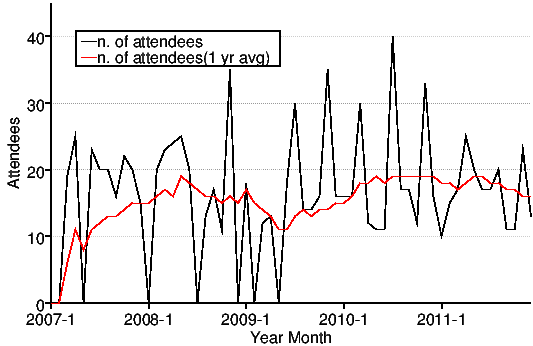
\includegraphics[width=.6\hsize]{image201212/memberanalysis/kansai.png}
  \end{center}
  \caption{関西の参加人数推移(参加人数と6ヶ月移動平均)}
  \label{fig:kansaipeoplechart}
\end{figure}

%\pagebreak

\begin{table}
  \begin{minipage}{.5\linewidth}
  \caption{関西Debian勉強会の参加人数とトピック(2007-2008年)}
  \begin{center}
    \begin{tabular}{|l|c|p{10em}|}
      \hline
                 & 参加人数 & 内容 \\
      \hline
      2007年3月  & 19       & 開催にあたり \\
      2007年4月  & 25       & goodbye、youtube、プロジェクトトラッカー\\
      2007年6月  & 23       & 社会契約、テーマ、debian/rules、bugreport\\
      2007年7月  & 20前後   & OSC-Kansai \\
      2007年8月  & 20       & Inkscape、patch、dpatch\\
      2007年9月  & 16       & ライブラリ、翻訳、debtorrent\\
      2007年10月 & 22       & 日本語入力、SPAMフィルタ\\
      2007年11月 & 20前後   & KOF \\
      2007年12月 & 15       & 忘年会、iPod touch\\
      \hline
      \hline
                 & 参加人数 & 内容 \\
      \hline
      2008年2月  & 20       & PC Cluster, GIS, \TeX \\
      2008年3月  & 23       & bug report, developer corner, GPG \\
      2008年4月  & 24       & coLinux, Debian GNU/kFreeBSD, sid \\
      2008年5月  & 25       & ipv6, emacs, ustream.tv\\
      2008年6月  & 20       & pbuilder, hotplug, ssl\\
      2008年8月  & 13       & coLinux \\
      2008年9月  & 17       & debian mentors, ubiquity, DFSG\\
      2008年10月 & 11       & cdbs,cdn.debian.or.jp \\
      2008年11月 & 35       & KOF \\
      2008年12月 & ?        & TeX資料作成ハンズオン\\
      \hline
    \end{tabular}
  \end{center}
\end{minipage}
\pagebreak
\begin{minipage}{.5\linewidth}
  \begin{center}
    \caption{関西Debian勉強会の参加人数とトピック(2009-2010)}
    \begin{tabular}{|l|c|p{10em}|}
      \hline
                 & 参加人数 & 内容 \\
      \hline
      2009年1月  & 18       & DMCK, LT \\
      2009年3月  & 12       & Git \\
      2009年4月  & 13       & Installing sid, Mancoosi, keysign \\
      2009年6月  & 18       & Debian Live, bash\\
      2009年7月  & 30?      & OSC2009Kansai \\
      2009年8月  & 14       & DDTSS, lintian \\
      2009年9月  & 14       & reportbug, debian mentors\\
      2009年10月 & 16       & gdb, packaging \\
      2009年11月 & 35       & KOF2009 \\
      2009年12月 & 16       & GPS program, OpenStreetMap \\
      \hline
      \hline
                 & 参加人数 & 内容 \\
      \hline
      2010年1月  & 16       & Xen, 2010年企画 \\
      2010年2月  & 16       & レンタルサーバでの利用, GAE \\
      2010年3月  & 30?      & OSC2010Kobe \\
      2010年4月  & 12       & デスクトップ環境, 正規表現 \\
      2010年5月  & 11       & ubuntu, squeeze \\
      2010年6月  & 11       & debhelper7, cdbs, puppet \\
      2010年7月  & 40?      & OSC2010Kyoto \\
      2010年8月  & 17       & emdebian, kFreeBSD \\
      2010年9月  & 17       & タイルWM \\
      2010年10月 & 12       & initramfs, debian live \\
      2010年11月 & 33       & KOF2010 \\
      2010年12月 & 14       & Proxmox, annual review \\
      \hline
    \end{tabular}
  \end{center}
\end{minipage}
\end{table}
\pagebreak
\begin{table}
%  \begin{minipage}{.5\linewidth}
    \caption{関西Debian勉強会の参加人数とトピック(2011)}
    \begin{center}
      %\begin{tabular}{|l|c|p{10em}|}
      \begin{tabular}{|l|c|l|}
        \hline
        開催年月  & 参加人数 & 内容 \\
        \hline
        2011年1月 &10        & BTS, Debian GNU/kFreeBSD\\
        2011年2月 &15        & pbuilder, Squeezeリリースパーティ\\
        2011年3月 &17        & ライセンス, Debianのドキュメント関連\\
        2011年4月 &25        & OSC 2011 Kansai @ Kobe, GPG キーサインパーティ \\
        2011年5月 &20        & vi, dpkg \\
        2011年6月 &17        & IPv6, vcs-buildpackage{svn, git}\\
        2011年7月 &17        & OSC 2011 Kansai @ Kyoto, GPG キーサインパーティ\\
        2011年8月 &20        & Debianパッケージ作成ハンズオン\\
        2011年9月 &11        & vcs-buildpackage{bzr, git}\\
        2011年10月&11        & Emacs, vim の拡張のDebianパッケージ, 翻訳\\
        2011年11月&23        & KOF 2011\\
        2011年12月&13        & NMプロセス, BTS\\
        \hline
      \end{tabular}
    \end{center}
%  \end{minipage}
%  \begin{minipage}{.5\linewidth}
    \caption{関西Debian勉強会の参加人数とトピック(2012)}
    \label{tab:count2012kansai}
    \begin{center}
%      \begin{tabular}{|l|c|p{10em}|}
      \begin{tabular}{|l|c|l|}
        \hline
        開催年月  & 参加人数 & 内容 \\
        \hline
        2012年1月 & 7        & Debian温泉合宿 \\
        2012年2月 &14        & autofs+pam\_chroot, t-codeその1, 月刊Debian Policy その1 \\
        2012年3月 &12        & 新年度スケジューリング, Konohaその1, t-codeその2, 月刊Debian Policy その2 \\
        2012年4月 &12        & フリーソフトウェアと著作権, Konohaその2, 月刊Debian Policy その3 \\
        2012年5月 &13        & DebianとLDAP(頓挫), ITP入門, 月刊Debian Policy その4 \\
        2012年6月 & -        & 大統一Debian勉強会 \\
        2012年7月 &10        & DebianとLDAPその1, 大統一Debian勉強会報告, 月刊Debian Policy その5 \\
        2012年8月 &28        & OSC 2012 Kansai @ Kyoto, GPG キーサインパーティ\\
        2012年8月 &16        & DebianとKerberos, News from EDOS \\
        2012年9月 & 8        & clang によるパッケージビルド, 月刊Debian Policy その6 \\
        2012年10月&14        & 翻訳環境構築, DSAの舞台裏\\
        2012年11月&34        & KOF 2012\\
        2012年12月&12        & Debian on Android, 月刊Debian Policy その7 \\
        \hline
      \end{tabular}
    \end{center}
%  \end{minipage}
\end{table}
\clearpage 

%201212tokyo
%-------------------------------------------------------------------------------
\dancersection{2012年度東京エリアDebian勉強会の振り返り}{上川 純一}
%-------------------------------------------------------------------------------

今月で8年目の東京エリアDebian勉強会が終了しました。

\subsection{基本的な数値}

出席数の推移をみましょう。最近は出席が把握できていない回が多いのですが、
だいたい参加者数12人くらいで推移しているようです(\fgref{fig:tokyoattend2012})。
事前課題の提出数(\fgref{fig:tokyoprework2012})は最近は安定していて提出率が向上しているようです。

\begin{figure}[htbp]
 \begin{minipage}{0.5\hsize}
  \begin{center}
 \includegraphics[width=0.7\hsize,angle=270]{image201212/memberanalysis/attend.eps}
  \end{center}
\caption{東京エリアDebian勉強会出席実績(12ヶ月移動平均)}\label{fig:tokyoattend2012}
  \label{fig:one}
 \end{minipage}
 \begin{minipage}{0.5\hsize}
  \begin{center}
 \includegraphics[width=0.7\hsize,angle=270]{image201212/memberanalysis/prework.eps}  \end{center}
\caption{東京エリアDebian勉強会事前課題提出実績(12ヶ月移動平均)}\label{fig:tokyoprework2012}
  \label{fig:two}
 \end{minipage}
\end{figure}

\subsection{過去のテーマ}

過去のテーマを眺めてみましょう。2012年は月刊Debhelperを中心にDebianパッケー
ジ開発の基本的な部分をおさえつつ、Debianを使って開発する開発者のための応
用的なテーマについて多くとりあげたと思います。

\begin{table}[ht]
\begin{minipage}{0.5\hsize}
 \caption{東京エリアDebian勉強会参加人数(2005-2006年)}\label{tab:count2005}
 \begin{center}
  \begin{tabular}{|l|c|p{10em}|}
 \hline
   & 参加人数 & 内容 \\
 \hline
   2005年1月 & 21 & 秘密\\
   2005年2月 & 10 & debhelper 1\\
   2005年3月 & 8 &  (早朝) debhelper 2、social contract\\
   2005年4月 & 6 & debhelper 3\\
   2005年5月 & 8 & DFSG、dpkg-cross、lintian/linda\\
   2005年6月 & 12 & alternatives、d-i\\
   2005年7月 & 12 & toolchain、dpatch\\
   2005年8月 & 7 & Debconf参加報告、ITPからアップロードまで\\
   2005年9月 & 14 & debconf\\
   2005年10月 & 9 & apt-listbugs、バグレポート、debconf翻訳、debbugs\\
   2005年11月 & 8 & DWN翻訳フロー、statoverride\\
   2005年12月 & 8 & 忘年会\\
   2006年1月 & 8 & policy、Debian勉強会でやりたいこと\\
   2006年2月 & 7 & policy、multimedia \\
   2006年3月 & 30 & OSC: debian勉強会、sid \\
   2006年4月 & 15 & policy、\LaTeX{} \\
   2006年5月 & 6 & mexico \\
   2006年6月 & 16 & debconf、cowdancer\\
   2006年7月 & 40 & OSC-Do: MacBook Debian \\
   2006年8月 & 17 & 13執念 \\
   2006年9月 & 12 & 翻訳、Debian-specific、oprofile \\
   2006年10月 & 23 & network、i18n会議、Flash、apt \\
   2006年11月 & 20 & 関西開催: bug、sid、packaging \\
   2006年12月 & 14 & 忘年会 \\
 \hline
  \end{tabular}
 \end{center}
\end{minipage}
\begin{minipage}{0.5\hsize}
 \caption{東京エリアDebian勉強会参加人数(2007-2008年)}\label{tab:count2007}
 \begin{center}
  \begin{tabular}{|l|c|p{10em}|}
 \hline
 & 参加人数 & 内容\\
 \hline
   2007年1月 & 15 & 一年を企画する \\
   2007年2月 & 13 & dbs, dpatch\\ 
   2007年3月 & 80 & OSC仮想化 \\
   2007年4月 & 19 & quilt, darcs, git\\
   2007年5月 & 23 & etch, pbuilder, superh \\   
   2007年6月 & 4 & エジンバラ開催:Debconf7 実況中継 \\
   2007年7月 & 18 & Debconf7 参加報告\\
   2007年8月 & 25 & cdn.debian.or.jp \\   
   2007年9月 & 14 & exim \\   
   2007年10月 & 30 & OSC Tokyo/Fall(CUPS) \\   
   2007年11月 & 19 & live-helper, tomoyo linux kernel patch, server\\
   2007年12月 & 11 & 忘年会\\
   2008年1月 & 23 & 一年を企画する \\
   2008年2/29,3/1 & 36 & OSC  \\
   2008年3月 & 37 & データだけのパッケージ、ライセンス \\
   2008年4月 & 17 & バイナリパッケージ \\
   2008年5月 & 20 & 複数のバイナリパッケージ \\
   2008年6月 & 10 & debhelper \\
   2008年7月 & 17 & Linux kernel patch / module パッケージ \\
   2008年8月 & 10 & Debconf IRC会議とDebian温泉 \\
   2008年9月 & 17 & po4a, 「Debian メンテナのお仕事」 \\
   2008年10月 & 11? & OSC Tokyo/Fall \\
   2008年11月 & 17 & 「その場で勉強会資料を作成しちゃえ」 Debian を使った \LaTeX{} 原稿作成合宿 \\
   2008年12月 & 12 & 忘年会 \\
 \hline
  \end{tabular}
 \end{center}
\end{minipage}
\end{table}

\begin{table}[t]
\begin{minipage}{0.5\hsize}
 \caption{東京エリアDebian勉強会参加人数(2009-2010年)}\label{tab:count2009}
 \begin{center}
  \begin{tabular}{|l|c|p{10em}|}
 \hline
 & 参加人数 & 内容\\
 \hline
   2009年1月 & 12 & 一年を企画する \\
   2009年2月 & 30 & OSC パッケージハンズオン\\ 
   2009年3月 & 23 & Common Lisp, パッケージ作成 \\
   2009年4月 & 15 & Java Policy, ocaml, 開発ワークフロー\\
   2009年5月 & 13 & MC-MPIパッケージ化、Erlang、Androidアプリ、DDTP \\   
   2009年6月 & 14 & DDTP・DDTSS、bsdstatsパッケージ、Debian kFreeBSD\\
   2009年7月 & 4 & スペインにてDebconf 9\\
   2009年8月 & 14 & スペイン Debconf 9 参加報告 \\   
   2009年9月 & 26 & GPGキーサインパーティー \\   
   2009年10月 & 30 & OSC Tokyo Fall\\
   2009年11月 & 12 & Octave, R, gnuplot, auto-builder \\
   2009年12月 & 10 & 忘年会\\
   2010年1月 & 17 &  東京大学にて新年会 \\
   2010年2月 & 11 & Debian温泉,ocaml,haskell \\
   2010年3月 & 12 & weka,fftw,dpkg v3 quilt \\
   2010年4月 & 15 & upstart,piuparts,debtags \\
   2010年5月 & 22 & 筑波大学,kernel \\
   2010年6月 & 12 & OSC-Doリハーサル  \\
   2010年7月 & 0 & キャンセル  \\
   2010年8月 & 3 & Debconf (NYC) \\
   2010年9月 & 30 & OSC Tokyo/Fall \\
   2010年10月 & 13 & 俺のDebianな一日 \\
   2010年11月 & 15 & ext4,btrfs,nilfs,ceph \\
   2010年12月 & 14 &  cacert, libsane \\
 \hline
  \end{tabular}
 \end{center}
\end{minipage}
\begin{minipage}{0.5\hsize}
 \caption{東京エリアDebian勉強会参加人数(2011-2012年)}\label{tab:count2011}
 \begin{center}
  \begin{tabular}{|l|c|p{12em}|}
 \hline
 & 人数 & 内容\\
 \hline
   2011年1月 & 12 & Kinect,アンケートシステム,CACertサイン会 \\
   2011年2月 & 13 & HDFS,Debian Game Team \\
   2011年3月 & ? & OSC Tokyo / Spring, CACert ATE Tokyo \\
   2011年4月 & 12 & IIJ, backports, initramfs, 月刊PPC64 \\
   2011年5月 & 15 & Apache2モジュール,Debian on ニフクラ,Debian/m68k,月刊PPC64 \\
   2011年6月 & 17 & ドキュメント処理系,2011再計画 \\
   2011年7月 & 3 & DebConf 11 \\
   2011年8月 & 12 & パッケージング関連, Debconf11報告 \\
   2011年9月 & 9 & 山喜旅館,Debian温泉2011 \\
   2011年10月 & 22 & 筑波大学,Haskell,LaTeX,レポート自動生成,月刊デブヘルパー開始\\
   2011年11月 & ? & OSC Tokyo/Fall \\
   2011年12月 & 9 & スクウェア・エニックス, quiltでporting, 月刊デブヘルパー,
	   振り返り \\
   2012年1月 & 8 & Debian勉強会予約システム,VPS, twitter, 
	   月刊デブヘルパー, 2012年計画 \\
   2012年2月 & 4 & KDE開発, 月刊デブヘルパー, cmake, 第0回福岡勉強会\\
   2012年3月 & ? & OSC \\
   2012年4月 & 13 & node.js, androidでDebian, 月刊デブヘルパー\\
   2012年5月 & 14 & coffeescript,python\\
   2012年6月 & ? & 大統一Debian勉強会 \\
   2012年7月 & 8? & MacBook Air 2011\\
   2012年8月 & 6? & Debconf 2012,月刊デブヘルパー,C++11 \\
   2012年9月 & 12 & OSC Tokyo Fall\\
   2012年10月 & 10 & Haskell, レゴ, xf86-input-mtrack\\
   2012年11月 & 14 & bluetooth tethering, linux perf, systemd\\
   2012年12月 & ? & 忘年会 \\

 \hline
  \end{tabular}
 \end{center}
\end{minipage}
\end{table}
\clearpage 

%201301tokyo
%-------------------------------------------------------------------------------
\dancersection{Debian勉強会2013年度計画}{上川 純一}
%-------------------------------------------------------------------------------
\index{2013ねんどけいかく@2013年度計画}

\subsection{2015年までを妄想する}

{% \tiny
\footnotesize
\begin{tabular}[t]{|p{8em}|p{12em}|p{12em}|p{8em}|p{9em}|}
%\begin{tabular}[t]{|p{8.5em}|p{12em}|p{8em}|p{6em}|p{8em}|}
\hline
2011 &2012 & 2013 & 2014 & 2015 \\
\hline
 %2011

 デスクトップパソコン終了の潮流。

 cpuコア単体では高速化しないように。

 webos終了のお知らせ。

 adobe flash復活のお知らせ(キタ), silverlight終了のお知らせ(台湾を除く)(続いてる?)

 squeezeリリース(おめでとう)

 ipv4割り当ての終了のお知らせ(キタ)

 地上波デジタル移行延長。

 btrfsまだ頑張る(fedora乙)

 java終了(sun java終了)

 open officeがoracle officeに(ナイ)

 &
 %2012

 ノートパソコンよりタブレットのほうが売れている。
 ノートパソコンではmacbookairが常識に。

 ノートパソコンでintelじゃないもの(mips/arm)が主流にはまだならず。タブレッ
 トのほうが主流。

 デスクトップ:ゲーム以外の用途では終了している。

 サーバ:個人レベルではVPS常識。企業ユースでもcloud か、vpsかを自前と比較
     検討する時代。データセンターを置く国を選べる時代。

 携帯電話:
 ガラパゴスの終焉。日本での携帯電話販売でもスマートフォンが50%を超えるように。
     ガラケー向けのネットバンクの提供が終了など、ガラケーからサービスが
     撤退し始める。
 LTE登場、普及しはじめたが、主流になっていない。
 softbankの二年契約はまだ続いている。sim freeへの道は耕されたがあたり前にならなかった。

 btrfsはまだ生き残っているがまだ使われてない?

     openstack で ceph 使う人もいる?

 mysqlからmariadbが派生。

 & 
 % 2013

コンシューマーはノートパソコンを買わなくなった。
ノートパソコンのかわりにスマートフォンを使っている。

スマートフォンが7インチくらいまで拡大、タブレットとは何だったのか。

自宅用のデスクトップパソコンのかわりに10インチくらいのタブレットを使うよ
	 うに。

サーバ:クラウドで処理するのが主流。python / ruby でコード書いていると
	 CPUが何かわからない。裏で動いているCPUは一般人は知らない。

ARMホストの仮想化技術が発達。

Oracle がメンテナンスする気がないのが明確になり、java リスクが顕著になる。

固定ゲーム機の終焉。

ゲームはARM。

 & 
 % 2014

Intel がまたARMに参入、もしくは省電力CPUを主力に切り替える。

気づいたら自作パソコン業界が終焉している。
セキュアブートが普及している。

AMD が ARM コアのCPUを出す。

Java が Oracle管理からはずれる。

スマートフォンの電池がガラケーなみに持つようになる。

電池消費が重要なアプリ選択の要素となる。
スポイトで充電できる、燃料電池が流行る。

ARメガネのプロトタイプが出てくる。

 & 
 % 2015

自作スマホの時代。
OpenHardwareがモバイルに移行する。
技適のパーツ認定基準というのができるようにがんばる。

自宅で回路が印刷できる機器が普及してCPUとかが印刷できるようになるといい
		 な。

タブレットが丸められるようになって巻物になっている。

AMD が x86 撤退。

ハードディスクを見たことがない人がいる。

データセンターを自前でもっているのは発電所を持っているところだけになる。

クラウドの法制度、免責事項、個人情報保護関連の問題が提起され、解決にむけ
		 てすすむ。
一種データセンタークラウド業者の要求規格が制定される。
ユーザ数何人以上は二種免許が必要とか。

データセンターヘイブンとよばれる国が存在する。

\\

\hline
\end{tabular}

}

2015年にどうなっているのかを妄想したところで、
2013年度の計画を立てましょう。

%
%\subsection{2013年の計画}
%
%2015年にどうなっているのかを妄想したところで、
%2013年度の計画を立てましょう。
%
%企画案:
%{\LARGE
%\begin{enumerate}
% \item 2013年の計画立案
% \item  \underline{(\hspace{10cm})}
% \item  \underline{(\hspace{10cm})}
% \item  \underline{(\hspace{10cm})}
% \item  \underline{(\hspace{10cm})}
% \item  \underline{(\hspace{10cm})}
% \item  \underline{(\hspace{10cm})}
% \item  \underline{(\hspace{10cm})}
% \item  \underline{(\hspace{10cm})}
% \item  \underline{(\hspace{10cm})}
% \item  \underline{(\hspace{10cm})}
% \item 一年間の反省
%\end{enumerate}
%}


\clearpage


%201303kansai
%原著者による GPLv2 or Later での公開に同意いただけなかったため資料は別途用意します。


%201305tokyo
%アンカンファレンス & Wheezy リリースパーティ

%-------------------------------------------------------------------------------
\dancersection{Debian Trivia Quiz}{上川 純一、岩松 信洋}
%-------------------------------------------------------------------------------

ところで、みなさん Debian 関連の話題においついていますか?Debian関連の話
題はメーリングリストをよんでいると追跡できます。ただよんでいるだけではは
りあいがないので、理解度のテストをします。特に一人だけでは意味がわからな
いところもあるかも知れません。みんなで一緒に読んでみましょう。

今回の出題範囲は\url{debian-devel-announce@lists.debian.org} や \url{debian-devel@lists.debian.org}に投稿された
内容とDebian Project Newsからです。

\begin{multicols}{2}
%; whizzy-master ../debianmeetingresume201211.tex
% $B0J>e$N@_Dj$r$7$F$$$k$?$a!"$3$N%U%!%$%k$G(B M-x whizzytex $B$9$k$H!"(Bwhizzytex$B$,MxMQ$G$-$^$9!#(B
%

\santaku
{wiki.debian.org$B$G;H$o$l$F$$$?(Bwiki$B%7%9%F%`$N%=%U%H%&%'%"$NL>A0$O!)(B}
{pukiwiki}
{mine}
{moin}
{C}
{$B@?$K0d48$J$,$i!"(Bwiki.debian.org$B$,$3$NA0%/%i%C%/$5$l$?$h$&$G$9!#(B
$BB>$GF1$8EPO?%a!<%k%"%I%l%9$H%Q%9%o!<%I$NAH$r;H$C$F$$$k?M$O!"(B
$B$9$0$K%Q%9%o!<%I$rJQ$($?J}$,$h$$$G$7$g$&!#(B}

\santaku
{$B5nG/$NG/Kv$N(Bpopcon$BD4::$G(BNo.1$B$K51$$$?%W%i%C%H%U%)!<%`$O!)(B}
{$BEvA3(Barmel$B$@$m!)(B}
{i386}
{amd64}
{C}
{\url{http://popcon.debian.org/}$B$N%H%C%W%Z!<%8$K7k2L$N%0%i%U$,$"$j$^$9!#(B
 $B:#$^$G(BNo.1$B$r7h$a$F$$$?(Bi386$B$rG/Kv$G(Bamd64$B$,H4$-5n$C$?$h$&$G$9!#(B}

\santaku
{1$B7nF,$N(BDPN$B$GJs9p$N$"$C$?!"(Bwheezy$B$K;D$C$F$$$k(BRC$B%P%0$N?t$O(B1$B7n(B5$BF|;~E@$G$"$H2?8D!)(B}
{$B$"$H(B321$B8D(B}
{$B$"$H(B171$B8D(B}
{$B$"$H(B17$B8D(B}
{B}
{$B4JC1$KD>$;$k(B/$BB><#$l$P>!<j$K<#$j$=$&$b$N$r4^$s$G(B171$B8D!#<j$,$+$+$j$=$&$J$N$O(B
$B$@$$$?$$(B116$B8D$@$=$&$G$9!#(B}

\santaku
{$B:#G/(Bamazon$B$+$i(BDebian Project$B$X$$$/$i$+$N(BAWS$B$NMxMQ7t$r%9%]%s%5!<$7$F$b$i$C$?$=$&$J$N$G$9$,!"6b3[$K$9$k$H$*$$$/$i!)(B}
{8000USD}
{800USD}
{80000USD}
{A}
{$BF|K\1_$K$9$k$HLs(B72$BK|1_J,$NMxMQ7t!#(BQA$B$K$O==J,$H$N$3$H$G$7$?!#(B}











%; whizzy-master ../debianmeetingresume201211.tex
% $B0J>e$N@_Dj$r$7$F$$$k$?$a!"$3$N%U%!%$%k$G(B M-x whizzytex $B$9$k$H!"(Bwhizzytex$B$,MxMQ$G$-$^$9!#(B
%

\santaku
{DebConf13 $B$N3+:ECO$H3+:EF|$O!)(B}
{$BF|K\!"El5~ET(B 6$B7n(B20$BF|(B}
{$B%K%+%i%0%"(B $B%^%J%0%"(B 7$B7n(B8-14$BF|(B}
{$B%9%$%9!"%t%)!<%^%k%-%e(B 8$B7n(B11-18$BF|(B}
{3}
{$B%K%+%i%0%"$O(BDebConf12$B$N3+:ECO$G$9!#(B
DebConf13$B$O%9%$%9$N%-%c%s%WCO$G3+:E$G$9!#(B
6/20$B$O3'$5$sM=Dj$r6u$1$F$*$-$^$7$g$&!#(B}

\santaku
{$B@$3&$N(BWeb$B%5!<%P$G:G$b?M5$$N$"$k(BLinux $B%G%#%9%H%j%S%e!<%7%g%s(B(W3Techs$BD4$Y(B)$B$O!)(B}
{CentOS}
{Debian}
{Ubuntu}
{B}
{\url{http://w3techs.com/technologies/history_details/os-linux}$B$K7k2L$N%0%i%U$,$"$j$^$9!#(B
$B8=:_(B Linux $B$r;HMQ$7$F$$$k(B web $B%5!<%P$N(B 32.9\% $B$,(B Debian $B$rMxMQ$7$F$*$j!"$=$N3d9g$O8=:_$bA}2C$rB3$1$F$$$k$=$&$G$9!#(B}

\santaku
{Debian $B%+!<%M%k%A!<%`$N%a%s%P!<$G$"$j!"(Bkernel.org $B$N(B 3.2.y $B0BDjHG7ONs$N%a%s%F%J$G$b$"$k(B Ben Hutchings $B$5$s$,<!4|(B Debian $B0BDjHG$H0l=o$K=P2Y$5$l$k(B Linux $B%+!<%M%k$K(B (3.2 $B7ONs$N(B mainline $B$K$OL5$$(B) $BDI2C5!G=$,Ek:\$5$l$kM=Dj$G$"$k$H=R$Y$F$$$^$9!#(B
$BB?$/$NDI2CE@$NCf$K4^$^$l$J$$$b$N$O2?!)(B}
{PREEMPT\_RT}
{Hyper-V guest drivers$B$N6/2=(B}
{ARM64/AArch64$B%"!<%-%F%/%A%c%5%]!<%H(B}
{C}
{Hyper-V guest drivers$B$O(Bmainline kernel$B$G(B3.2$B$K$b4^$^$l$F$$$^$9$,!"$h$j2~A1$5$l$?(B3.4$B$+$i$N=$@5$,F3F~$5$l$^$9!#(B
PREEMPT\_RT$B$O%O!<%I%j%"%k%?%$%`$r<B8=$9$k$?$a$N(BPatch$B!"(B
linux-image-rt-amd64 , linux-image-rt-686-pae $B$N(Bmetapackage$B$G;HMQ$G$-$^$9!#(B
$B?7$7$$(BARM 64$B%S%C%H%"!<%-%F%/%A%c%5%]!<%H$O(Bmainline kernel 3.7$B$+$i(B}

\santaku
{Wookey$B$5$s$,%"%J%&%s%9$7$?(Balpha$BHG$N(BDebian port arm64 image$B$O!)(B}
{Debian/Ubuntu port image}
{Debian/KFreeBSD port image}
{Debian/GnuHurd port image}
{A}
{self-bootstrapp(non x86)$BBP1~$H$N$3$H$G$9!#(B\url{http://wiki.debian.org/Arm64Port}$B$G%9%F!<%?%9$,3NG'$G$-$^$9!#(B}

\santaku
{700,000$BHVL\$N%P%0$,Js9p$5$l$?F|$rEv$F$k(B700000thBugContest$B$N7k2L$,=P$^$7$?!#$=$NM=A[F|$HJs9pF|$O!)(B}
{2012/12/12$B$rM=A[$7$?(BDavidPrevot}
{$BM=A[F|(B:2013/02/04$B!"Js9pF|(B:2013/02/14}
{$BM=A[F|(B:2013/02/07$B!"Js9pF|(B:2013/02/14}
{$BM=A[F|(B:2013/02/14$B!"Js9pF|(B:2013/02/07}
{C}
{$B:G$b6a$$(B2013/02/14$B$rM=A[$7$?(BChristian Perrier$B$5$s$,Ev$F$^$7$?!#7k2L$O(B\url{http://wiki.debian.org/700000thBugContest}$B$G8x3+$5$l$F$$$^$9!#(B
$B$^$?!"(B800,000/1,000,000$BHVL\$N%P%0$,Js9p$5$l$kF|$rEv$F$k%3%s%F%9%H(B\url{http://wiki.debian.org/800000thBugContest}$B$b3+:E$5$l$F$$$^$9!#(B}

\santaku
{master.debian.org$B$,?7$7$$5!3#$K0\9T$5$l$^$7$?!#$3$l$O2?$N%5!<%P$G$7$g$&$+(B $B!)(B}
{@debian.org$B$N%a!<%k%5!<%P(B}
{$B%Q%C%1!<%8$N%^%9%?!<%5!<%P(B}
{$B%Q%C%1!<%8$N%9%]%s%5!<(B(mentor)$B$rC5$9%5!<%P(B}
{A}
{$B8E$$%5!<%P$O%G%#%9%/>c32Ey$,$"$C$?$N$G!"<wL?$HH=CG$5$l!"%G!<%?$,B;<:$9$kA0$K?7$7$$%5!<%P$K0\9T$5$l$^$7$?!#(Bftp-master.debian.org$B$O(BDebian$B$N(B official package $B%j%]%8%H%j$G$9!#%Q%C%1!<%8$N%9%]%s%5!<(B(mentor)$B$rC5$9$N$O(Bmentors.debian.net$B!#(B }

\santaku
{pbuilder$B$K(Bclang support$B$,DI2C$5$l$^$7$?!#C/$,=q$$$?%Q%C%A$G$7$g$&$+!)(B}
{Sylvestre Ledru}
{Junichi Uekawa}
{Hideki Yamane}
{C}
{Debian$B$N(BClang$B%5%]!<%H$OCe!9$H?J$s$G$$$^$9!#(B}

\santaku
{DPN - 2013$BG/(B3$B7n(B4$BF|9f$K<h$j>e$2$i$l$?F|K\$N%$%Y%s%H$O(B}
{Open Source Conference 2013 Tokyo/Spring}
{Open Source Conference 2013 Hamamatu}
{Open Source Conference 2013 Tokushima}
{A}
{\url{http://henrich-on-debian.blogspot.jp/2013/02/open-source-conference-2013-tokyospring.html} $B>\:Y$O8e$[$I!#(B}


%; whizzy-master ../debianmeetingresume201304.tex
% 以上の設定をしているため、このファイルで M-x whizzytex すると、whizzytexが利用できます。
%

\santaku
{DSAのサーバを新しくホスティングしてくれるのはどれか}
{bytemark}
{grnet}
{manda}
{A}
{Debianプロジェクトのサーバ管理を担うチームがDSA、
その管理するDebianサーバのホスティングは、grnet, manda, ubcece が既存のホスティングプロバイダーで、bytemarkが今回
加わったそうです。}

\santaku
{wheezy の backports の apt-lineで適切なものはどれか}
{deb sstp://backports.debian.org/debian/ wheezy-backports backports}
{deb http://backports.debian.org/debian/ wheezy-backports main}
{deb http://ftp.debian.org/debian/ wheezy-backports main}
{C}
{backports がメインのアーカイブと統合されたようで、wheezy-backportsから
利用できるようになったようです。}

\santaku
{tech ctte 699808の結果アップロードされたのは}
{syslinux 4}
{syslinux 5}
{grub}
{A}
{新しいバージョンのsyslinuxでdebian-installerが動かないという問題があっ
てそれをダウングレードで解決したようです。}

\santaku
{あたらしくDPLになったのはだれか}
{Stephano Zacchiroli}
{Lucas Nussbaum}
{Gergely Nagy}
{B}
{Lucas が選挙の結果DPLになりました}

% \santaku
% {}
% {}
% {}
% {}
% {}
% {}


% \santaku
% {}
% {}
% {}
% {}
% {}
% {}

\end{multicols}

% 索引
\printindex

% 問題と回答が同じみひらきにならないようにする
\cleartoevenpage
%-------------------------------------------------------------------------------
\dancersection{Debian Trivia Quiz 問題回答}{上川 純一、岩松 信洋}
%-------------------------------------------------------------------------------
\\
{\small
 Debian Trivia Quiz の問題回答です。 あなたは何問わかりましたか? \\
 %回答はdebianmeetingresume2013-fuyu.jqzというファイルに生成されるので、
 %それを手動でコピペして使う。
 % ここからコピペ
 % FIXME 問題が全部はいったらコピペすること
 %(progn (next-line 1)(insert-file "debianmeetingresume2013-fuyu.jqz") )
1. C 誠に遺憾ながら、wiki.debian.orgがこの前クラックされたようです。他で同じ登録メールアドレスとパスワードの組を使っている人は、すぐにパスワードを変えた方がよいでしょう。\\
2. C \url {http://popcon.debian.org/}今までNo.1を決めていたi386を年末でamd64が抜き去ったようです。\\
3. B 簡単に直せる/他治れば勝手に治りそうものを含んで171個。手がかかりそうなのはだいたい116個。\\
4. A 日本円にすると約72万円分の利用券。QAには十分とのことでした。\\
5. C ニカラグアはDebConf12の開催地。DebConf13はスイスのキャンプ地で開催。6/29は大統一Debian勉強会。\\
6. B \url {http://w3techs.com/technologies/history_details/os-linux}に結果のグラフがあります。現在 Linux を使用している web サーバの 32.9\% が Debian を利用しており、その割合は現在も増加を続けているそうです。\\
7. B 指名期間:2013 年 3 月 3 日(日)UTC 〜 3 月 9 日(土) UTC 選挙運動期間:2013 年 3 月 10 日(日) UTC 〜 3 月 30 日(土) UTC 投票期間:2013 年 3 月 31 日(日)UTC 〜 4 月 13 日(土)UTC \url {http://www.debian.org/vote/2013/vote_001}\\
8. C Ben Hutchings さんはDebian カーネルチームのメンバーであり、kernel.org の 3.2.y 安定版系列のメンテナ。PREEMPT\_RTはI/Oの遅延と揺らぎを低減するaudio/videoアプリケーション利用等向、linux-image-rt-amd64 , linux-image-rt-686-paeで使用可能。Hyper-V guest driversは3.2にも含まれていますが、より改善された3.4からの修正を導入。TCP Fast Open(TFO)はTCPの3way-handshakeを改善し、2回目以降の通信開始時にSYNとdataを含んだパケットを送ることで高速化する技術、3.6時点ではクライアント側のみ実装、サーバ側は3.7から。\\
9. A x86環境を使用しないself-bootstrap imageです。\url {http://wiki.debian.org/Arm64Port}でステータスが確認できます。mainline kernelのARM64/AArch64(ARMv8アーキテクチャ:Cortex A57,Cortex A53予定のCPU向け)対応は 3.7から。\\
10. C 最も近い2013/02/14を予想したChristian Perrierさんが当てました。結果は\url {http://wiki.debian.org/700000thBugContest}で公開されています。また、800,000/1,000,000番目のバグが報告される日を当てるコンテスト\url {http://wiki.debian.org/800000thBugContest}も開催されています。\\
11. A 古いサーバはディスク障害等で、寿命と判断され、新しいサーバに移行されました。ftp-master.debian.orgはDebianの official package リポジトリです。パッケージのスポンサー(mentor)を探すのはmentors.debian.net。 \\
12. C Sylvestre Ledru さんはClangのメンテナーの一人です。彼はClang 3.2 を使用してアーカイブをリビルドした結果について報告しました(12.1\% が失敗、つまり18264packages中、2204が失敗)。失敗したパッケージの情報\url {http://clang.debian.net/pts.php}。DebianのClangサポートは着々と進んでいます。\\
13. A \url {http://henrich-on-debian.blogspot.jp/2013/02/open-source-conference-2013-tokyospring.html}\\
14. A Debianプロジェクトのサーバ管理を担うチームがDSA、その管理するDebianサーバのホスティングは、grnet, manda, ubcece が既存のホスティングプロバイダーで、bytemarkが今回加わったそうです。\\
15. C backports がメインのアーカイブと統合され、wheezy-backportsから利用できるようになったようです。\\
16. A 新しいバージョンのsyslinuxでdebian-installerが動かないという問題が有りダウングレードで解決したようです。\\
17. B Lucas が選挙の結果DPLになりました\\
}

\pagestyle{empty}
\cleartoevenpage

\newpage
{
\large
\begin{itembox}{\bf 『あんどきゅめんてっど でびあん』について}
本書は、東京および関西周辺で毎月行なわれている『東京エリア Debian 勉強会』(第第95回から第99回)および
『関西 Debian 勉強会』(第67回から第72回)で
使用された資料・小ネタ・必殺技などを一冊にまとめたものです。
第70回関西Debian勉強会資料は別ライセンスため無し、
第97回東京エリアDebian勉強会資料はオープンソースカンファレンス2013 Tokyo/Springのため無し、
第100回東京エリアDebian勉強会資料はアンカンファレンス & Wheezy リリースパーティのため無し、
% FIXME: 回数を修正すること。
内容は無保証、つっこみなどがあれば勉強会にて。
\end{itembox}
}

\vspace*{13cm}
{\color{dancerlightblue}\rule{\hsize}{1mm}}
\vspace{2mm}

\includegraphics[width=2cm]{image200502/openlogo-nd.eps}
\noindent \Large \bf あんどきゅめんてっど でびあん 2013年夏号\\
\noindent \normalfont 2013年8月12日 \hspace{5mm}  初版第1刷発行\\
\noindent \normalfont 東京エリア Debian 勉強会/関西エリア Debian 勉強会 (編集・印刷・発行)\\
{\color{dancerdarkblue}\rule{\hsize}{1mm}}

\end{document}
